%# -*- coding: utf-8-unix -*-
%%==================================================
%% thesis.tex
%%==================================================

% 双面打印
\documentclass[bachelor, openright, twoside]{sjtuthesis}
% \documentclass[bachelor, openany, oneside, submit]{sjtuthesis}
% \documentclass[master, review]{sjtuthesis}
% \documentclass[%
%   bachelor|master|doctor,	% 必选项
%   fontset=fandol|windows|mac|ubuntu|adobe|founder, % 字体选项
%   oneside|twoside,		% 单面打印,双面打印(奇偶页交换页边距,默认)
%   openany|openright, 		% 可以在奇数或者偶数页开新章|只在奇数页开新章(默认)
%   english,			% 启用英文模版
%   review,	 		% 盲审论文,隐去作者姓名、学号、导师姓名、致谢、发表论文和参与的项目
%   submit			% 定稿提交的论文,插入签名扫描版的原创性声明、授权声明
% ]

% 逐个导入参考文献数据库
\addbibresource{bib/thesis.bib}
% \addbibresource{bib/chap2.bib}

\begin{document}

%% 无编号内容:中英文论文封面、授权页
%# -*- coding: utf-8-unix -*-
\title{基于非连续动态对冲的场外期权定价研究}
\author{李星奇}
\studentnumber{515120910121}
\major{金融学}
\advisor{万相伟}
\defenddate{2014年12月17日}
\institute{安泰经济与管理学院}

\englishtitle{A Sample Document for \LaTeX-basedd SJTU Thesis Template}
\englishauthor{\textsc{Mo Mo}}
\englishadvisor{Prof. \textsc{Mou Mou}}
% \englishcoadvisor{Prof. \textsc{Uom Uom}}
\englishschool{Shanghai Jiao Tong University}
\englishinstitute{\textsc{Depart of XXX, School of XXX} \\
  \textsc{Shanghai Jiao Tong University} \\
  \textsc{Shanghai, P.R.China}}
\englishmajor{A Very Important Major}
\englishdate{Dec. 17th, 2014}

\maketitle

% \makeatletter
% \ifsjtu@submit\relax
% 	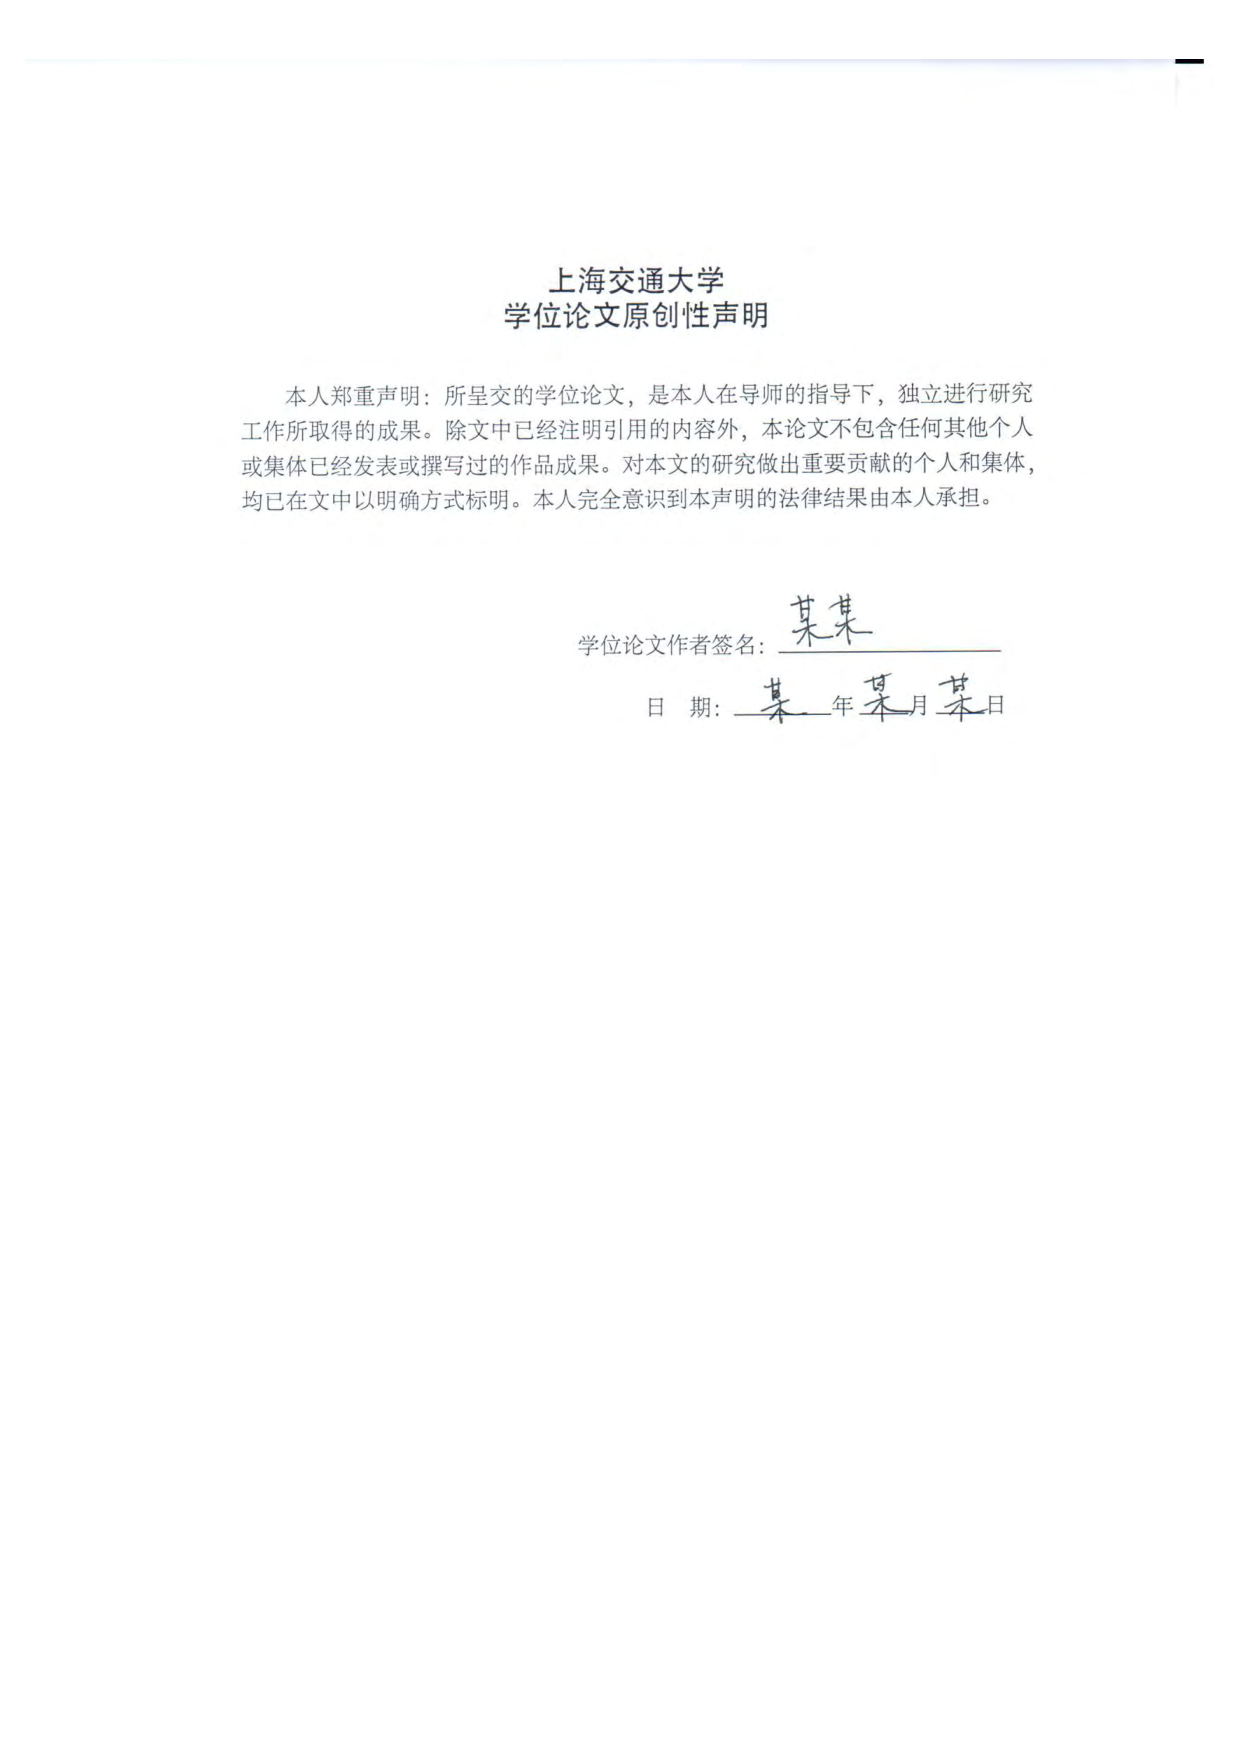
\includepdf{pdf/original.pdf}
% 	\cleardoublepage
% 	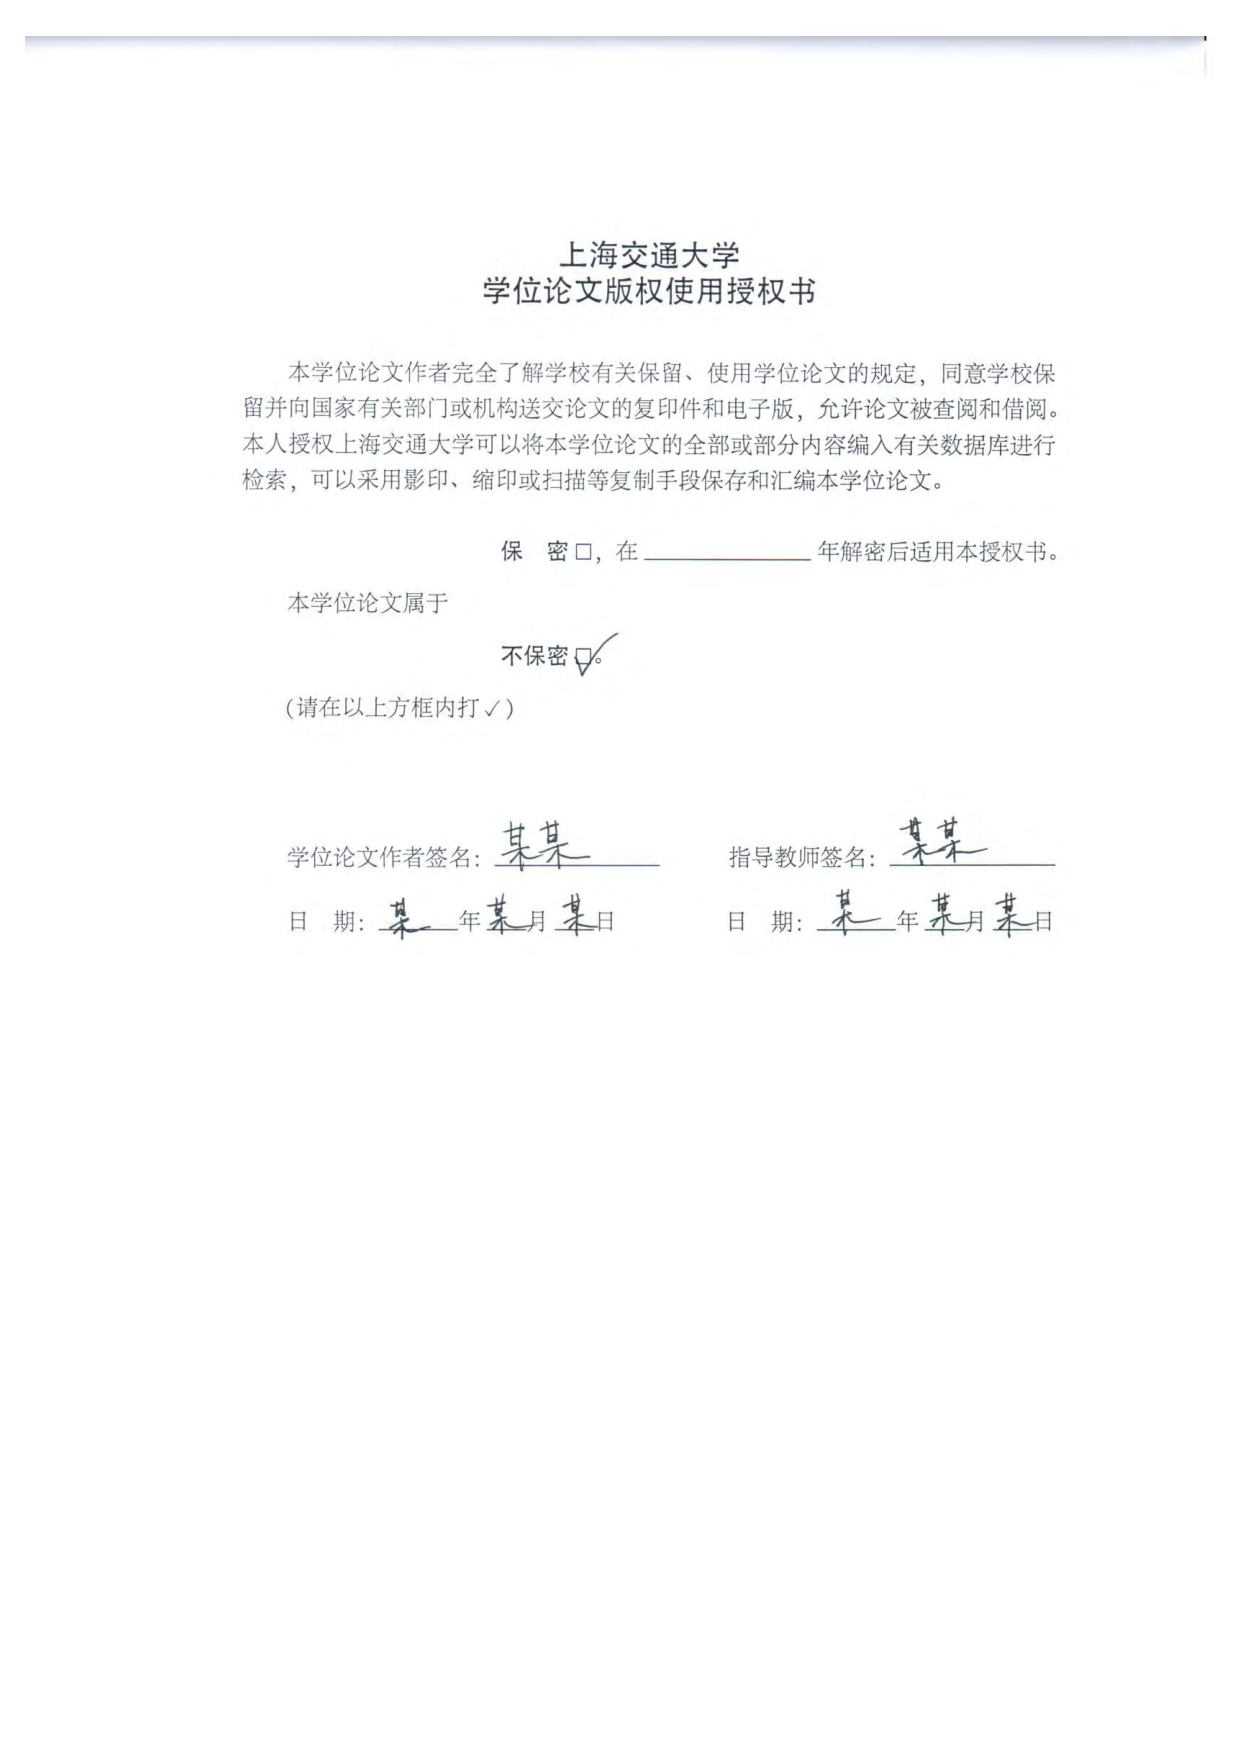
\includepdf{pdf/authorization.pdf}
% 	\cleardoublepage
% \else
% \ifsjtu@review\relax
% % exclude the original claim and authorization
% \else
% 	\makeDeclareOriginal
% 	\makeDeclareAuthorization
% \fi
% \fi
% \makeatother


\frontmatter 	% 使用罗马数字对前言编号

%% 摘要
\pagestyle{main}
%# -*- coding: utf-8-unix -*-
%%==================================================
%% abstract.tex for SJTU Master Thesis
%%==================================================

\begin{abstract}

pass

\keywords{ pass}
\end{abstract}

\begin{englishabstract}

pass

\englishkeywords{ pass}
\end{englishabstract}


%% 目录、插图目录、表格目录
\tableofcontents
% \listoffigures
% \addcontentsline{toc}{chapter}{\listfigurename} %将插图目录加入全文目录
% \listoftables
% \addcontentsline{toc}{chapter}{\listtablename}  %将表格目录加入全文目录
% \listofalgorithms
% \addcontentsline{toc}{chapter}{\listalgorithmname} %将算法目录加入全文目录

% %# -*- coding: utf-8-unix -*-
\begin{nomenclaturename}
\label{chap:symb}

\begin{longtable}{rl}
$\epsilon$     & 介电常数 \\
 $\mu$ 		& 磁导率 \\
 $\epsilon$     & 介电常数 \\
 $\mu$ 		& 磁导率 \\
 $\epsilon$     & 介电常数 \\
 $\mu$ 		& 磁导率 \\
 $\epsilon$ 	& 介电常数 \\
 $\mu$ 		& 磁导率 \\
 $\epsilon$     & 介电常数 \\
 $\mu$ 		& 磁导率 \\
 $\epsilon$     & 介电常数 \\
 $\mu$ 		& 磁导率 \\
 $\epsilon$     & 介电常数 \\
 $\mu$ 		& 磁导率 \\
 $\epsilon$ 	& 介电常数 \\
 $\mu$ 		& 磁导率 \\
 $\epsilon$     & 介电常数 \\
 $\mu$ 		& 磁导率 \\
 $\epsilon$     & 介电常数 \\
 $\mu$ 		& 磁导率 \\
 $\epsilon$     & 介电常数 \\
 $\mu$ 		& 磁导率 \\
 $\epsilon$ 	& 介电常数 \\
 $\mu$ 		& 磁导率 \\
 $\epsilon$     & 介电常数 \\
 $\mu$ 		& 磁导率 \\
 $\epsilon$     & 介电常数 \\
 $\mu$ 		& 磁导率 \\
 $\epsilon$     & 介电常数 \\
 $\mu$ 		& 磁导率 \\
 $\epsilon$ 	& 介电常数 \\
 $\mu$ 		& 磁导率 \\
 $\epsilon$     & 介电常数 \\
 $\mu$ 		& 磁导率 \\
 $\epsilon$     & 介电常数 \\
 $\mu$ 		& 磁导率 \\
 $\epsilon$     & 介电常数 \\
 $\mu$ 		& 磁导率 \\
 $\epsilon$ 	& 介电常数 \\
 $\mu$ 		& 磁导率 \\
 $\epsilon$     & 介电常数 \\
 $\mu$ 		& 磁导率 \\
 $\epsilon$     & 介电常数 \\
 $\mu$ 		& 磁导率 \\
 $\epsilon$     & 介电常数 \\
 $\mu$ 		& 磁导率 \\
 $\epsilon$ 	& 介电常数 \\
 $\mu$ 		& 磁导率 \\
 $\epsilon$     & 介电常数 \\
 $\mu$ 		& 磁导率 \\
 $\epsilon$     & 介电常数 \\
 $\mu$ 		& 磁导率 \\
 $\epsilon$     & 介电常数 \\
 $\mu$ 		& 磁导率 \\
\end{longtable}

\end{nomenclaturename}
 % 主要符号、缩略词对照表

\mainmatter	% 使用阿拉伯数字对正文编号

%% 正文内容
\pagestyle{main}
%# -*- coding: utf-8-unix -*-
%%==================================================
%% chapter01.tex for SJTU Master Thesis
%%==================================================

%\bibliographystyle{sjtu2}%[此处用于每章都生产参考文献]
\chapter{绪论}
\label{chap:intro}

\section{研究背景}

期货和期权等衍生品是金融市场和商品市场上风险管理的重要工具。
对于资产管理机构,他们可以使用金融衍生品来管理自身的beta暴露,控制系统性风险;对于实体企业,他们也可以通过买卖商品衍生品,降低由于原材料或产成品价格波动过大而带来的经营风险。
期货作为一种线性资产,其价格变动与标的价格变动呈线性关系。
实际操作中,企业可以根据未来风险的方向,按照一个套期保值比例,在期货市场上买入或卖出期货合约。原理简单、操作方便是期货的优势。
然而,使用期货进行风险管理也存在一些问题。首先,期货为保证金交易,其杠杆比率较低,因此对资金占用较高,会给企业带来较高的机会成本。更重要的是,期货的线性特性使对冲者在规避了可能的损失的同时,也放弃了未来潜在的收益。

与期货相比,期权有着独有的优势,可以有效地帮助企业解决使用期货进行风险管理时的问题。若以买入期权的方式进行对冲,则对冲者只需在期初支付一定量的期权费,在对冲期间无需关注保证金账户。并且以期权费衡量的杠杆比率也较高,用较少的资金就可以实现和期货相同的对冲头寸数量。
同时,这一对冲方式风险有限(损失全部的期权费),在价格有利变动时也可以保留获取收益的能力。因此,相比之下,期权是一种更好的对冲工具。

根据交易方式的不同,衍生品又可以分为场内衍生品(Exchange-Traded Derivatives)和场外衍生品(Over-The-Counter Derivatives)。场内衍生品又称交易所衍生品,这一类衍生品由交易双方通过交易所以竞价的方式完成交易;场外衍生品又称柜台交易衍生品,这一类衍生品由交易双方直接或通过共同对手方(Central Conterparty)进行交易和结算。与场内市场相比,场外市场通常规模更大。张玉红(2006)指出,从上世纪90年代开始,美国的场外衍生品市场的增长速度就已明显高于场内市场。同时,由于场外衍生品市场可以为企业提供特殊定制的风险管理产品,而场内市场提供的是标准化的合约。因此,场外市场和场内市场在功能上并不完全同质化。斯文(2012)通过对美国的场外衍生品市场数据进行实证分析发现,场外衍生品市场和场内市场更多地呈现出替代关系。近年来,我国场外衍生品市场发展迅猛。根据中国证券业协会的数据,截至2018年7月31日,我国场外衍生品的初始名义本金累计3.27万亿元,存量2973.54亿元。

期权这一衍生品相比于期货,涉及到更多维度的变量,企业对其的定制化需求也就更高。
因此,相比场内期权市场,我国的场外期权市场更为活跃。
目前我国场内市场中,商品期权有白糖、棉花、豆粕、玉米、铜和天然橡胶六种,金融期权有上证50ETF期权一种;而场外市场中,期权基本覆盖了大部分交易所中交易的标的。我国场外期权的交易商为证券公司和期货公司。对于这些交易商来说,他们是期权流动性的提供者,一般处于净卖出期权的位置。
他们面临着两个很实际的问题:一是如何通过场内市场复制期权,对冲自身暴露的期权头寸;二是如何根据对冲的成本对卖出的期权进行定价,以在覆盖自身对冲成本的前提下提供一个更有竞争力的价格。

我国期权市场仍处于发展阶段,与成熟市场还有较大差距。场内市场期权品种较少,无法和品种丰富的场外市场匹配,这也给上文提到的两个问题的解决增加了难度。由于缺少场内非线性的工具,交易商只能够通过使用期货或现货等线性资产来进行Delta上的动态对冲。因此,基于目前我国期权市场的现状,本文将试图对以下问题做出解答:1)如何采取恰当的Delta动态对冲策略以及确定动态对冲中的相关参数,以获得最好的对冲效果;2)在实际操作中,交易成本将在多大程度上影响最终的对冲成本。

\section{研究意义}

本文以虚拟案例的形式,使用了模拟研究和实证分析两种方法,同时基于固定时点的动态对冲和固定Delta区间的动态对冲,对场外期权的定价和对冲进行了研究。

在模拟研究中,本文使用了几何布朗运动资产价格路径模型。并且根据期权价格的特点,以波动率溢价的形式来标准化交易成本对动态对冲结果的影响。在衡量不同参数下的对冲结果时,模仿风险厌恶函数提出了一种新的评判标准,用于实际应用中动态对冲参数和具体方法的选择。

在实证分析的研究中,本文使用动力煤指数的数据,进行了滚动的动态对冲分析,以为该期权未来的定价和对冲提供一定的参考,这一框架同样适用于基于其他标的的场外和场内期权的定价。同时,将实证分析的结果和模拟研究的结果比较,有助于定性地帮助场外期权交易商理解实际应用和理论分析的差异,以更好地将动态对冲方法应用到实际生产中。

\section{研究内容}

本文分析和论述结构如下:

第一章为绪论,简要介绍了本文的研究背景、研究意义和研究内容,提出了本文研究的整体框架。

第二章为文献综述,主要介绍了目前有关方向上的研究历史及现状,包括期权定价理论和动态对冲分析的国内外相关研究。

第三章为研究方法,主要介绍了期权定价和动态对冲的基本理论及实现方法,同时将对本文所用的模拟方法以及模拟中各个参数的选取和处理进行详细介绍。

第四章为模拟与实证分析,首先给出了一个虚拟的场外期权交易案例,之后使用蒙特卡洛模拟的方法以及固定时点动态对冲和固定Delta区间动态对冲两种动态对冲策略,进行对冲效果以及最优对冲参数选择的分析,最后使用动力煤指数的实际数据,与模拟研究类似地进行动态对冲的实证分析,并将其与模拟的结果进行比较。

\section{研究方法与研究思路}

本文试图在传统的期权动态对冲研究的基础之上,建立一个从模拟研究到实证分析的研究框架,并且通过比较两者的差异来获得实际应用中的启示。在模拟方法的确定中,我们主要通过考察不同维度下的收敛速度,来选择最适用于本文所述问题的模拟方法。在模拟研究中,本文使用固定的波动率和交易成本,考察固定时点的动态对冲和固定Delta区间的动态对冲两种对冲策略,并且使用对冲成本的期望的隐含波动率和对冲成本的标准化波动率作为评价标准。在实证分析中,本文基于模拟研究的思路,分别使用固定的隐含波动率和动态调整的波动率,考察动态对冲策略在实际数据上的表现。

\newpage
\section{研究框架}

\begin{figure}[!htp]
    \centering
    \resizebox{6cm}{!}{\begin{tikzpicture}[node distance=1.5cm]
    \node (intro) [process] {问题提出};
    \node (bib)  [process, below of=intro] {文献综述};
    \node (method) [process, below of=bib] {主要理论与方法};
    \node (sim) [process, below of=method] {模拟研究};
    \node (empirical) [process, below of=sim] {实证分析};
    \node (conclusion) [process, below of=empirical] {总结与展望};

    %连接具体形状
    \draw [arrow](intro) -- (bib);
    \draw [arrow](bib) -- (method);
    \draw [arrow](method) -- (sim);
    \draw [arrow](sim) -- (empirical);
    \draw [arrow](empirical) -- (conclusion);

\end{tikzpicture}
}
    \caption{研究框架}
    \label{fig:flow_chart}
\end{figure}

%# -*- coding: utf-8-unix -*-
%%==================================================
%% chapter01.tex for SJTU Master Thesis
%%==================================================

%\bibliographystyle{sjtu2}%[此处用于每章都生产参考文献]
\chapter{文献综述}
\label{chap:bib}

\section{国外研究结果}

期权定价理论和动态对冲理论是金融学中经典的理论,两者的理论基础也较为相似。实际上,期权定价理论的推导本身就是基于了动态对冲的方法,因此期权定价和动态对冲可以说是一枚硬币的两面。然而,由于两者的侧重点仍有所不同:期权定价理论倾向于给出期权价格的解析形式或直接使用数值的方法计算出期权的价格,动态对冲理论倾向于给出一个最优的动态对冲策略及策略损益的分布,主要关注对冲中关键参数的确定。因此本章也将分别考察这两个方面的研究,并且将着重关注有交易费用时的相关研究。

\subsection{期权定价理论}

1973年,Black和Scholes提出了著名的BS模型(Black-Scholes期权定价模型),即在无套利原则和连续对冲假设下通过在Delta上的动态对冲推导出Black-Scholes方程,之后对方程进行变换后解出解析解,进而得出定价公式。BS模型提供了一个金融衍生品定价的基本框架,为各类金融衍生品的合理定价奠定了基础。之后,诸多学者对这一经典的定价模型进行修正,使其适用于各类金融衍生产品定价。1976年,Black根据CAPM模型和期货收益率分布的特点,对BS模型稍加改动,提出了用于期货期权定价的BS模型。Garman和Kohlhagen(1983)针对利率演化与BS模型中假设的不同,修改了“收益率符合对数正态分布”这一假设,提出了适用于外汇期权定价的模型。

然而,上述研究并没有并没有解决BS模型存在的一个关键问题,即其假设对冲是连续的且没有交易费用的。这一假设在实际市场中是几乎不可能成立的。Leland在1985年针对这一问题进行了研究,他通过修正BS模型中的波动率的方式,证明了在固定对冲时间间隔和有与标的价格成比例的对冲成本的情况下,对冲的误差与标的价格无关。实际上,这一方法的思路是在原有模型基础上增加一个波动性溢价,以抵消对冲成本的影响,他也给出了这一波动率溢价的解析形式。Leland的这一研究是非常有启发性的,之后很多的对于这一问题的研究都围绕其研究展开。如1992年,Boyle和Vorst基于Leland(1985)对波动率的修正,使用了二叉树模型进行数值模拟,得出了在一定参数取值范围内的较为精确的期权价格估计。

1993年,Davis etc.认为Leland(1985)给出的解析形式并不是在有交易费用时的期权定价的“最优”解(效用上的最优)。因此,他们基于Hodges和Neuberger(1989)的研究,使用效用最大化理论来考察这一问题。虽然在推导中使用了对数效用函数,但是他们认为定价结果与效用函数的具体形式无关。然而,Davis etc.提出的模型也有不足。主要存在的问题是在他们的模型中,期权价格是一个三维自由边界问题的解,其在计算上耗时较长,不符合实际应用中对价格计算速度的要求;其次,在价格中需要先验地给出投资者的效用函数,这一效用函数实际上较难确定。因此,Whalley和Wilmott(1997)在Davis etc.(1993)的研究的基础上,使用渐进分析的方法,将原有的三维自由边界问题转化为了一个二维扩散方程,提高了求解速度,使其可以在实际市场中得以应用,这一二维扩散方程实际上是在BS方程的基础上增加一个更小阶数的修正项。并且,他们由此推导出交易费用与BS模型下的Gamma有关。

\subsection{动态对冲理论}

动态对冲是风险管理的重要方法,同时也是期权定价推导的基础。一般而言,场外期权的动态对冲可以分为两种:一种是使用场内期权对冲场外期权暴露的头寸,一种是使用标的资产或资产组合对期权进行复制。在实务中,又以第二种方法使用较多,国外关于动态对冲的研究也大多基于使用线性资产对期权进行复制。

Black和Scholes(1973)在推导BS模型时,即是使用标的资产对期权在Delta上进行对冲。他们在每个时点计算期权的Delta,之后调整标的资产的头寸使其与期权暴露的Delta值匹配,再通过以无风险利率借入或贷出所需的资金,最后将每个时点产生的成本折现加总,即得到总对冲成本。当对冲时间间隔趋于0时,总对冲成本即为BS模型得出的期权价格。由此也可以看出动态对冲和期权定价之间的关系:动态对冲是期权定价理论推导的基础,反之期权定价得出的解析形式可以用于实务中动态对冲中Delta的确定。

从BS模型的框架中,可以看出动态对冲中的主要需要决定参数有两个:第一个是用于计算对冲头寸Delta,第二个是对冲的具体时间间隔,之后的扩展研究也基本围绕这两点展开。Black和Scholes的框架由于是相等时间间隔对冲,因此它其实是事先确定了第二个参数。在此基础之上对有交易费用时的动态对冲的修正,比如Leland(1985)的研究,也是同样地维持相等时间间隔不变,而对Delta的计算进行了修正,这一修正是通过修正计算BS公式下的Delta的波动率而实现的。关于这一对冲误差的收敛性,Leland认为当交易费用与标的价格成比例且保持不变时,随着对冲时间间隔趋于0,对冲误差也收敛于0,即对冲成本将从概率上收敛于修正的BS模型。然而,Kabanov和Safarian于1997年在Lott(1993)工作的基础上通过证明,得出了与Leland相反的结论:当交易费用不变时,随着对冲时间间隔趋近于0,对冲误差并不收敛于0;只有当交易费用和对冲时间间隔同时趋于0时,对冲误差才会收敛于0。2003年,Pergamenshchikov在Kabanov和Safarian的工作的基础上进一步证明了这一对冲误差的收敛速度为$n^{\frac{1}{4}}$,并给出了Leland组合终值的极限分布。之后,Darses和Denis(2010)更进一步地证明了对冲误差的极限分布。同时,他们通过修正Leland的模型以及采用不等间隔的对冲间隔,提高了对冲误差的收敛速度。

Leland及其之后的一系列研究大部分采用了固定的对冲时间间隔,主要关注用于计算Delta的波动率以及对冲误差的收敛性。与此不同的是,也有学者使用效用理论对动态对冲进行有交易费用时的动态对冲研究研究,通过效用最大化来寻找动态对冲中合适的参数,在这种情况下,对冲间隔并不能事先确定。这一类动态对冲策略需要在事先设定好决策规则之后,每个时点监控标的价格以及计算动态对冲参数,之后决定是否做出对冲调整。Hodges和Neuberger(1989)最早将基于效用的最优和期权复制联系在一起,他们使用了风险厌恶效用函数,通过构造一个偏微分方程来求解最优的对冲头寸水平。实际上,他们研究中的最优对冲策略主要考虑的是对Delta复制的准确性和交易费用之间的一个权衡,并且使用一个控制变量来定量地反映这一权衡的过程。当这一控制变量小于某一个临界值时,则不做出对冲头寸的调整,通过暴露一定的风险来节省交易费用。从对冲结果的标准差来看,这一对冲策略要优于Leland(1985)的对冲策略。在此基础上,Davis etc.(1993)证明了这一问题的解和效用函数的具体形式无关。之后,Whalley和Wilmott(1997)也证明了在存在交易费用时,Delta上的动态对冲存在无交易区间、买入区间和卖出区间。

除了以上基于对有交易费用时的动态对冲的修正的研究之外,另有一些动态对冲的研究关注了其他设定条件下的对冲组合及其相关评价指标。如Sepp(2013)基于BS模型以及四种不同的资产价格路径:对数正态扩散过程、跳跃扩散过程、随机波动率模型和带跳跃的随机波动率模型,首先给出了固定时点对冲方法下期望损益、期望对冲成本和损益波动率的解析式,并且由此给出了最优化夏普率时的对冲频率。Basak和Chabakauri(2012)的研究关注了不完全市场下最优动态对冲组合的解析形式。Shokrollahi和Sottinen(2017)基于Sottinen和Viitasaari(2017)在分形布朗运动上的研究,给出了分形市场假说下条件均值对冲组合的解析式。Hull和White(2017)则转而挖掘收益波动率和收益率之间的关系,探讨了在收益波动率和收益率相关的条件下的最小化组合波动率的对冲模型,并使用标普500的数据予以检验。

\section{国内研究结果}

由于我国衍生品市场起步较晚,期权类产品更甚,因此国内关于期权定价和动态对冲的研究较少。在已有的对于动态对冲的研究中,研究方法以蒙特卡洛模拟和实证研究为主,研究的内容则大多关注不同动态对冲策略效果的比较分析。张程(2010)通过构建工商银行的欧式看涨期权,使用实证的方法证明了固定Delta区间对冲策略优于固定时间对冲策略。熊辉(2015)和蒋论政(2018)在硕士论文中分别对玉米期权和豆粕期权的动态对冲策略做了分析和比较,也都得出了固定Delta区间对冲策略效果较好的结论。魏洁(2011)对股指期货和股指期权套期保值进行模拟,并对各套期保值方法进行了评价。卫剑波和王琦(2014)基于SLSG(Stop-Loss Start-Gain)对冲策略,使用沪深300的数据进行实证分析,发现对冲波动率和实现波动率的差异是对冲时收益的主要来源,并且以此为基础探索了Gamma识别和趋势识别的对冲策略。张卫国和杜谦(2016)使用蒙特卡洛方法对基于随机模型预测控制的对冲方法和传统的delta对冲方法进行了对比分析,并使用上证50ETF期权合约进行了实证检验,进而证明了基于随机模型预测控制的对冲方法的有效性。

\section{本章小结}

本章主要介绍了国内外有关期权定价和动态对冲的研究情况,重点介绍了有交易费用时的期权定价和动态对冲的研究。国外研究主要以模型建立为主,自1973年Black和Scholes提出BS模型以来,之后诸多学者从波动率修正和效用最大化等角度对有交易费用时的期权定价和动态对冲进行了研究。其中波动率修正角度的研究认为需要固定对冲的时间间隔,通过在原有波动率的基础上施加一个溢价来抵消交易费用带来的成本增加的影响;效用最大化角度的研究则关注在不完全对冲时的风险暴露和完全对冲时的额外交易成本之间的权衡,通过效用函数最大化来决定是否进行对冲,因此其对冲时间间隔并不固定。相比之下,国内这一方面的研究起步较晚,大多关注不同对冲策略的对比和评价,研究方法也以模拟分析和实证研究为主。

%# -*- coding: utf-8-unix -*-
%%==================================================
%% chapter01.tex for SJTU Master Thesis
%%==================================================

%\bibliographystyle{sjtu2}%[此处用于每章都生产参考文献]
\chapter{主要理论和模型处理}
\label{chap:bib}

\section{期权定价理论}

期权,顾名思义,"期"代表了未来的一个时刻,“权”代表了一种权利。因此,期权即是代表了持有人在未来拥有的某一种收益权利的凭证。期权又作为一种衍生产品,其价值并非凭空产生,而是会依赖于某一种标的资产的价格或价格变动路径。根据这一依赖关系分类,最为简单的期权是欧式期权,其行使权利的时间点确定,并且到期时期权的价值只取决于到期当天标的资产的价格。其他以此关系分类的期权如美式期权,它的价值的确定的规则与欧式期权类似,但是可以在到期日之前提前行权,即在到期日之前根据当日标的价格确定期权价值,以此行使权利;亚式期权,它的价值不像欧式期权或美式期权那样取决于某日的标的价格,而是取决于一些交易日价格的均值,根据这一均值计算方法的不同,又分为几何平均亚式期权和算术平均亚式期权。除此之外,还有很多奇异期权(exotic option),如二项期权、鲨鱼鳍期权、敲入-敲出期权等,它们行权时间各异,对标的价格的依赖关系更为复杂,有些甚至依赖于不止一种标的资产的价格。虽然期权种类有很多,然而,正如塔勒布在《动态对冲》中所说,由于对复杂的期权的监控和复制非常困难,因此长期来看,市场需求总是会趋向于简单的资产。因此,目前交易量最大的、开仓量最多的,仍是美式期权和欧式期权等较为简单的期权。本文之后讨论将以欧式期权为主。

根据行使的权利的种类不同,欧式期权又可以分为看涨期权和看跌期权。所有的欧式期权都会伴随有一个行权价,看涨期权是指持有人在到期日当天可以以行权价买入标的资产,看跌期权是指持有人在到期日当天可以以行权价卖出标的资产。期权的“权利”特点的体现在持有人的选择权上。当价格有利时,如在看涨期权的到期日标的资产的价格高于行权价,持有人可以选择行使期权,获得这一部分差价带来的收益;相反,当价格不利时,持有人可以可以放弃行权,在当天也不会有任何损失。期权的这一“选择权”的特性也即意味着它不同于期货合约,由于未来期权的持有人可能获得的收益将始终大于或等于0,因此期权持有人需要为这一选择权支付一定的价格,如何确定期权的价格成为了早期金融学研究中诸多学者讨论的话题。同时,由于期权的收益在价格上涨和下跌两个方向上并不对称,这一非对称性意味着期权是一种非线性的资产,期权的非线性的性质也为其定价增加了难度。

1973年,Black和Scholes在前人研究的基础之上,提出了Black-Scholes期权定价模型(BS模型),这一模型成为了第一个可应用于实际生产中的的期权定价模型。他们首先设计一个包含期权和标的资产的、完全对冲了价格变动的方向性风险的组合。基于无套利原则,这一组合在一个较短时间间隔内应只获得无风险收益。根据这一等式关系构造了Black-Scholes方程,之后,再通过欧式期权到期日的收益结构,设置边值条件,进而求解得出BS模型。BS模型的提出是划时代的,它不仅解决了欧式期权定价这一问题,直接促进了芝加哥期权交易所的诞生和之后期权交易的飞速增长,更重要的是,它的推导过程及背后的思想提供了期权定价的一个基本范式,为之后各类期权及其他衍生产品的定价奠定了基础。

BS模型是建立在一系列严格的假设之上的,这些假设包括:

\begin{enumerate}
    \item 标的资产的对数收益率服从几何布朗运动,即$dS/S=\mu dt+\sigma dW$。
    \item 卖空所得可以全部用于在投资且无需考虑保证金问题。
    \item 标的资产可以无限分割且交易时无交易费用。
    \item 标的资产不会产生收益(比如股利)。
    \item 市场中不存在无风险套利机会。
    \item 标的资产的交易是连续的。
    \item 无风险利率r是常数且适用于所有期限。
\end{enumerate}

基于以上假设,可以得出欧式看涨期权价格C为

\begin{equation}
  C=N(d_1)S_t-N(d_2)Ke^{-rT}
\end{equation}

欧式看跌期权价格P为

\begin{equation}
  P=N(-d_2)Ke^{-rT}-N(-d_1)S_t
\end{equation}

其中,

\begin{equation}
  d_1=\frac{1}{\sigma \sqrt{T}}[ln(\frac{S_t}{K}+(r+\frac{\sigma ^2}{2})T)]
\end{equation}

\begin{equation}
  d_2=d_1-\sigma \sqrt{T}
\end{equation}

在上述公式中,

\begin{itemize}
  \item $N(\cdot)$为标准正态分布的累计概率密度函数
  \item $T$为到期剩余时间
  \item $S_t$为标的资产的价格
  \item $K$为行权价
  \item $r$为年化无风险利率
  \item $\sigma$为标的资产的年化标准差
\end{itemize}

虽然经典的期权定价模型依赖于诸多假设,有些假设和现实情况差异较大,但是,由于其表达简单直观,计算迅速,因此,这一模型在实际生产中应用较多。本文仍将根据这一模型进行模拟研究和实证研究中,之后在此基础之上再进行扩展的讨论。

\section{希腊字母和波动率}

从期权定价公式中,可以看出期权的价格取决于诸多变量,包括行权价格、标的资产价格、标的资产波动率、到期剩余时间和无风险利率。根据BS模型的假设,在这些变量中,实际上只有标的资产价格是随机的,其他变量都是可以事先确定的。因此,在模拟研究的动态对冲中,我们较为关心期权价格如何随标的资产价格的变化而变化,也就是期权价格对标的资产价格的敏感性。衡量这一敏感性的指标为希腊字母。本节将首先详细介绍和标的资产价格有关的希腊字母及其在动态对冲中的应用,同时也会简要介绍其他常用的希腊字母,之后将介绍各个希腊字母之间的联系。

BS模型假设标的资产的收益率服从几何布朗运动,其波动率是一个事先确定的常数。然而,在实际市场中,首先我们无法确定标的资产波动率是否是一个常数,其次我们也无法直接先验地得到这一波动率。同时,在实际生产的期权定价中,如果以当前时点做决策的话,行权价格、标的资产价格、到期剩余时间和无风险利率都是已知量,需要决定的是定价时采用的标的资产波动率的值。也就是说,在做期权定价时,标的资产波动率和其他变量不同,是需要我们通过某种方式来估计而非可以直接确定的。本节在介绍希腊字母之后,将对期权定价模型中的波动率以及其与希腊字母的关系进行简要介绍,之后将介绍在实证研究的动态对冲中确定标的资产波动率的几种方法。

\subsection{Delta}

在BS模型的推导中,Black和Scholes构造了一个对冲组合,这一对冲组合的价值在瞬时是不受标的资产价格变动的影响的。该对冲组合的构建即使用到了希腊字母——Delta($\Delta$)。Delta衡量的是标的资产价格S变动时,期权价格V变动的幅度。其计算方式为

\begin{equation}
  \Delta=\frac{\partial V}{\partial S}
\end{equation}

根据上一节的BS模型,可以计算得出看涨期权的Delta值为

\begin{equation}
  \Delta=N(d_1)
\end{equation}

看跌期权的Delta值为

\begin{equation}
  \Delta=N(d_1)-1
\end{equation}

Delta值的计算是动态对冲的关键。动态对冲中的对冲组合的具体构造方法如下:起始时刻卖出一份期权同时持有Delta份标的资产,之后在每个再平衡(rebalance)时刻,调整组合中标的资产的数量,使其数量等于该时刻持有的期权的Delta值。因此,在动态对冲中,需要做出决策的因素有两个:1)再平衡时刻的Delta值。2)再平衡时刻的选取。关于这两个因素的选择,我们将在之后予以介绍。

\begin{figure}[!htp]
  \centering
  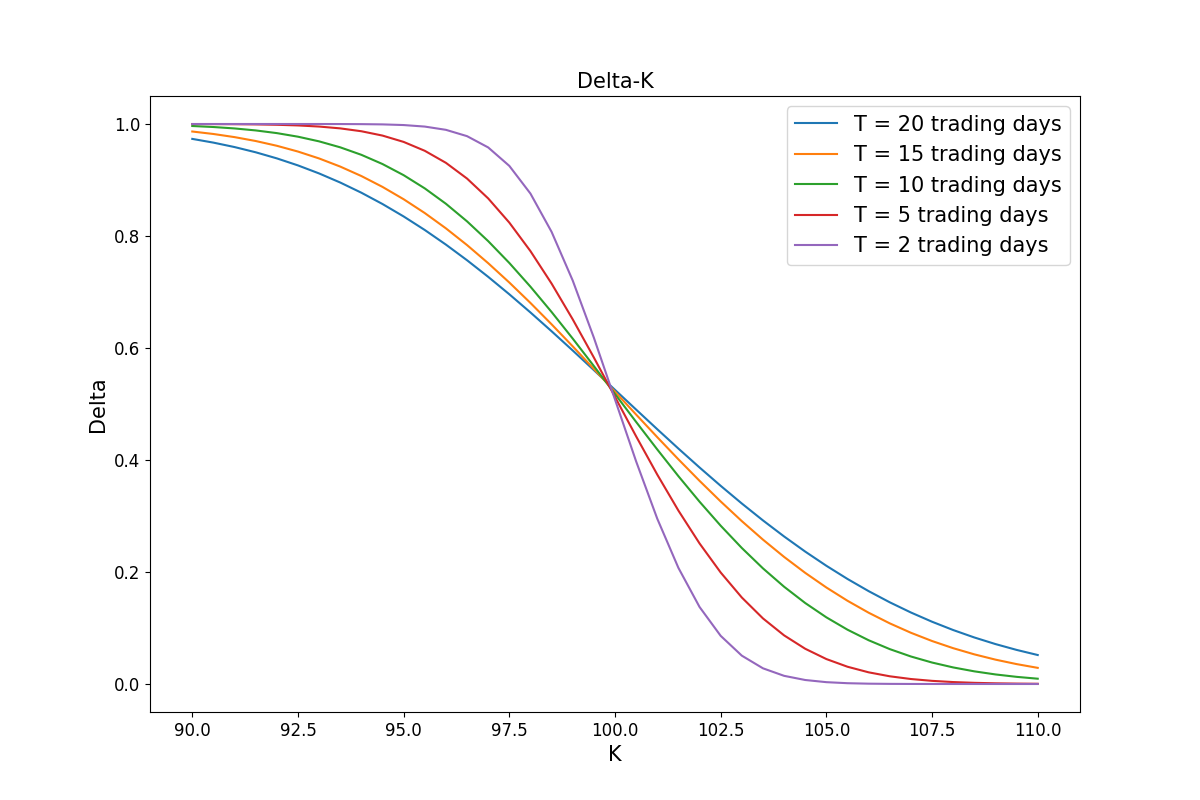
\includegraphics[width=12cm, height=8cm]{theory/delta_K.png}
  \caption[这里将出现在插图索引中]
    {看涨期权Delta与K和T的关系}
  \label{fig:delta_k}
\end{figure}

\begin{figure}[!htp]
  \centering
  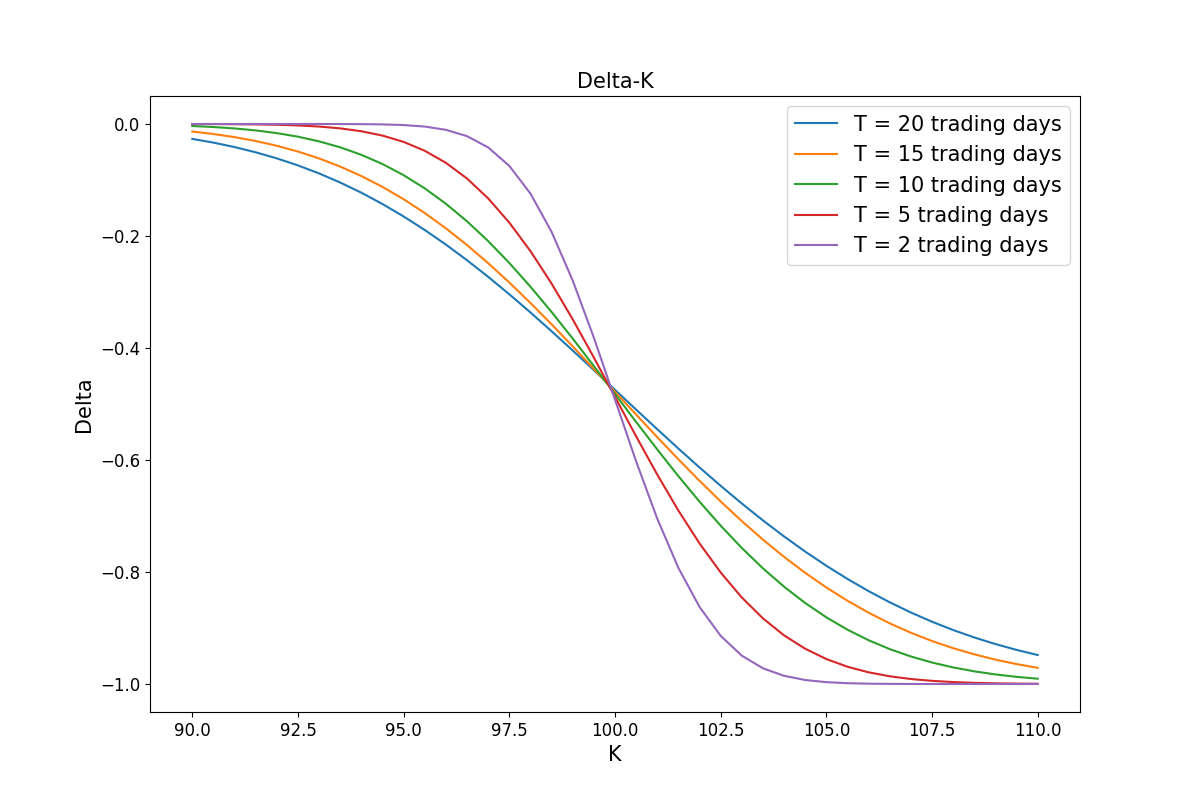
\includegraphics[width=12cm, height=8cm]{theory/put_delta_K.png}
  \caption[这里将出现在插图索引中]
    {看涨期权Delta与K和T的关系}
  \label{fig:put_delta_k}
\end{figure}

看涨期权的Delta值与行权价K和到期剩余时间T的关系如图\ref{fig:delta_k}所示,看跌期权的Delta值与行权价K和到期剩余时间T的关系如图\ref{fig:put_delta_k}所示。对于看涨期权来说,Delta始终为正,并且行权价K越高,Delta的绝对值越低;对于看跌期权来说,Delta始终为负,并且行权价K越高,Delta的绝对值越高,这其实可以从Delta的性质得到直观的理解。以看涨期权为例,Delta的计算公式为$N(d_1)$,与$N(d_2)$非常接近,而$N(d_2)$代表了在到期日标的价格达到K以上的概率,即看涨期权在到期日被行权的概率。因此,行权价K越高,看涨期权在到期日被行权的概率越低,Delta的绝对值越低。


\section{模拟方法}

在动态对冲研究中,模拟方法主要应用在资产价格路径的模拟上。关于资产价格路径的模拟,常用的有蒙特卡洛(Monte Carlo)方法和拟蒙特卡洛(Quasi-Monte Carlo)方法。蒙特卡洛方法是数值模拟中最为常用的方法,它实际上是这一类模拟方法的总称。本文所说的蒙特卡洛方法是一个相对狭义的概念,是指通过生成随机(random)或伪随机(pseudo-random)序列,模拟一个随机事件的可能情况,进而用频率来估计概率的方法。根据大数定律,若想有效地应用蒙特卡洛方法,需要较多的模拟的次数。在本文的研究中,我们并不直接考察每一次模拟的结果,而是对每一次的结果的一个函数进行求期望的操作,这一期望即为蒙特卡洛积分。设模拟次数为N,根据中心极限定理,蒙特卡洛积分的收敛速度为$O(N^{-\frac{1}{2}})$。蒙特卡洛的优势在于,其收敛速度独立于积分的维数。这一特点也使得其鲁棒性非常强,可以适用于很多高维的问题。然而,这一鲁棒性的代价是相对较慢的收敛速度。若要将误差的标准差大小的小数点向后移一位,需要将模拟次数提升为的100倍。

虽然蒙特卡洛方法鲁棒性较好,但是其对计算时间要求较高,因此本文最初希望可以找到一种收敛速度更快同时又不失鲁棒性的方法。我们考察了拟蒙特卡洛方法。拟蒙特卡洛方法使用低差异序列(low discrepancy sequence)进行模拟,经典的低差异序列包括Halton序列、Sobol序列和Faure序列。差异(discrepancy)是用来形容均匀性(uniformity)的,低差异序列比伪随机序列更接近均匀分布。与蒙特卡洛方法使用线性同余法等方法通过生成伪随机序列来试图模仿随机数的性质不同,低差异序列实际上是确定性的序列,并且其具有一定的自相关性来降低差异。因此拟蒙特卡洛方法只能用在蒙特卡罗积分问题上,使用其进行优化或单纯考察其模拟的结果是无意义的。拟蒙特卡洛模拟的收敛速度是$O((logN)^{d}N^{-1})$,其中d为模拟的维数。从这一收敛速度可以看出,当模拟次数N相对于维数d很大时,可以获得接近$O(N^{-1})$的收敛速度。然而,当d增长时,N需要以指数速度增长,以维持相应的收敛速度。如果N不足够大的话,拟蒙特卡洛模拟的收敛速度会慢于蒙特卡洛模拟的收敛速度。正如Caflisch(1998)指出的,高维性会很大程度上限制拟蒙特卡洛模拟的有效性。具体到本文的研究上,由于动态对冲是一个路径依赖的问题,因此其对应的维数即为标的资产价格路径模拟的频数,这一维数通常会很高(大于50)。在这样高维的模拟下,拟蒙特卡洛模拟效果将不如蒙特卡洛模拟。因此,在之后的研究中,本文将使用蒙特卡洛模拟生成资产价格序列。

当然,蒙特卡洛模拟可以通过方差减少技术来加快收敛速度,这一速度上的提高通常是通过减小$O(N^{-\frac{1}{2}})$项的系数,而并不会将速度提升一个量级,因此,对于这一技术,本文将不深入进行讨论,亦不会在应用中有所体现。关于拟蒙特卡洛模拟在高维情况下表现较差的问题,Wang和Sloan(2008)给出了一个解决方法,他们使用了一个新的计算差异的算法,使得拟蒙特卡洛方法在高维时的表现优于或至少不弱于蒙特卡洛方法。对于这一算法的细节、实现及应用,本文亦不进行讨论,而是将其作为未来可能的改进方向。

在确定了模拟使用的方法后,我们只是得到了生成参数为$(0,1)$的均匀分布的随机数的方式。获得了这一随机数后,可以使用正态分布的逆变换获得正态分布的随机数。之后,基于标的资产符合几何布朗运动的假设,生成价格序列。

%# -*- coding: utf-8-unix -*-
%%==================================================
%% chapter01.tex for SJTU Master Thesis
%%==================================================

%\bibliographystyle{sjtu2}%[此处用于每章都生产参考文献]
\chapter{模拟研究}
\label{chap:analysis}

\section{案例背景}

随着我国经济的发展,我国市场与全球市场联系的越来越紧密,各类商品的市场化程度不断升高,我国实体企业在原材料或产成品的价格上的风险意识也逐渐增强,使用衍生产品对冲风险的需求与日俱增。期权作为一种衍生产品,在风险对冲上有着诸多的优势,可以满足企业对价格风险管理的需求。然而,我国场内期权市场刚刚起步,提供的场内期权产品从数量上或品种上难以满足这些企业的需求。因此,诸多期货公司和券商作为场外期权的交易商,通过场外市场为这些企业提供场外期权,帮助他们进行风险管理。

在场外期权市场中,交易商以提供流动性为主,通常处于净卖出期权的位置。并且,由于期权空头方的理论最大损失远大于期权多头方的理论最大损失,对于期权空头的对冲是交易商通常更为关心的。在之后的研究中,我们将以一家期货公司面临的模拟案例的形式,主要对期权空头方的动态对冲进行分析。

A公司是全国知名的发电集团,以火力发电为主,对动力煤有稳定的需求。某日,A公司下属某发电厂欲于60个交易日后购入动力煤100万吨。该公司管理层经过讨论认为,应使用衍生品工具对冲这批动力煤未来价格上涨的风险。然而,由于近期动力煤价格不稳定,未来价格存在着一定的下行空间。因此,公司不希望直接使用期货锁定动力煤价格,以至于会在动力煤价格发生大幅下跌时仍以之前锁定的、相对较高的价格购入。基于以上考量,A公司决定向B期货公司购入看涨期权进行对冲。假设动力煤现货价格为100元/吨,每手期权对应1吨动力煤,期权执行价100元,无风险利率为每年3\%,动力煤收益率的波动率为每年20\%,期权期限为60个交易日。使用BS模型,可以得出该期权价格约为每张4.24413元。B期货公司在出售这些看涨期权后,面临对冲问题。公司决定使用动态对冲的方法来对冲暴露的期权空头。

\section{研究方法}

根据上文的分析,动态对冲的具体执行逻辑如下:在初始时刻,根据期权头寸暴露的Delta,买卖相应数量的标的资产,并记录相应的现金成本。若为买入标的资产,则现金成本为正;若为卖出标的资产,现金成本为负。之后每个交易日,根据累计的现金成本,使用无风险利率计算当日的利息支出或收入,加总到现金成本中。之后进行再平衡条件的判断,若满足再平衡条件(达到了确定的再平衡时刻或组合的Delta的绝对值超过了设定的Delta阈值),则进行对组合的再平衡,将组合的Delta暴露调整为0,并类似地记录现金成本,直到到期日结束。到期日结束后,根据期权的行权情况,计算现金上的支出或收入,记入现金成本。最后,将总现金成本折现回初始日期,得到对冲成本。若有交易成本的话,只需在买卖标的资产时对应扣减相应的现金成本即可。

在对动态对冲结果的评价上,我们使用三个指标:期望对冲成本、相对对冲波动率和平均再平衡次数。对冲成本期望为模拟结果中对冲成本的平均值,对冲成本期望越小,说明场外期权空头方以此策略对冲的期望成本越小,策略越优。相对对冲波动为标准化后的对冲成本的标准差,具体计算方法为模拟结果中对冲成本的标准差除以期权的理论价格,相对对冲波动越小,说明场外期权空头方以此策略对冲的成本的波动越小,对于风险厌恶型的空头方来说策略越优。再平衡次数则会影响到交易成本的计算,同时也会带来隐性的操作成本。一般认为其他指标相同的情况下,再平衡次数越少,策略越优。同时,我们也会考察对冲成本的偏度,以对动态对冲策略的尾部风险有所认识。

基于以上期权的基本参数以及动态对冲的执行逻辑和结果评价指标,我们使用蒙特卡洛模拟的方法,进行了四十万次模拟。根据蒙特卡洛模拟的收敛速度,最终得到的一阶矩的误差应当在0.0005量级,本节之后所有的数值上的比较和结论均以此误差范围为前提。我们分别模拟了固定时点对冲策略和固定Delta区间对冲策略的对冲效果,将首先考察无交易费用时动态对冲的结果,以对动态对冲的结果有一个初步的、直观的认识,之后再加入不同的交易成本,对比得出交易成本对动态对冲的影响。最后,我们将基于模拟结果,讨论动态对冲策略和参数的选择问题,试图找出最优的对冲策略及其对应的参数。

\section{无交易费用时的动态对冲}

\subsection{固定时点动态对冲}

在固定时点动态对冲中,我们选取再平衡时间间隔分别为1天、3天、5天、10天和15天,对冲结果如下

\begin{table}[htbp]
  \centering
  \caption{无交易费用时固定时点动态对冲结果}
  \label{tab:fixed_time_0}
  \begin{tabular}{cccccc}
    \toprule
    再平衡时间间隔 & 1 & 3 & 5 & 10 & 15 \\
    \midrule
    期望对冲成本 & 4.24392 & 4.24806 & 4.25002 & 4.25724 & 4.25955 \\
    对冲成本标准差 & 0.42881 & 0.73248 & 0.93660 & 1.30162 & 1.57070 \\
    相对对冲波动率 & 0.10104 & 0.17259 & 0.22068 & 0.30669 & 0.37009 \\
    平均再平衡次数 & 59.00000 & 19.00000 & 11.00000 & 5.00000 & 3.00000 \\
    对冲成本偏度 & 0.20244 & 0.31600 & 0.39032 & 0.52075 & 0.60554 \\
    \bottomrule
  \end{tabular}
\end{table}

\begin{figure}[htb]
  \centering
  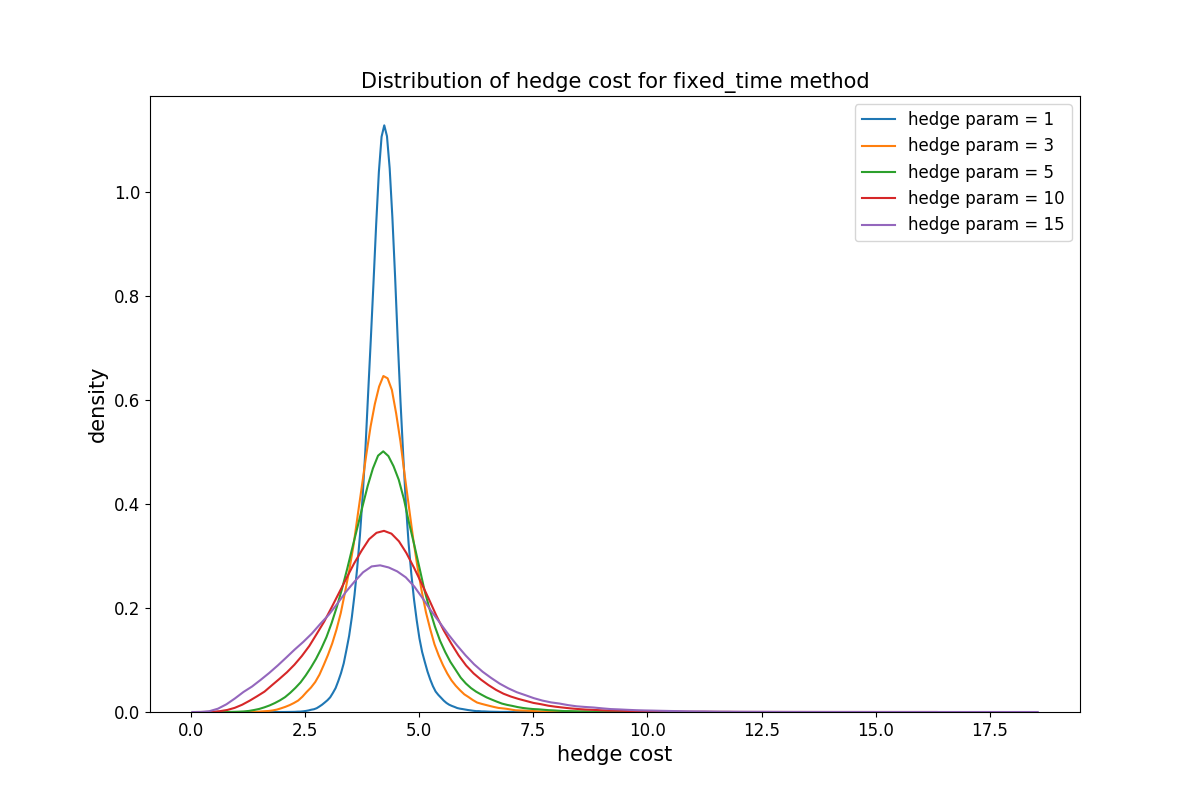
\includegraphics[width=12cm, height=8cm]{analysis/fixed_time_0_400000.png}
  \caption[这里将出现在插图索引中]
    {无交易费用时固定时点动态对冲对冲成本分布}
  \label{fig:fixed_time_0}
\end{figure}

从表\ref{tab:fixed_time_0}中,我们可以看出,随着再平衡频率的提高,对冲成本逐渐向BS模型计算出的理论价格收敛,并且相对对冲波动率逐渐减小,说明场外期权空头方的风险逐渐减小,最终的对冲成本变得更加"确定",对冲效果逐渐提高。这与BS模型的推导中的极限思想也是符合的。如果再平衡频率可以无限地提高,即再平衡时间间隔趋向于0,则期望对冲成本将依概率收敛到根据BS模型计算出的理论价格。虽然再平衡时间间隔为1天时的相对对冲波动率最低,对冲成本也最低,1天的再平衡时间间隔此时策略的最优参数,但是,其再平衡次数也达到了59次,若存在交易成本的话,频繁的再平衡将导致的交易成本的增加,这可能会提高对冲成本,使得其最终的期望对冲成本高于频率更低的情况。

图\ref{fig:fixed_time_0}展示了不同再平衡时间间隔下,对冲成本的分布情况。对冲成本的分布整体上呈现出右偏的特点。再平衡时间间隔越长时,对冲成本偏度越大,尾部风险较高,这可以从期权收益不对称的角度解释,同时也与动态对冲的具体的执行逻辑有关。Delta上的动态对冲在操作上其实是一个追涨杀跌的过程,最终的对冲成本取决于买入或卖出标的资产过程中标的资产的平均成交价格。随着到期日的临近,Gamma逐渐升高,由于再平衡时间较长,在两个再平衡时点之间如果标的价格出现了较强的单边趋势,则对冲组合的Delta相对于0的偏离值将会急剧增大,导致下一次再平衡时空头方需要以较高的价格买入大量标的资产对组合进行对冲。相比之下再平衡频率较高的情况,可以在标的出现单边趋势的过程中逐渐买入标的资产,最终标的资产的平均成交价格会相对较低,带来更低的对冲成本。因此,随着再平衡频率的提高,该动态对冲策略的尾部风险也会逐渐降低。

\subsection{固定Delta区间动态对冲}

在固定Delta区间动态对冲中,我们选取Delta阈值分别为0.03、0.05、0.1、0.15和0.2,对冲结果如下

\begin{table}[htbp]
  \centering
  \caption{无交易费用时固定Delta区间动态对冲结果}
  \label{tab:fixed_interval_0}
  \begin{tabular}{cccccc}
    \toprule
    Delta阈值 & 0.03 & 0.05 & 0.1 & 0.15 & 0.2 \\
    \midrule
    期望对冲成本 & 4.24618 & 4.24841 & 4.25352 & 4.26512 & 4.26066 \\
    对冲成本标准差 & 0.44593 & 0.48191 & 0.63572 & 0.83305 & 1.00841 \\
    相对对冲波动率 & 0.10507 & 0.11355 & 0.14979 & 0.19628 & 0.23760 \\
    平均再平衡次数 & 29.43722 & 20.25935 & 9.30494 & 5.20781 & 3.36678 \\
    对冲成本偏度 & 0.18198 & 0.14027 & 0.11910 & 0.22379 & 0.19918 \\
    \bottomrule
  \end{tabular}
\end{table}

\begin{figure}[htb]
  \centering
  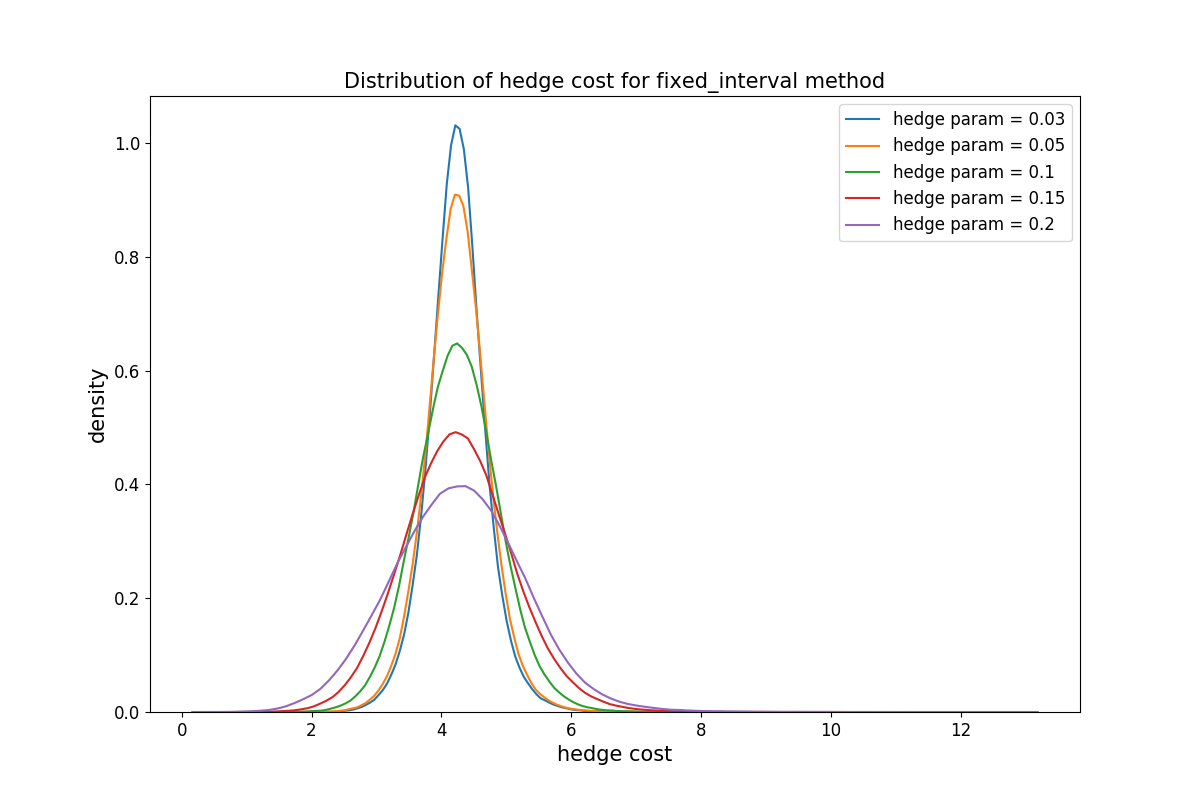
\includegraphics[width=12cm, height=8cm]{analysis/fixed_interval_0_400000.png}
  \caption[这里将出现在插图索引中]
    {无交易费用时固定Delta区间动态对冲对冲成本分布}
  \label{fig:fixed_interval_0}
\end{figure}

从表\ref{tab:fixed_interval_0}中,我们可以看出,随着Delta阈值的减小,对冲成本逐渐向BS模型计算出的理论价格收敛,并且相对对冲波动率逐渐减小,说明场外期权空头方的风险逐渐减小,最终的对冲成本变得更加"确定",对冲效果逐渐提高。类似的,Delta阈值为0.03时,对冲效果最好,但是此时的再平衡次数也最多。图\ref{tab:fixed_interval_0}中对冲成本的分布同样呈现出右偏的特点。但是,与固定时点对冲不同的是,随着Delta阈值的减小(对冲次数的增加),对冲成本偏度并没有出现递减的趋势。

\begin{table}[htbp]
  \centering
  \caption{无交易费用时固定Delta区间动态对冲结果}
  \label{tab:compare_two_0}
  \begin{tabular}{cccccc}
    \toprule
    Delta阈值/再平衡时间间隔 & 0.03/1 & 0.05/3 & 0.1/5 & 0.15/10 & 0.2/15 \\
    \midrule
    期望对冲成本百分比差异 & 0.05344\% & 0.00842\% & 0.08244\% & 0.18559\% & 0.02614\% \\
    相对对冲波动率绝对差异 & 0.40336\% & -5.90379\% & -7.08918\% & -11.04047\% & -13.24857\% \\
    \bottomrule
  \end{tabular}
\end{table}

将表\ref{tab:fixed_interval_0}和表\ref{tab:fixed_time_0}中平均再平衡次数最接近的结果进行对比,得到表\ref{tab:compare_two_0}。从该表中,我们发现在平均再平衡次数相差不大时(后四组结果),固定Delta区间对冲策略的期望对冲成本略高于固定时点对冲策略的期望对冲成本。这可以从两者在再平衡时需要对冲的Delta的值的分布得到解释。虽然两者对冲再平衡次数近似,但是对于固定Delta区间对冲来说,它每次再平衡时需要对冲的Delta一定会超过Delta阈值,因此其每次买入或卖出标的资产的量存在一个下界;而对于固定时点对冲,每次再平衡时需要对冲的Delta的绝对值不存在这样一个下界。因此在再平衡次数近似的情况下,前者的期望对冲成本会较高。同时,基于这一分析,固定Delta区间对冲对组合Delta的暴露控制的更好,因此其在相对对冲波动率的绝对数值上有很大提升。

再对比Delta阈值为0.03和再平衡时间间隔为1天的结果,两组结果的期望对冲成本和相对对冲波动率都差异不大,但是前者的平均再平衡次数在29次左右,而后者的再平衡次数达到了59次,这说明在有交易成本时,固定时点对冲的总对冲成本可能会高于固定Delta区间对冲。同时,固定Delta区间对冲策略的对冲成本偏度整体要小于固定时点对冲策略的对冲成本偏度。以上对比分析说明,在无交易成本时,固定Delta区间对冲策略的再平衡时点选择更为有效,其对冲效果要优于固定时点对冲策略,并且可以更好地减小尾部风险。

\section{有交易费用时的动态对冲}

在上一节,我们考察了无交易费用时,固定Delta区间对冲策略和固定时点对冲策略的对冲效果。在两个策略的分析中,我们都得出了再平衡次数越多,期望对冲成本越低,相对对冲波动率越低,对冲效果越好的结论。然而,在加入了交易费用后,再平衡次数越多,额外的交易成本也越多,因此对冲效果的比较结果可能会有所改变。本节我们将考察交易费用对对冲效果的影响。

我们采用固定比例的交易费用,分别选取0。02\%、0.05\%、0.08\%和0.1\%四个水平的交易成本,与上一节类似地进行动态对冲的模拟,模拟结果参见附录\ref{app:sim_fee_result}。我们将对表\ref{tab:fixed_time_0.02}到表\ref{tab:fixed_interval_0.1}的结果进行对比分析。

\subsection{交易费用对期望对冲成本的影响}

\begin{figure}[htb]
  \centering
  \subcaptionbox{固定时点动态对冲}[12cm]
    {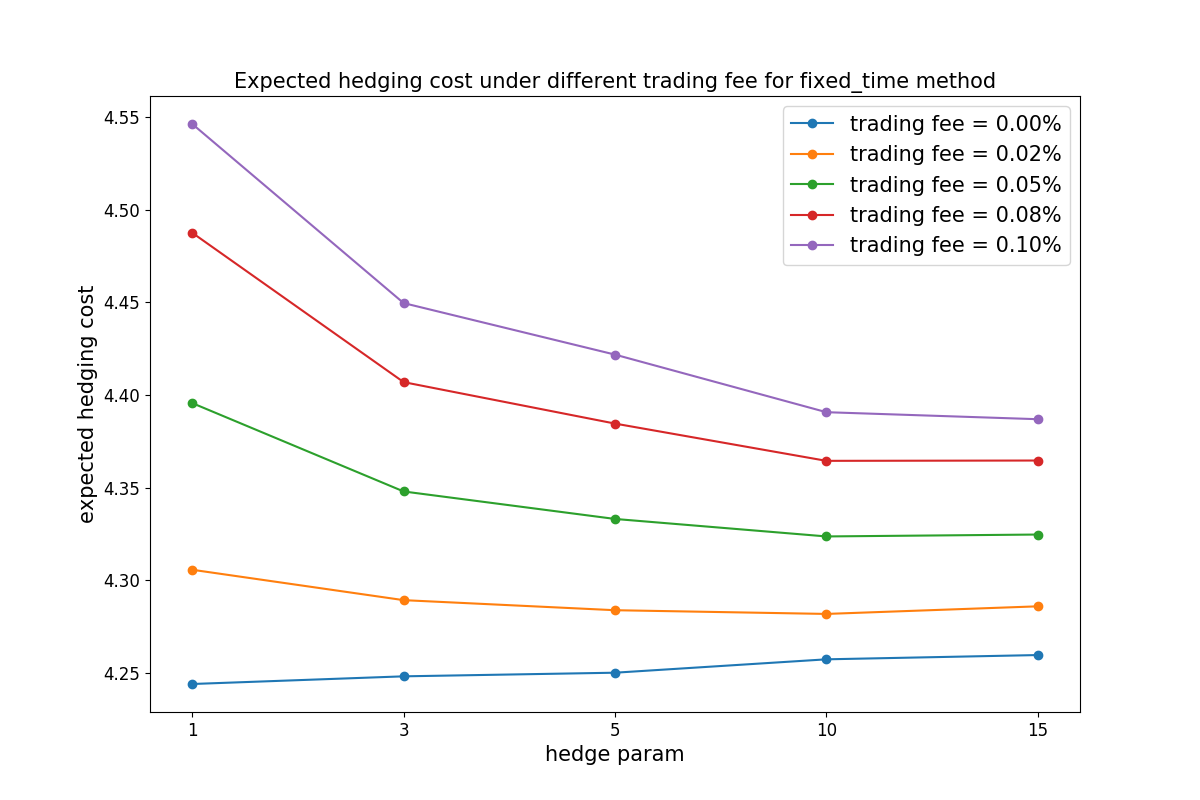
\includegraphics[width=12cm]{analysis/hedge_fee_fixed_time.png}}
  \hspace{0.5cm}
  \subcaptionbox{固定Delta区间动态对冲}[12cm]
    {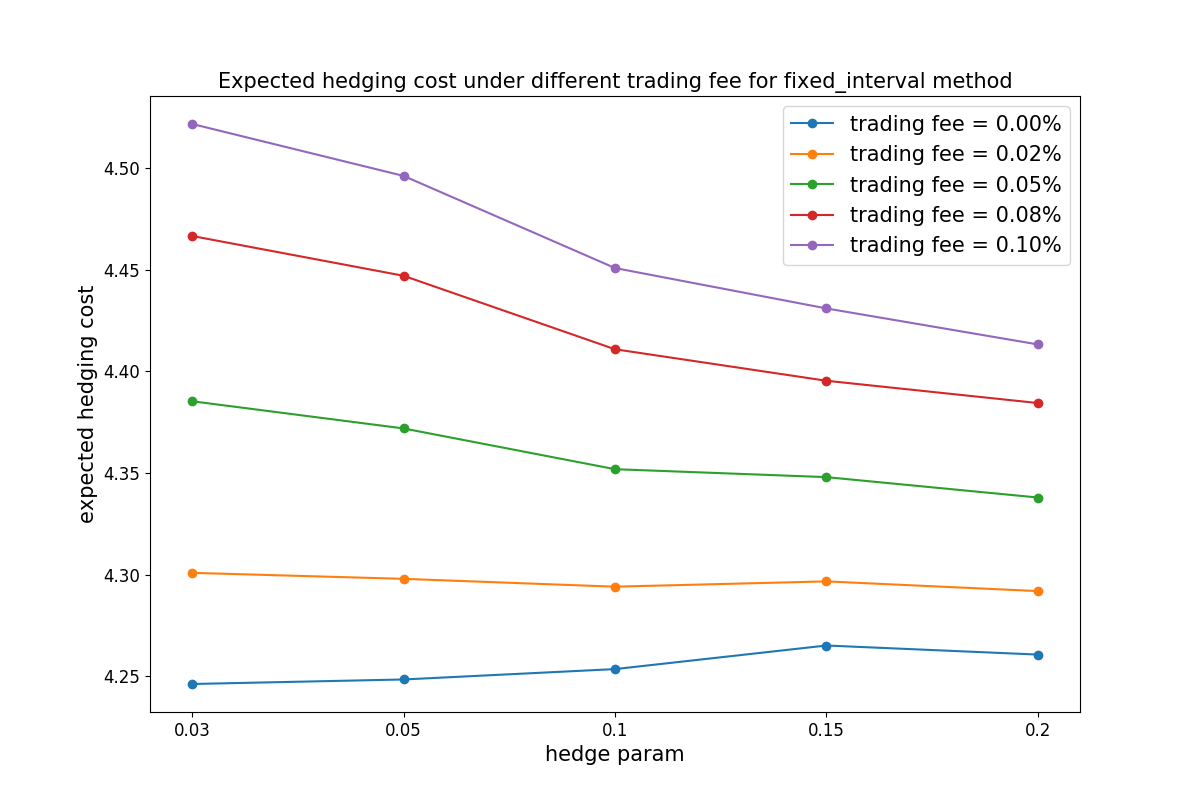
\includegraphics[width=12cm]{analysis/hedge_fee_fixed_interval.png}}
    \caption[这里将出现在插图索引中]
    {交易费用对期望对冲成本的影响}
  \label{fig:hedge_fee}
\end{figure}

图\ref{fig:hedge_fee}展示了不同交易费用对期望对冲成本的影响。引入交易费用将会增加期望对冲成本,其他条件相同的情况下,交易费用越高,期望对冲成本越高。

通过相同策略下每个表内结果的比较,我们发现随着平均再平衡次数的增加,期望对冲成本也基本上呈现出增加的趋势,但是并不严格单调。例如对于固定时点对冲策略,在交易费用较小时,存在一个再平衡时间间隔,其期望对冲成本为极值点,当再平衡时间间隔从该时间间隔增加或减小时,期望对冲成本总是增加。由于较长的再平衡时间间隔将带来较大的对冲误差,从而增加对冲成本,同时平均再平衡次数的增加也会增加交易费用从而对冲成本,因此在两者的共同作用下,将存在一个极值点,使其期望对冲成本最小。当交易费用较大时,其影响将占主要部分,此时期望对冲成本将会更严格地随平均再平衡次数递增。

通过不同策略,相同交易费用设定下结果的比较,我们发现平均再平衡次数相差不大的结果中(每张表的后四组结果),固定Delta区间对冲策略的期望对冲成本略高于固定时点对冲策略的期望对冲成本,幅度大概在0.5\%到1\%左右(相对于期权理论价格),这一期望对冲成本增加的原因在上一节有所提及。实际上,类似的平均再平衡次数下,固定Delta区间对冲策略中期望对冲成本的增加是对相对对冲波动率降低的一个“惩罚”,也正是由于该策略可以更有效地选择再平衡时刻,因此才会有更高的期望对冲成本和更低的相对对冲波动率。再比较每张表的第一组结果,我们发现在相对对冲波动率相差不大的情况下,固定Delta区间对冲策略下的期望对冲成本略低于固定时点对冲策略的期望对冲成本,这说明在该组结果的比较中,固定Delta区间对冲策略更优。

\subsection{交易费用对相对对冲波动率的影响}

\begin{figure}[htb]
  \centering
  \subcaptionbox{固定时点动态对冲}[12cm]
    {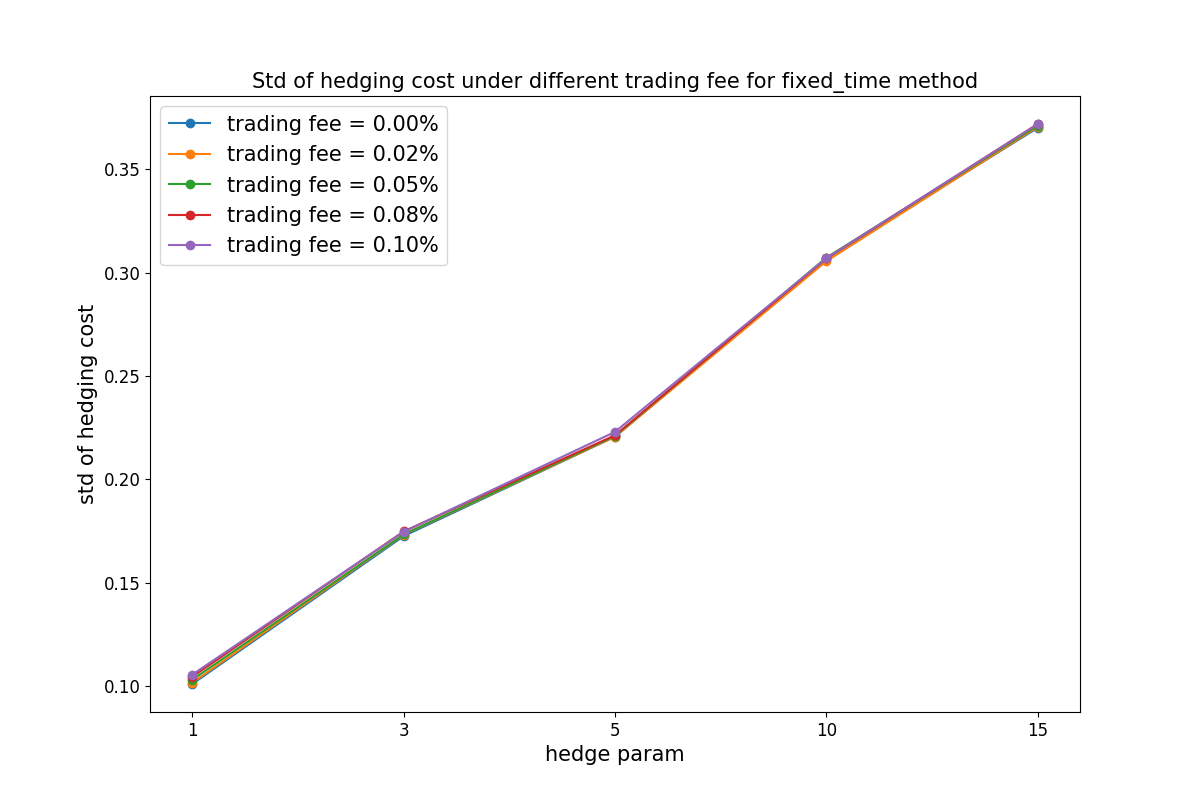
\includegraphics[width=12cm]{analysis/hedge_std_fixed_time.png}}
  \hspace{0.5cm}
  \subcaptionbox{固定Delta区间动态对冲}[12cm]
    {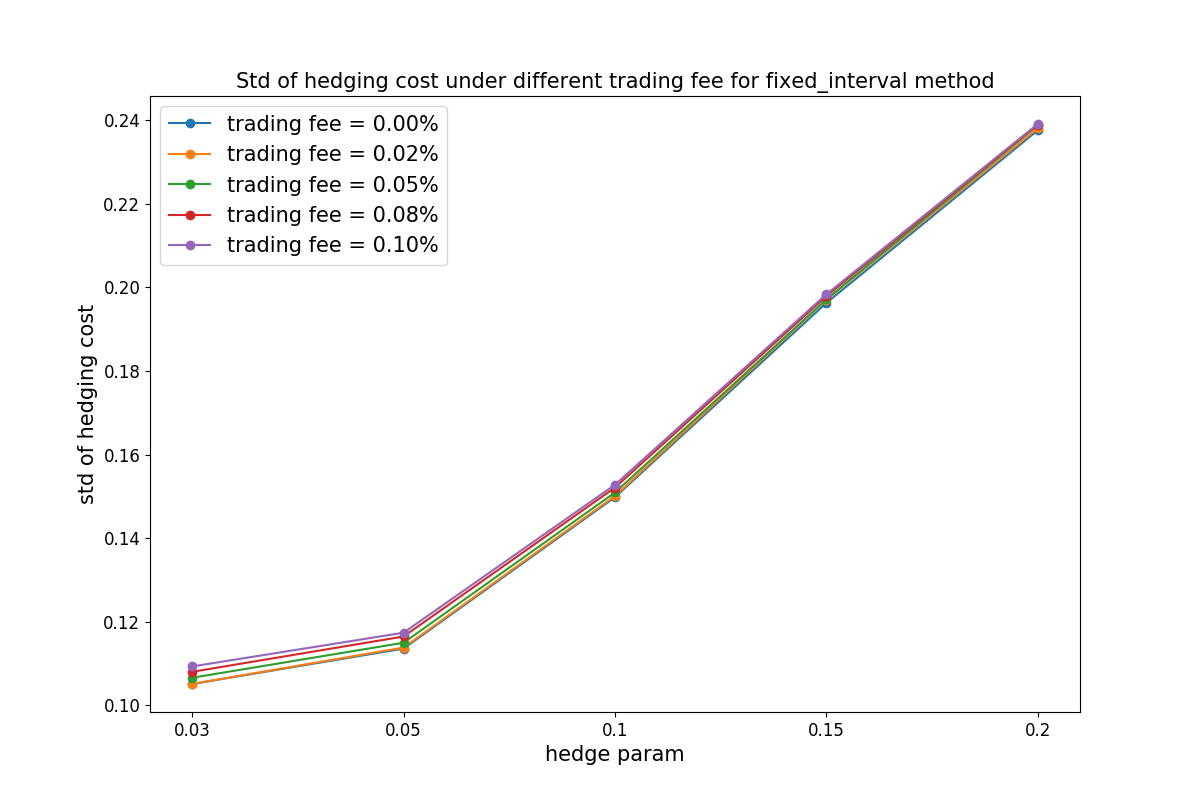
\includegraphics[width=12cm]{analysis/hedge_std_fixed_interval.png}}
    \caption[这里将出现在插图索引中]
    {交易费用对相对对冲波动率的影响}
  \label{fig:hedge_std}
\end{figure}

图\ref{fig:hedge_std}展示了不同交易费用对相对对冲波动率的影响。我们发现不同交易费用下,两个策略的相对对冲波动率水平和无交易费用时相差不大,但是基本呈现出随交易费用的增加而增加的趋势,这一现象在固定Delta对冲策略中Delta阈值为0.03时最为明显。由于我们使用的是成比例的交易费用,因此交易费用的引入相当于是成比例地增加了对冲成本,最终使得相对对冲波动率也会按照一定比例有所增加。

\subsection{交易费用对对冲成本偏度的影响}

\begin{figure}[htb]
  \centering
  \subcaptionbox{固定时点动态对冲}[12cm]
    {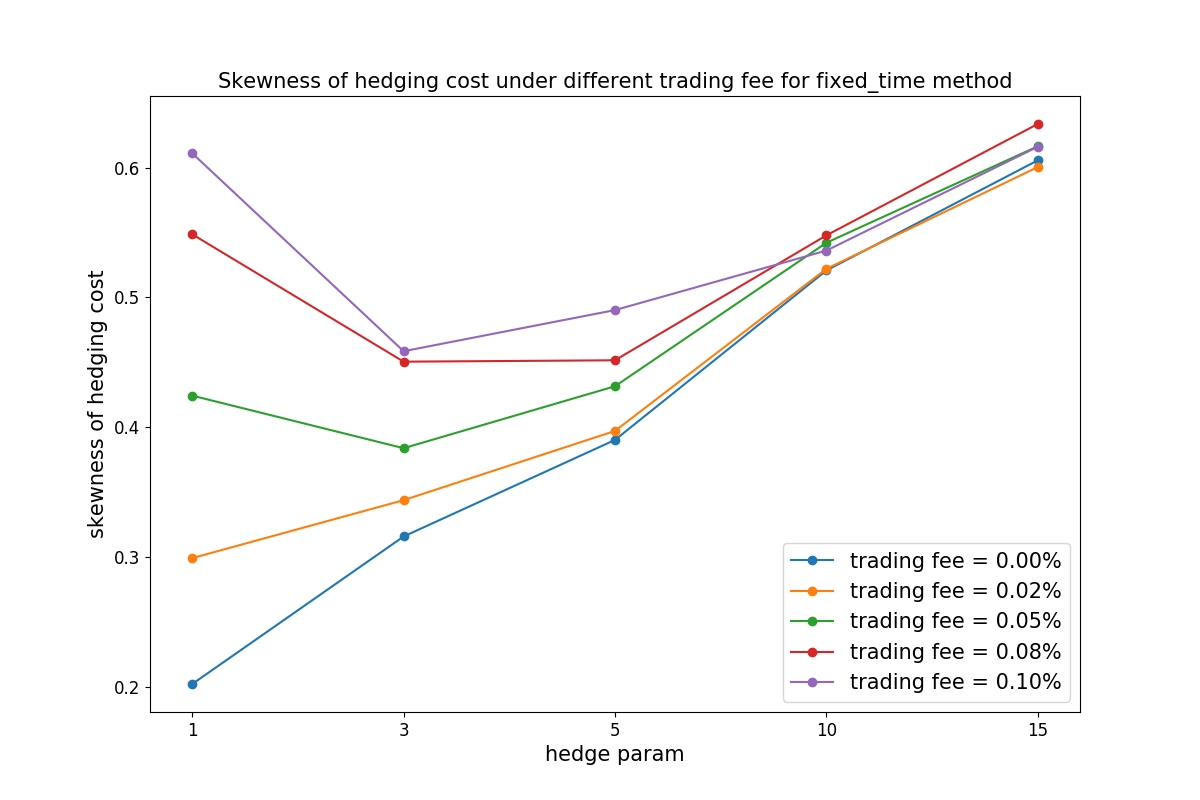
\includegraphics[width=12cm]{analysis/hedge_skew_fixed_time.png}}
  \hspace{0.5cm}
  \subcaptionbox{固定Delta区间动态对冲}[12cm]
    {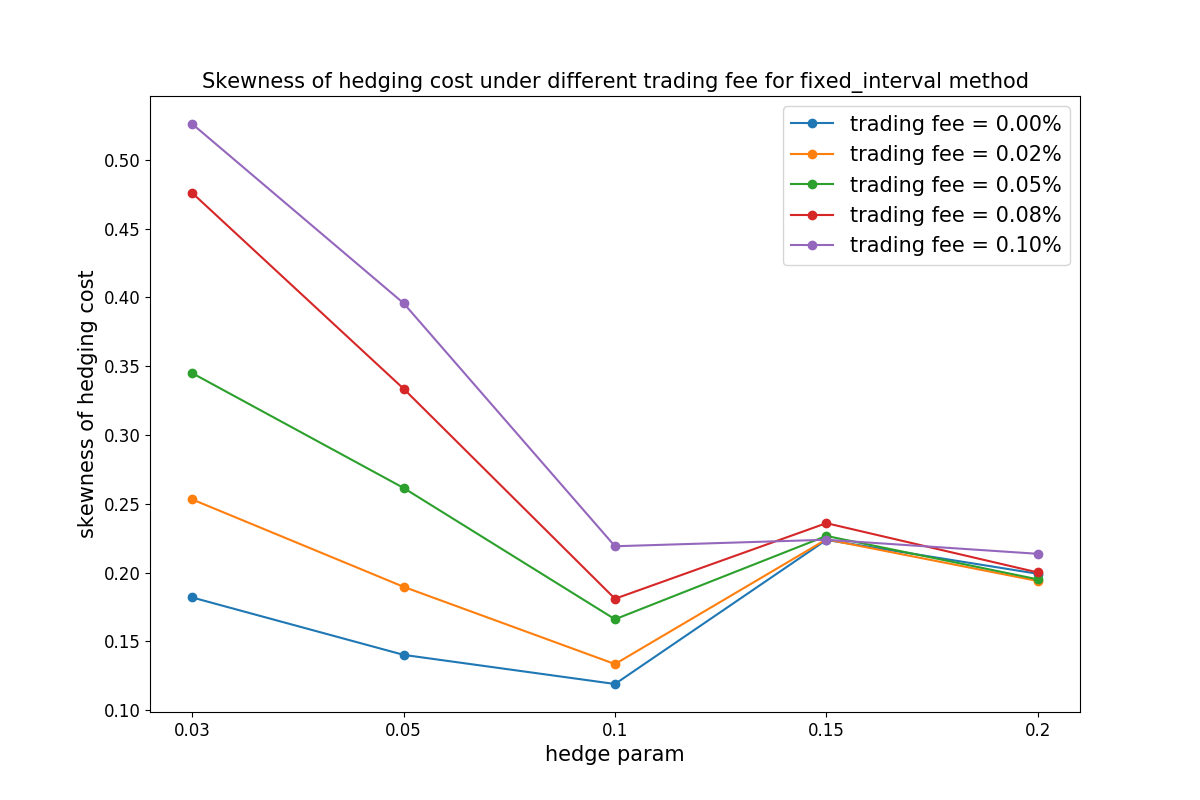
\includegraphics[width=12cm]{analysis/hedge_skew_fixed_interval.png}}
    \caption[这里将出现在插图索引中]
    {交易费用对对冲成本偏度的影响}
  \label{fig:hedge_skew}
\end{figure}

图\ref{fig:hedge_skew}展示了不同交易费用对对冲成本偏度的影响。我们发现交易费用的引入将显著地提升对冲成本的偏度。考察无交易费用时,处于右尾上的对冲成本对应的对冲操作。我们之前提到,这些对冲成本较高的情况一般是出现了较强的、不利的单边趋势。在这种情况下,场外期权空头方每次再平衡都需要买入(针对本章设定的卖出看涨期权情况)标的资产,交易费用的加入会带来更高的对冲成本;对于均值附近的对冲成本对应的动态对冲操作,这些情况下标的资产一般呈现震荡走势,空头方不需要在标的资产市场上进行数额较大的操作,额外的交易费用带来的对冲成本也会相对较小。因此,交易成本的引入将加剧原有对冲成本分布的右偏程度。并且,我们发现平均再平衡次数越高,对冲成本偏度的增加越明显,甚至会使得对冲成本偏度和平均再平衡次数的关系出现反转。这说明再平衡次数的增加带来的交易成本的增加对偏度影响要大于再平衡次数较少时对冲不精确的影响。

\section{动态对冲策略和参数选择}
\label{utility}

在上两节中,我们考察了有交易费用和无交易费用时,两个动态对冲策略的模拟结果。我们初步分析了对冲结果的期望对冲成本、相相对对冲波动率和对冲成本偏度,对不同参数下不同策略在这三个指标上的表现和变化特点有了初步的了解。本节我们将参考均值-方差效用函数,具体探讨如何根据以上指标,制定出动态对冲策略和参数选择的评判标准。

均值-方差效用函数的具体形式如下
\begin{equation}
  U=\mu+\frac{1}{2}\lambda\sigma^2
\end{equation}
其中,$\mu$为年化期望收益率,$\sigma$为年化收益率标准差,$\lambda$为风险偏好系数。当$\lambda$为负时,说明投资者是风险厌恶的,$\lambda$的绝对值越大,投资者的风险厌恶程度越高。本文假设场外期权交易商为风险厌恶者。

首先,我们定义对冲成本率为
\begin{equation}
  u=-(\frac{hc}{prc}-1)
\end{equation}
其中,$hc$为对冲成本,$prc$为期权的理论价格,$T_{total}$为期权的总期限。将其乘以一个年化系数即得到了年化对冲成本率。年化对冲成本率实际上代表了某种对冲策略下,相对于BS模型设定下的理想状态年化后的额外对冲成本。基于对冲成本率的概念,则$\mu$为年化期望对冲成本率,$\sigma$为年化对冲成本率标准差。利用之前提到的动态对冲的评价指标,我们可以得到适用于动态对冲策略分析的$\mu$和$\sigma$
\begin{equation}
  \mu=-(\frac{E[hc]}{prc}-1)\frac{252}{T_{total}}
  \label{eq:mu}
\end{equation}
\begin{equation}
  \sigma=rhv\sqrt{\frac{252}{T_{total}}}
  \label{eq:sigma}
\end{equation}
其中,$rhv$为相对对冲波动率,$E[hc]$为期望对冲成本。关于式\ref{eq:mu}和式\ref{eq:sigma}的具体推导见附录\ref{app:eq}。

我们以交易费用为万分之五为例,分析在这一对冲得分标准下,动态对冲策略和参数的选择。首先,固定时点对冲策略和固定Delta区间对冲策略的$\mu$和$\sigma$如下

\begin{table}[htbp]
  \centering
  \caption{动态对冲策略的$\mu$和$\sigma$}
  \label{tab:compare_two_0}
  \begin{tabular}{cccccc}
    \toprule
    Delta阈值/再平衡时间间隔 & 0.03/1 & 0.05/3 & 0.1/5 & 0.15/10 & 0.2/15 \\
    \midrule
    固定时点对冲策略的$\mu$ & -0.14990 & -0.10269 & -0.08800 & -0.07865 & -0.07967 \\
    固定Delta区间动态对冲策略的$\mu$ & -0.13965 & -0.12642 & -0.10659 & -0.10273 & -0.09281 \\
    固定时点对冲策略的$\sigma$ & 0.21130 & 0.35532 & 0.45301 & 0.62981 & 0.76059 \\
    固定Delta区间对冲策略的$\sigma$ & 0.21840 & 0.23557 & 0.30927 & 0.40400 & 0.48942 \\
    \bottomrule
  \end{tabular}
\end{table}

\begin{figure}[htb]
  \centering
  \subcaptionbox{固定时点动态对冲}[12cm]
    {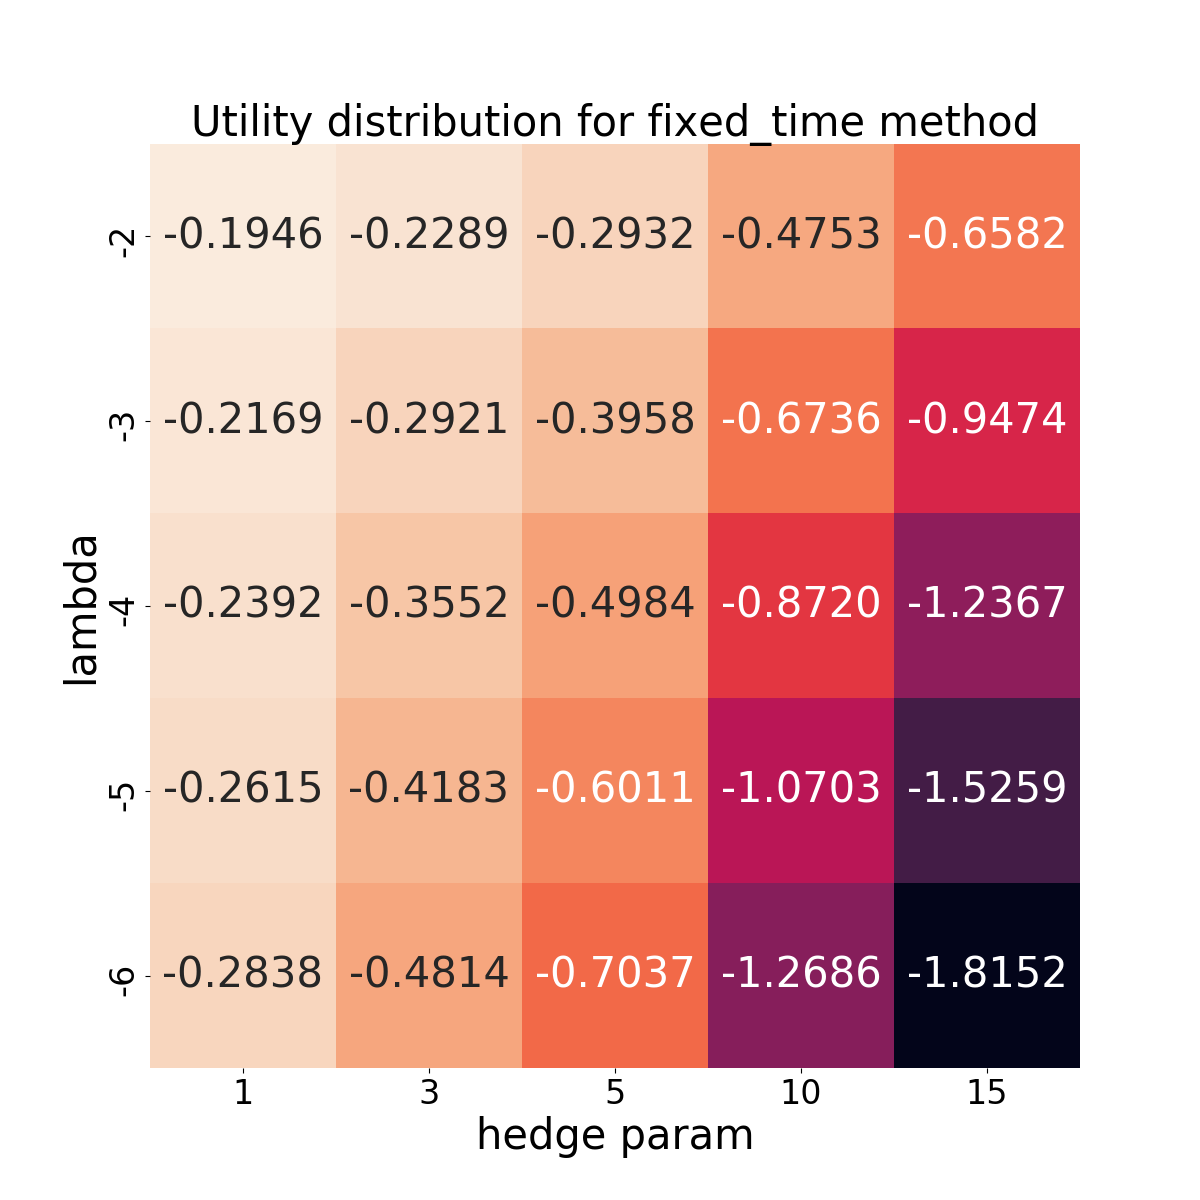
\includegraphics[width=7.5cm]{analysis/hedge_utility_fixed_time.png}}
  \hspace{0.5cm}
  \subcaptionbox{固定Delta区间动态对冲}[12cm]
    {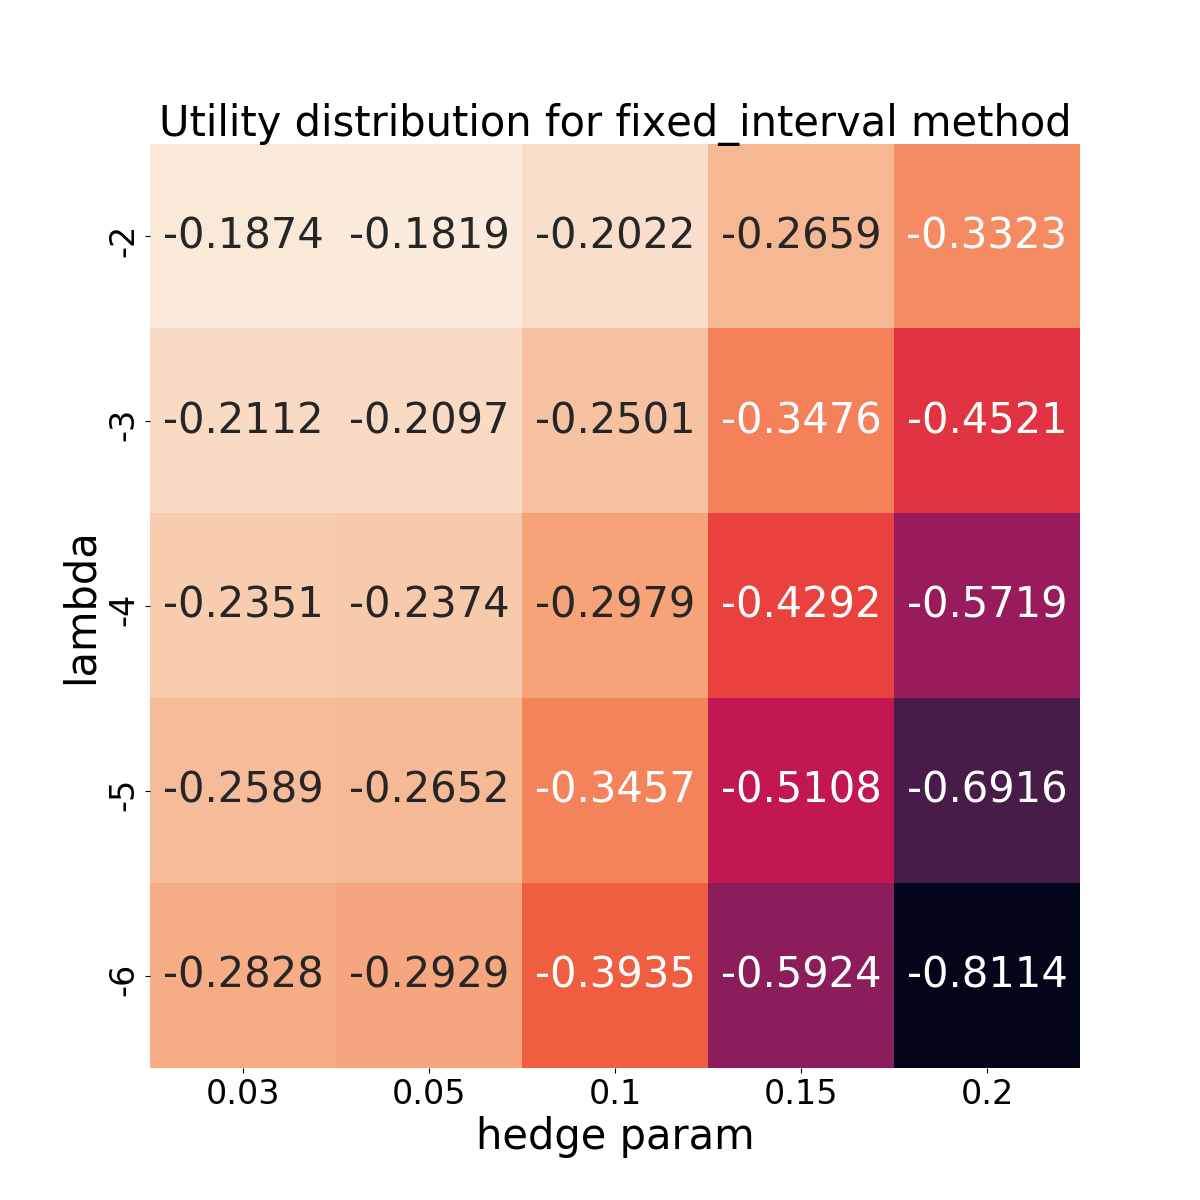
\includegraphics[width=7.5cm]{analysis/hedge_utility_fixed_interval.png}}
    \caption[这里将出现在插图索引中]
    {均值-方差对冲得分}
  \label{fig:hedge_utility}
\end{figure}

基于上述公式,我们设定$\lambda$为-2、-3、-4、-5和-6,计算得出两个策略的得分如图\ref{fig:hedge_utility}所示。从该图中可以看出,对于固定时点对冲策略,在固定$\lambda$值时,对冲得分总是和对冲参数呈负相关关系。这说明相比于对冲参数的改变带来的对冲成本的减少,这一评判标准认为其带来的在对冲成本波动率上的改进影响更大。因此,在给定的参数范围内,对于固定时点对冲策略,场外期权交易商应当选择再平衡时间间隔为1天。对于固定Delta区间对冲策略,结论大致与固定时点对冲相同。但是,我们发现在$\lambda$的绝对值小于或等于3时,Delta阈值为0.05的结果要优于Delta阈值为0。03的结果,当$\lambda$的绝对值大于3时,结果相反。这说明对于场外期权交易商而言,如果风险厌恶程度较低,则Delta阈值为0.05相对于0.03,在对冲成本上降低对最终对冲得分的影响效果要大于对冲成本波动率上的增加,交易商对期望对冲成本更为敏感;如果风险厌恶程度较高,则交易商会对对冲成本波动更为敏感,因此偏好Delta阈值为0.03的策略。但是总体上看,两个参数下策略表现相差不大。

横向对比固定时点对冲策略和固定Delta区间对冲策略,我们发现整体上来看固定Delta区间对冲策略的得分要高于固定时点对冲策略。这说明固定Delta区间对冲策略要优于固定时点对冲策略。并且,从两组策略对应位置的对冲得分差值随$\lambda$的变化中可以看出,场外期权交易商的风险厌恶程度越高,越偏好固定Delta区间对冲策略。

基于以上模拟研究,我们可以得出以下结论:场外期权交易商在对冲其看涨期权空头方向的暴露时,应当选择固定Delta区间对冲策略,具体阈值的选择取决于风险厌恶程度。

\section{本章小结}

本章以虚拟案例的形式,对动态对冲进行了模拟研究,主要考察动态对冲策略中各个参数以及交易成本对动态对冲结果的影响,同时对动态对冲的最优参数选择进行讨论。我们主要使用了期望对冲成本、相对对冲波动率和平均再平衡次数三个指标,也考察了对冲成本偏度。我们结合策略的操作特点对这些指标的表现进行了解释,并模仿均值-方差效用函数提出了一个动态对冲策略和参数选择的评判标准,同时基于这一标准对两个对冲策略在各个参数下的表现进行了评价,最终得出固定Delta区间对冲策略为更优的结论。在固定Delta区间策略中,具体阈值的选择取决于交易商的风险厌恶程度。

%# -*- coding: utf-8-unix -*-
%%==================================================
%% chapter01.tex for SJTU Master Thesis
%%==================================================

%\bibliographystyle{sjtu2}%[此处用于每章都生产参考文献]
\chapter{实证分析}
\label{chap:empirical}

\section{数据选取和处理}

我们选取Wind提供的动力煤指数(ZCFI.WI)作为标的资产价格序列进行实证分析。动力煤指数由每个动力煤合约按照持仓额加权平均计算得出.选择动力煤指数而非动力煤主连合约作为标的资产价格序列的原因是,动力煤主连合约在主力合约切换时会发生跳价,无法计算此时的收益率及其波动率。

我们选取时间区间为2013年12月25日至2019年4月23日的动力煤指数日收盘价格数据,动力煤指数对数收益率的分布和描述性统计如下

\begin{figure}[htb]
  \centering
  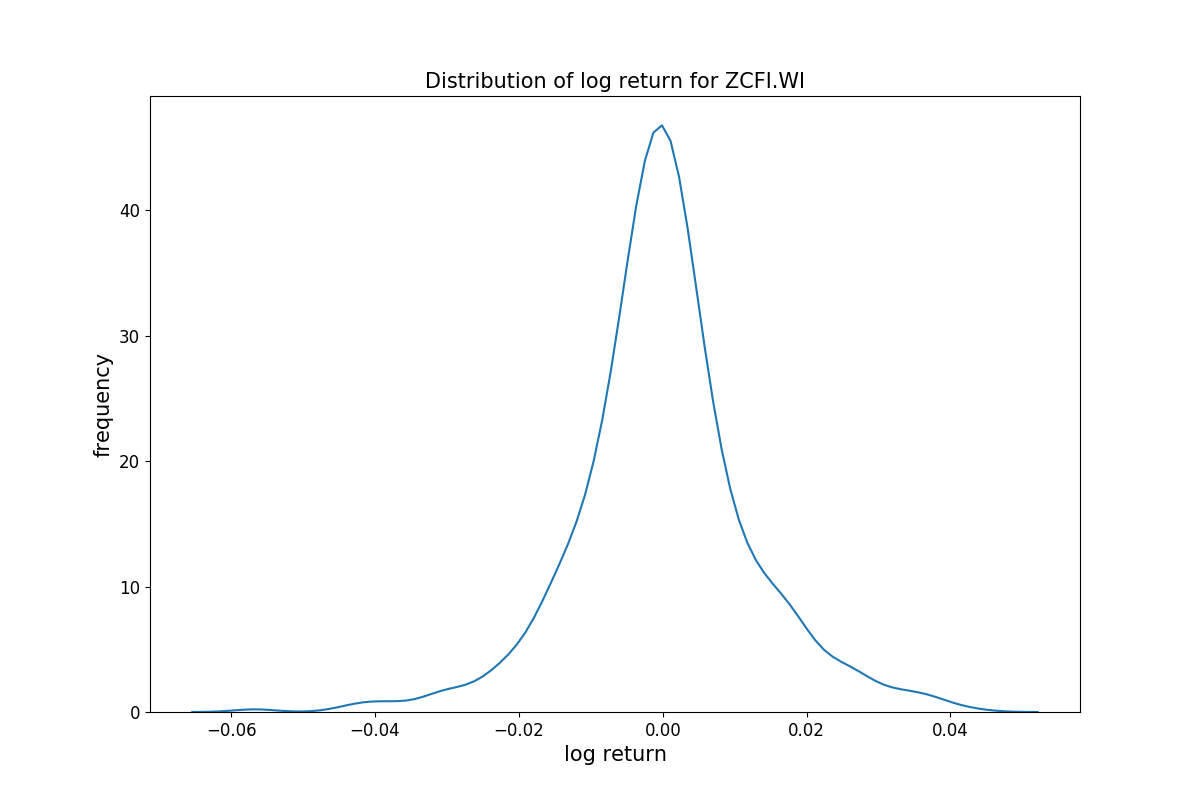
\includegraphics[width=12cm, height=8cm]{analysis/dist_ZCFI.png}
  \caption[这里将出现在插图索引中]
    {动力煤指数对数收益率分布}
  \label{fig:ZCFI_describe}
\end{figure}

\begin{table}[htbp]
  \centering
  \caption{动力煤指数对数收益率的描述性统计}
  \label{tab:ZCFI_describe}
  \begin{tabular}{cc}
    \toprule
    统计量 & 值 \\
    \midrule
    mean & 4.20435E-05 \\
    std & 1.21309E-02 \\
    variance & 1.47159E-04 \\
    min & -5.67394E-02 \\
    max & 4.34607E-02 \\
    5\% & -1.96002E-02 \\
    25\% & -5.77001E-03 \\
    50\% & -1.99533E-04 \\
    75\% & 5.64455E-03 \\
    95\% & 2.06669E-02 \\
    iqr & 1.14146E-02 \\
    kurtosis & 2.09724E+00 \\
    skewness & -6.06696E-02 \\
    \bottomrule
  \end{tabular}
\end{table}

从图\ref{fig:ZCFI_describe}和表\ref{tab:ZCFI_describe}中可以看出,动力煤指数对数收益率存在着左偏的现象。经过Jarque-Bera检验,p值近似为0,说明动力煤指数对数收益率序列不服从正态分布,我们将在之后具体分析这一分布特点对其对冲结果的影响。

在动态对冲的实证研究中,需要确定计算Delta时使用的隐含波动率。我们将分别采用滚动计算的窗宽为60的历史波动率和滚动计算的$\beta$为0.94、最小窗宽为60的EWMA波动率作为这一波动率的估计,并比较两者对应的结果差异。两个波动率随时间变化的趋势如图\ref{fig:vol_ZCFI}。从图中可以看出,历史波动率相对于EWMA波动率更为平滑。计算得出历史波动率的均值约为0.18064,EWMA波动率的均值约为0.17919。

\begin{figure}[htb]
  \centering
  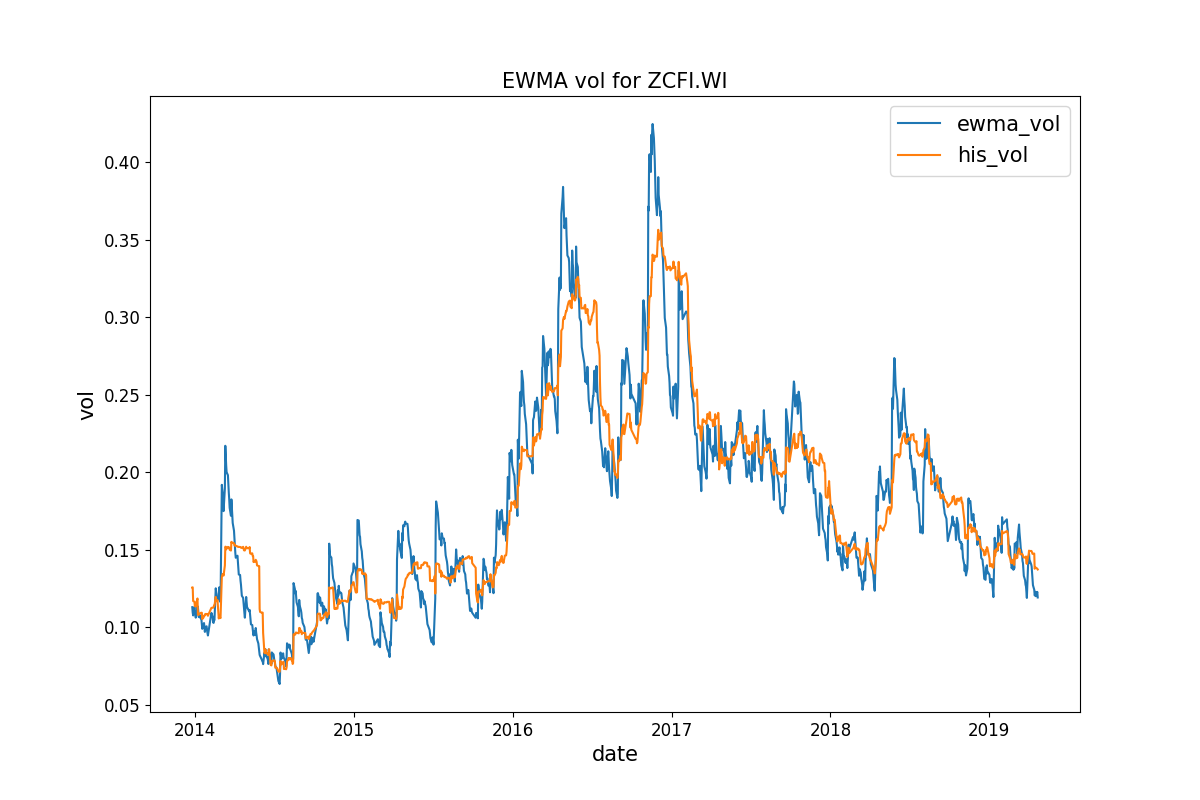
\includegraphics[width=12cm, height=8cm]{analysis/vol_ZCFI.png}
  \caption[这里将出现在插图索引中]
    {动力煤指数对数收益率的波动率}
  \label{fig:vol_ZCFI}
\end{figure}

\section{模型确立}

在上一章中,我们介绍了模拟研究中动态对冲操作的基本逻辑和评判指标。使用实际数据进行研究与模拟研究的原理类似,但是受数据特点的影响,我们在具体操作和结果评价上都有所调整。在动态对冲的具体操作中,我们在原数据上以60+1为窗宽滚动采样进行动态对冲策略的回测(第一个数据用于对冲组合的初始化)。在估计波动率时,我们使用第一个数据对应的历史波动率或EWMA波动率作为动态对冲中计算Delta时使用的隐含波动率。在确定行权价格时,我们使用第一个数据对应的动力煤指数价格为行权价。其他变量的设定与上一章相同。

在对冲结果的评价上,上一章以对冲成本为出发点,使用了期望对冲成本、相对对冲波动率和平均再平衡次数三个指标,也考察了对冲成本的波动率。本章由于滚动使用实际数据进行动态对冲分析,每个滚动窗口对应的隐含波动率均不相同,因此每段对应的期权理论价格也不相同,难以采用对冲成本进行评价。回顾第\ref{utility}小节,我们介绍并推导了年化对冲成本率的概念。年化对冲成本率是一个标准化的指标,一般为负值,可以用于不同隐含波动率、不同行权价格下对冲成本的比较。因此,我们在实证研究中,对于每一个滚动窗口下的对冲结果计算对冲成本率,最后计算年化期望对冲成本率、年化对冲成本率标准差、平均再平衡次数和对冲成本率偏度,作为对对冲结果的评价。我们将以交易费用为万分之五为例,计算固定时点动态对冲策略和固定Delta区间动态对冲策略在实际数据上的表现。

\section{固定时点动态对冲}

在实际数据上进行固定时点动态对冲,使用历史波动率的结果如下

\begin{table}[htbp]
  \centering
  \caption{使用历史波动率时固定时点动态对冲结果}
  \label{tab:fixed_time_5_his_vol_real}
  \begin{tabular}{cccccc}
    \toprule
    再平衡时间间隔 & 1 & 3 & 5 & 10 & 15 \\
    \midrule
    年化期望对冲成本率 & -0.21307 & -0.28222 & -0.30179 & -0.38262 & -0.58224 \\
    年化对冲成本率标准差 & 0.49910 & 0.60425 & 0.65314 & 0.66530 & 0.79351 \\
    平均再平衡次数 & 59.00000 & 19.00000 & 11.00000 & 5.00000 & 3.00000 \\
    对冲成本率偏度 & -1.26083 & -1.43039 & -1.82980 & -0.58411 & -0.72386 \\
    \bottomrule
  \end{tabular}
\end{table}

\begin{figure}[htb]
  \centering
  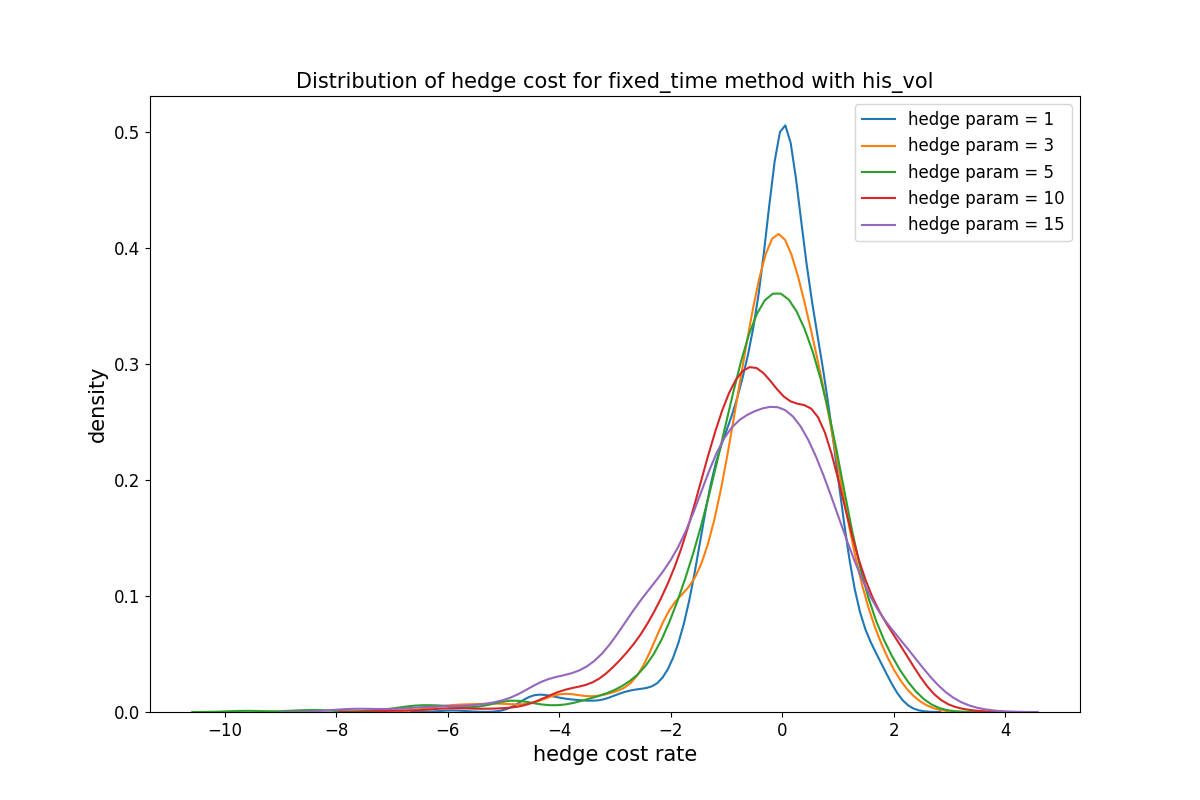
\includegraphics[width=12cm, height=8cm]{analysis/fixed_time_5_his_vol_real.png}
  \caption[这里将出现在插图索引中]
    {使用历史波动率时固定时点动态对冲年化对冲成本率分布}
  \label{fig:fixed_time_5_his_vol_real}
\end{figure}
使用EWMA波动率的结果如下

\begin{table}[htbp]
  \centering
  \caption{使用EWMA波动率时固定时点动态对冲结果}
  \label{tab:fixed_time_5_ewma_vol_real}
  \begin{tabular}{cccccc}
    \toprule
    再平衡时间间隔 & 1 & 3 & 5 & 10 & 15 \\
    \midrule
    年化期望对冲成本率 & -0.22197 & -0.29719 & -0.32270 & -0.42106 & -0.64521 \\
    年化对冲成本率标准差 & 0.50521 & 0.61185 & 0.66963 & 0.69798 & 0.85823 \\
    平均再平衡次数 & 59.00000 & 19.00000 & 11.00000 & 5.00000 & 3.00000 \\
    对冲成本率偏度 & -1.15463 & -1.30845 & -1.92706 & -0.56951 & -0.94468 \\
    \bottomrule
  \end{tabular}
\end{table}

\begin{figure}[htb]
  \centering
  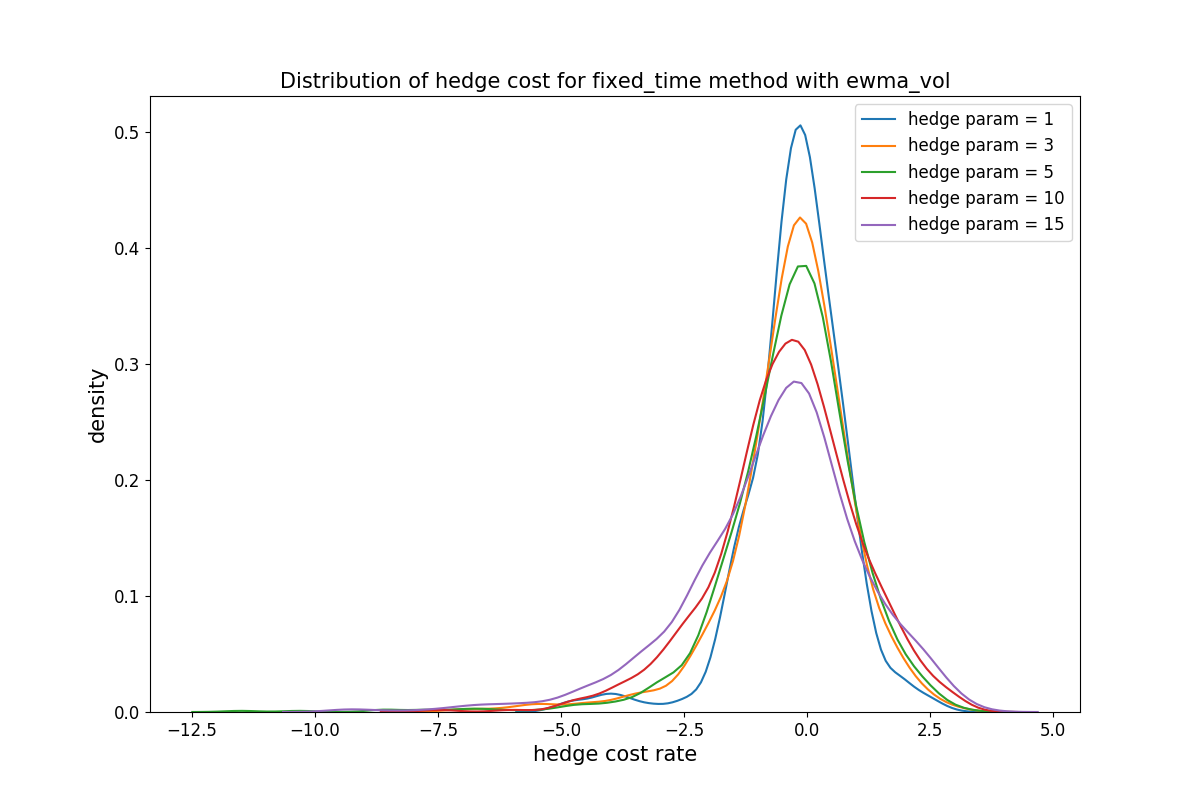
\includegraphics[width=12cm, height=8cm]{analysis/fixed_time_5_ewma_vol_real.png}
  \caption[这里将出现在插图索引中]
    {使用EWMA波动率时固定时点动态对冲年化对冲成本率分布}
  \label{fig:fixed_time_5_ewma_vol_real}
\end{figure}

首先,对比表\ref{tab:fixed_time_5_his_vol_real}和\ref{tab:fixed_time_5_ewma_vol_real},我们发现使用历史波动率时,年化期望对冲成本率的绝对值和年化对冲成本率标准差均低于使用EWMA波动率时的结果。年化期望对冲成本率较低是由于历史波动率的均值要高于EWMA波动率,因此使用历史波动率相当于是在复制了一个相对于EWMA波动率方法下有波动率溢价的期权。年化对冲波动率较低也是因为历史波动率的整体水平较高,在对冲时有一个更高的、与实际波动相关的时间价值来抵消一部分对冲成本,从而带来更低的在对冲成本上的波动。这说明在定价时合理地加入波动率溢价,可以提升对冲效果。因此,对于场外期权交易商而言,需要在基于历史数据的波动率之上加入一个溢价,以抵消对冲的额外成本以及降低对冲成本的波动,这也部分解释了场内期权市场中隐含波动率相对于标的历史波动率溢价的原因。

\begin{table}[htbp]
  \centering
  \caption{模拟研究中的固定时点动态对冲结果}
  \label{tab:fixed_time_5_sim}
  \begin{tabular}{cccccc}
    \toprule
    再平衡时间间隔 & 1 & 3 & 5 & 10 & 15 \\
    \midrule
    年化期望对冲成本率 & -0.14990 & -0.10269 & -0.08800 & -0.07865 & -0.07967 \\
    年化对冲成本率标准差 & 0.21130 & 0.35532 & 0.45301 & 0.62981 & 0.76059 \\
    平均再平衡次数 & 59.00000 & 19.00000 & 11.00000 & 5.00000 & 3.00000 \\
    对冲成本率偏度 & -0.42441 & -0.38394 & -0.43164 & -0.54209 & -0.61634 \\
    \bottomrule
  \end{tabular}
\end{table}

之后,将实证分析的结果同模拟研究的结果进行对比。表\ref{tab:fixed_time_5_sim}展示了固定时点对冲的相应指标结果。我们发现,从绝对数值上看,实证分析的结果中的年化期望对冲成本率、年化对冲成本率标准差和对冲成本率偏度均明显高于模拟研究的结果。这可以从以下几个方面得到解释:首先,动力煤指数收益率的分布与正态分布相差较大,由此会带来对冲成本在分布上的差异;其次,由于实际数据的数据量有限,滚动进行的回测结果的数量无法达到与模拟研究相同级别的收敛程度;最重要的一点是,我们使用的是期初固定的波动率,可能无法准确地预测未来动力煤指数的实际波动率,并且由于卖出期权收益的不对称性,动力煤指数在波动率上的波动(volatility of volatility)也会给对冲带来额外的成本。

从相对数值上看,我们发现实证分析的结果中,年化对冲成本率标准差随平均再平衡次数的变化关系与模拟研究保持一致。然而,年化期望对冲成本率的这一关系差异较大。随着平均再平衡次数的减少,年化期望对冲成本率增加。这说明在实际对冲操作中,对冲不精确带来的损失远大于对冲频繁带来的额外交易成本。这也启示我们当不能够准确预测波动率时,可以通过更加频繁地再平衡操作来降低对冲成本。同时,由于不同再平衡次数下,实证分析结果的年化期望对冲成本率相差较大,对对冲成本率偏度的数值也有一定的影响。

\section{固定Delta区间动态对冲}

在实际数据上进行固定Delta区间动态对冲,使用历史波动率的结果如下

\begin{table}[htbp]
  \centering
  \caption{使用历史波动率时固定Delta区间动态对冲结果}
  \label{tab:fixed_interval_5_his_vol_real}
  \begin{tabular}{cccccc}
    \toprule
    Delta阈值 & 0.03 & 0.05 & 0.1 & 0.15 & 0.2 \\
    \midrule
    年化期望对冲成本率 & -0.22378 & -0.22533 & -0.30528 & -0.36488 & -0.52749 \\
    年化对冲成本率标准差 & 0.49734 & 0.49510 & 0.52071 & 0.55105 & 0.62216 \\
    平均再平衡次数 & 22.68119 & 15.58111 & 7.23487 & 4.22760 & 2.92333 \\
    对冲成本率偏度 & -1.17149 & -1.15062 & -0.73235 & -0.51298 & -0.38667 \\
    \bottomrule
  \end{tabular}
\end{table}

\begin{figure}[htb]
  \centering
  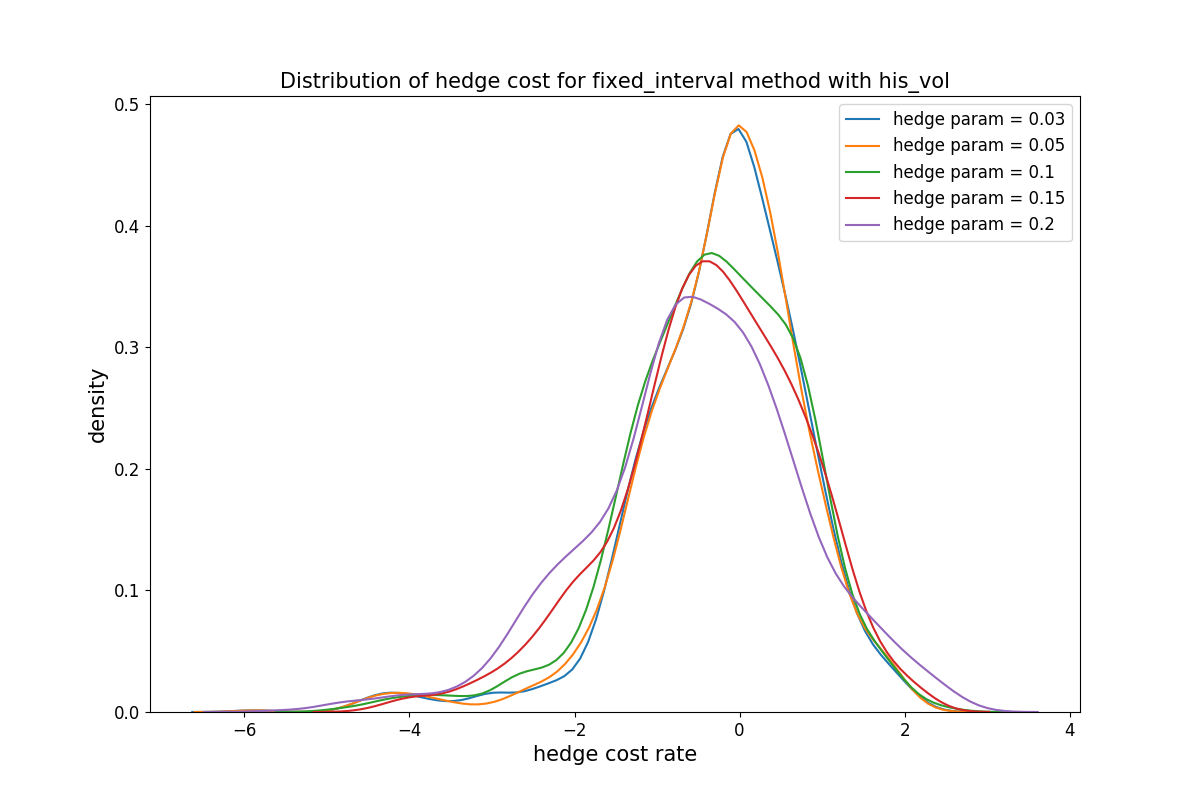
\includegraphics[width=12cm, height=8cm]{analysis/fixed_interval_5_his_vol_real.png}
  \caption[这里将出现在插图索引中]
    {使用历史波动率时固定Delta区间动态对冲年化对冲成本率分布}
  \label{fig:fixed_interval_5_his_vol_real}
\end{figure}
使用EWMA波动率的结果如下

\begin{table}[htbp]
  \centering
  \caption{使用EWMA波动率时固定Delta区间动态对冲结果}
  \label{tab:fixed_interval_5_ewma_vol_real}
  \begin{tabular}{cccccc}
    \toprule
    Delta阈值 & 0.03 & 0.05 & 0.1 & 0.15 & 0.2 \\
    \midrule
    年化期望对冲成本率 & -0.23541 & -0.22623 & -0.30755 & -0.41459 & -0.58979 \\
    年化对冲成本率标准差 & 0.50814 & 0.51192 & 0.53600 & 0.60002 & 0.67011 \\
    平均再平衡次数 & 22.58515 & 15.35916 & 7.29298 & 4.26715 & 2.93866 \\
    对冲成本率偏度 & -1.06379 & -1.03056 & -0.72411 & -0.50804 & -0.52199 \\
    \bottomrule
  \end{tabular}
\end{table}

\begin{figure}[htb]
  \centering
  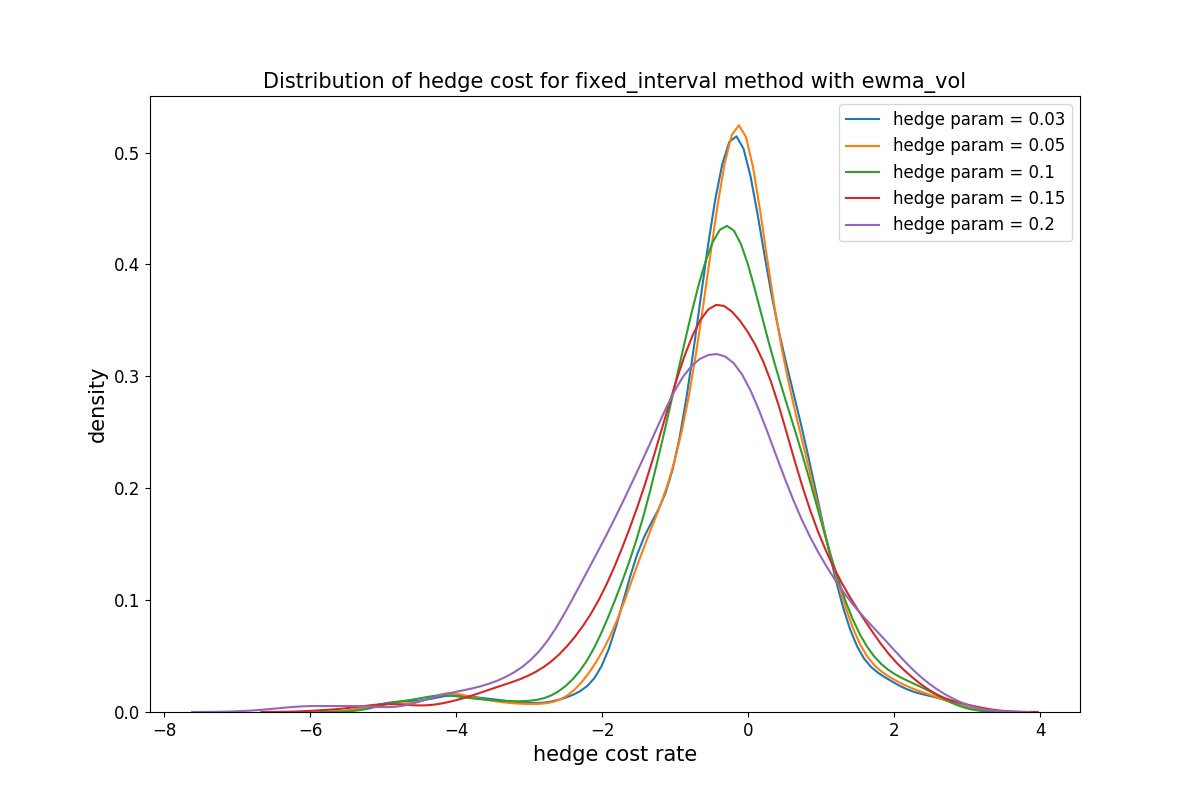
\includegraphics[width=12cm, height=8cm]{analysis/fixed_interval_5_ewma_vol_real.png}
  \caption[这里将出现在插图索引中]
    {使用EWMA波动率时固定Delta区间动态对冲年化对冲成本率分布}
  \label{fig:fixed_interval_5_ewma_vol_real}
\end{figure}

首先,对比表\ref{tab:fixed_interval_5_his_vol_real}和\ref{tab:fixed_interval_5_ewma_vol_real},结论与上一节类似。将本节结果与上一节的结果进行对比,我们发现固定Delta区间动态对冲的年化对冲成本率标准差整体上小于固定时点对冲,尤其是考虑到固定Delta区间动态对冲的平均再平衡次数明显较少,这说明在实际操作中,固定Delta区间动态对冲的再平衡操作更为高效。比较年化期望对冲成本率,固定Delta区间动态对冲策略下的结果从整体上看也明显较低。

然而,具体考察平均再平衡次数最高的结果,我们发现固定时点对冲策略的年化期望对冲成本率要低于固定Delta区间对冲策略的这一数值。这与上文提到的波动率估计不精确有关。由于波动率估计的不精确,在动态对冲过程中计算的Delta也难以反映对冲组合对标的价格真正的敏感性,导致在Delta阈值的判断并不能够像模拟研究中那样准确地描述风险暴露,从而降低了对冲效果。因此,在实际市场操作中,每日进行再平衡操作最终可以获得更低的对冲成本,其带来的更为精确的对冲效果可以弥补额外的交易费用。

\begin{table}[htbp]
  \centering
  \caption{模拟研究中的固定时点动态对冲结果}
  \label{tab:fixed_interval_5_sim}
  \begin{tabular}{cccccc}
    \toprule
    Delta阈值 & 0.03 & 0.05 & 0.1 & 0.15 & 0.2 \\
    \midrule
    年化期望对冲成本率 & -0.13965 & -0.12642 & -0.10659 & -0.10273 & -0.09281 \\
    年化对冲成本率标准差 & 0.21840 & 0.23557 & 0.30927 & 0.40400 & 0.48942 \\
    平均再平衡次数 & 29.40321 & 20.23523 & 9.30451 & 5.20708 & 3.37050 \\
    对冲成本率偏度 & -0.34495 & -0.26154 & -0.16613 & -0.22670 & -0.19515 \\
    \bottomrule
  \end{tabular}
\end{table}

表\ref{tab:fixed_interval_5_sim}展示了模拟研究中固定时点对冲的相应对冲结果。将实证分析的结果同模拟研究的结果进行对比,结论与上一节较为类似,在此不再赘述。

\section{动态对冲策略和参数选择}
\label{utility_real}

使用上一章提出的对冲得分指标,对实证分析的结果类似地做出评价,在此仅使用历史波动率下的结果。EWMA波动率下的结果参见附录\ref{app:utility_result_real}。

\begin{figure}[htb]
  \centering
  \subcaptionbox{固定时点动态对冲}[12cm]
    {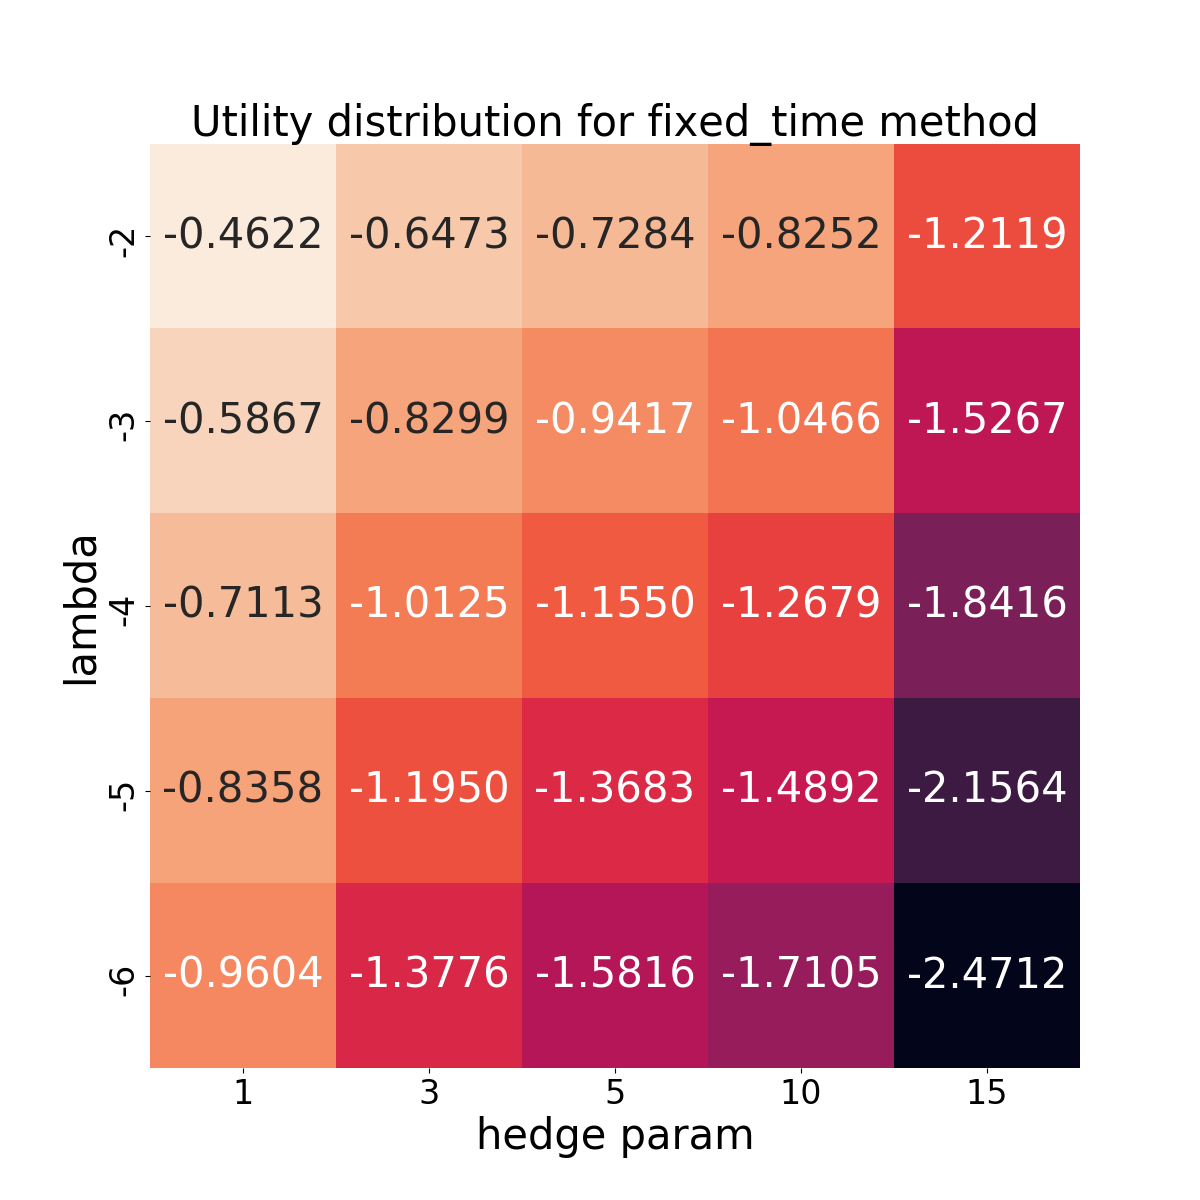
\includegraphics[width=7.5cm]{analysis/hedge_utility_real_fixed_time_his_vol.png}}
  \hspace{0.5cm}
  \subcaptionbox{固定Delta区间动态对冲}[12cm]
    {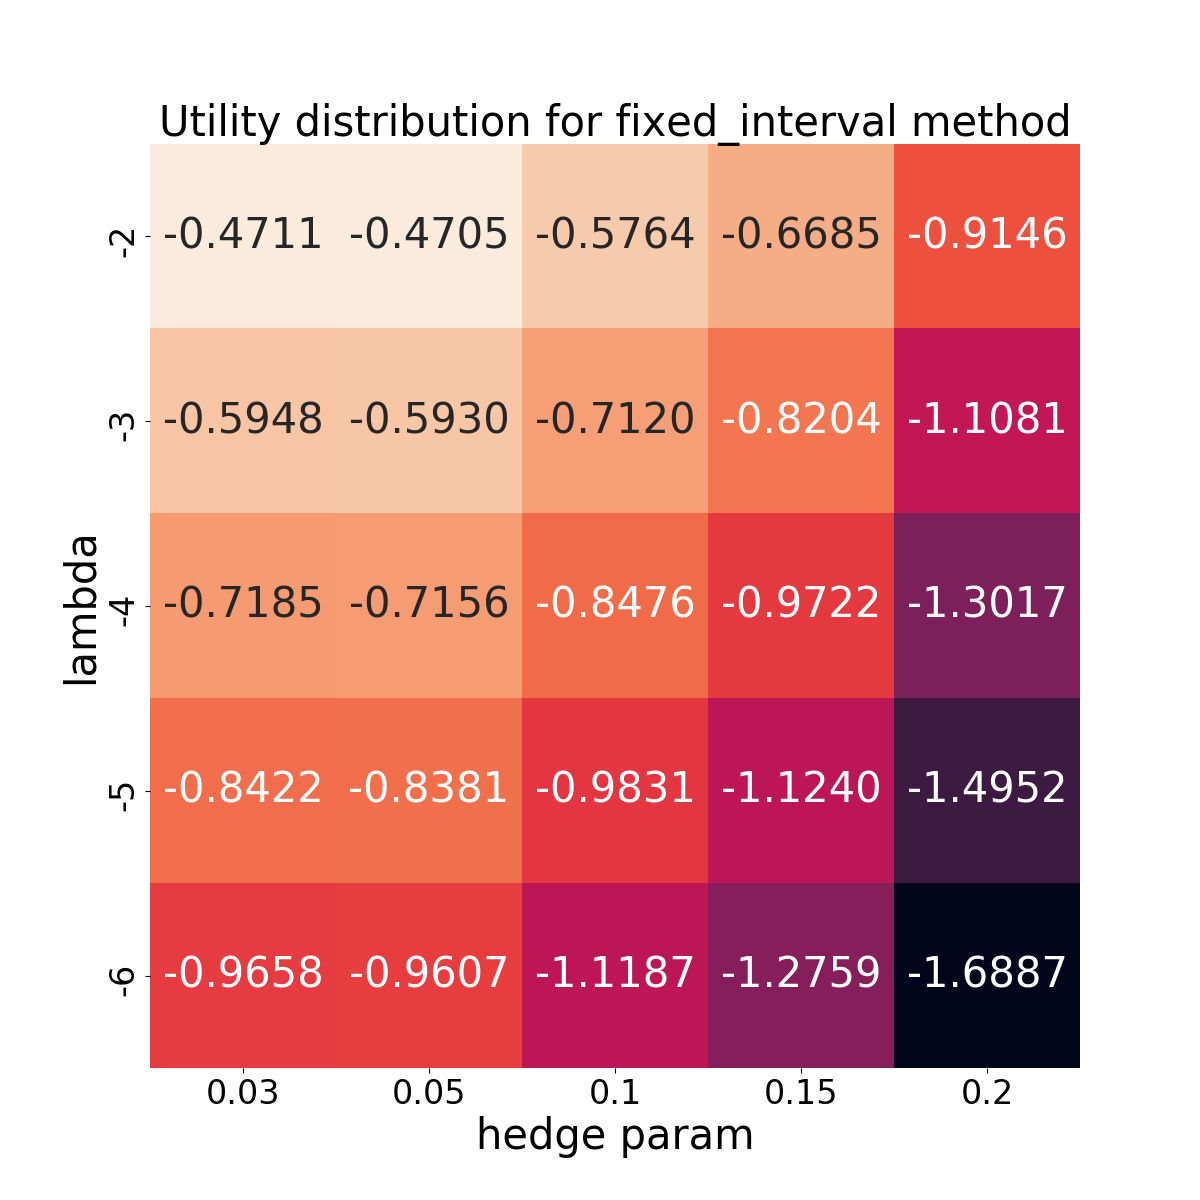
\includegraphics[width=7.5cm]{analysis/hedge_utility_real_fixed_interval_his_vol.png}}
    \caption[这里将出现在插图索引中]
    {均值-方差对冲得分}
  \label{fig:hedge_utility_real}
\end{figure}

两个策略的得分如图\ref{fig:hedge_utility_real}所示。从该图中可以看出,无论是固定时点对冲策略还是固定Delta区间对冲策略,在固定$\lambda$值时,对冲得分大致和对冲参数呈负相关关系。这一结论与模拟研究的结果类似,但是对于固定Delta区间策略,Delta阈值为0.05的结果要好于Delta阈值为0.03的结果。因此,在给定的参数范围内,对于固定时点对冲策略,场外期权交易商应当选择再平衡时间间隔为1天;对于固定Delta区间对冲策略,场外期权交易商应当选择Delta阈值为0.05。

横向对比固定时点对冲策略和固定Delta区间对冲策略,我们发现对于后四组结果,固定Delta区间对冲策略在对冲得分上的表现要明显好于固定时点对冲策略;而在第一组结果中,固定时点对冲策略较优。考虑到后四组结果中固定Delta区间对冲策略的平均再平衡次数要小于固定时点对冲策略。这说明从整体上看,固定Delta区间对冲策略还是要优于固定时点对冲策略。比较再平衡时间间隔为1天和Delta阈值为0.05的结果,我们发现,虽然固定时点对冲策略较优于固定Delta区间对冲策略,但是随着风险厌恶系数绝对值的增加,两者对冲得分的差距逐渐缩小。

基于以上实证分析,我们可以得出以下结论:场外期权交易商在对冲其动力煤看涨期权空头方向的暴露时,应当选择再平衡时间间隔为1天的固定时点动态对冲策略。

\section{进一步分析}

在以上实证分析中,动态对冲的过程我们使用了固定的波动率计算Delta。由于固定的波动率不一定能够很好地估计未来标的资产的实际波动率,因此基于此波动率的固定Delta区间动态对冲的最优策略的对冲效果要弱于固定时点动态对冲的最优策略。本节我们将探讨使用动态变化的隐含波动率对对冲效果的影响。

基于动态波动率的对冲策略具体调整如下:在每个需要计算Delta的时刻,不使用期初固定的波动率,而是利用历史波动率或EWMA波动率的算法,重新计算当天的波动率,再使用这一波动率计算Delta。虽然使用动态波动率不符合BS模型的假设,但实际上,我们可以认为这一波动率是根据某个基于动态波动率的期权定价模型的价格,代入到BS模型中计算出的隐含波动率。因此,我们是在使用这个基于动态波动率的期权定价模型。通过这一方法我们简化了计算,又可以在一定程度上反映出波动率的动态变化特点。

我们将同样使用万分之五的交易费用,分别探讨动态历史波动率和动态EWMA波动率下两个对冲策略的表现。在对冲结果的评价上,我们仍使用对冲成本率及其相关指标。在对冲成本率的计算中,我们取期初的波动率,根据BS模型计算理论价格。

\subsection{动态历史波动率}

使用动态历史波动率,两个对冲策略的对冲结果如下

\begin{table}[htbp]
  \centering
  \caption{使用动态历史波动率时固定时点动态对冲结果}
  \label{tab:fixed_time_5_his_vol_dyn}
  \begin{tabular}{cccccc}
    \toprule
    再平衡时间间隔 & 1 & 3 & 5 & 10 & 15 \\
    \midrule
    年化期望对冲成本率 & -0.14702 & -0.20816 & -0.22735 & -0.33155 & -0.54497 \\
    年化对冲成本率标准差 & 0.52481 & 0.60713 & 0.64378 & 0.66250 & 0.78371 \\
    平均再平衡次数 & 59.00000 & 19.00000 & 11.00000 & 5.00000 & 3.00000 \\
    对冲成本率偏度 & -0.91606 & -1.10890 & -1.42576 & -0.43659 & -0.55502 \\
    \bottomrule
  \end{tabular}
\end{table}

\begin{table}[htbp]
  \centering
  \caption{使用动态历史波动率时固定Delta区间动态对冲结果}
  \label{tab:fixed_interval_5_his_vol_dyn}
  \begin{tabular}{cccccc}
    \toprule
    Delta阈值 & 0.03 & 0.05 & 0.1 & 0.15 & 0.2 \\
    \midrule
    年化期望对冲成本率 & -0.15429 & -0.14672 & -0.21092 & -0.32187 & -0.44937 \\
    年化对冲成本率标准差 & 0.52015 & 0.51419 & 0.53379 & 0.58119 & 0.64752 \\
    平均再平衡次数 & 23.02341 & 15.82567 & 7.32446 & 4.28733 & 2.94754 \\
    对冲成本率偏度 & -0.87896 & -0.83628 & -0.67452 & -0.61542 & -0.42565 \\
    \bottomrule
  \end{tabular}
\end{table}

\begin{figure}[htb]
  \centering
  \subcaptionbox{固定时点动态对冲}[12cm]
    {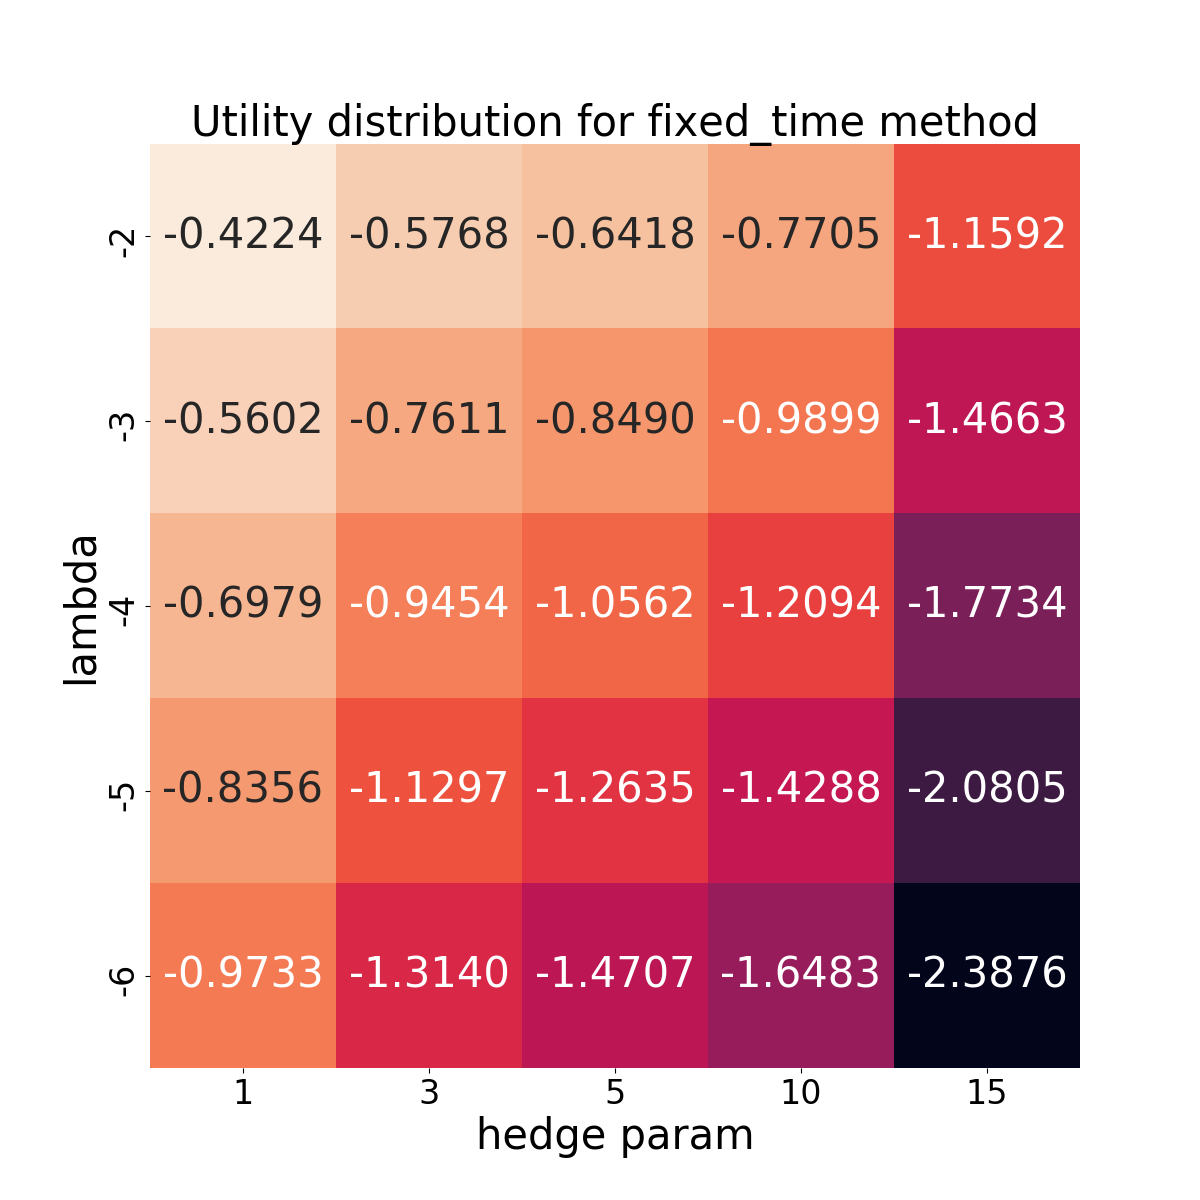
\includegraphics[width=7.5cm]{analysis/hedge_utility_real_fixed_time_his_vol_dyn.png}}
  \hspace{0.5cm}
  \subcaptionbox{固定Delta区间动态对冲}[12cm]
    {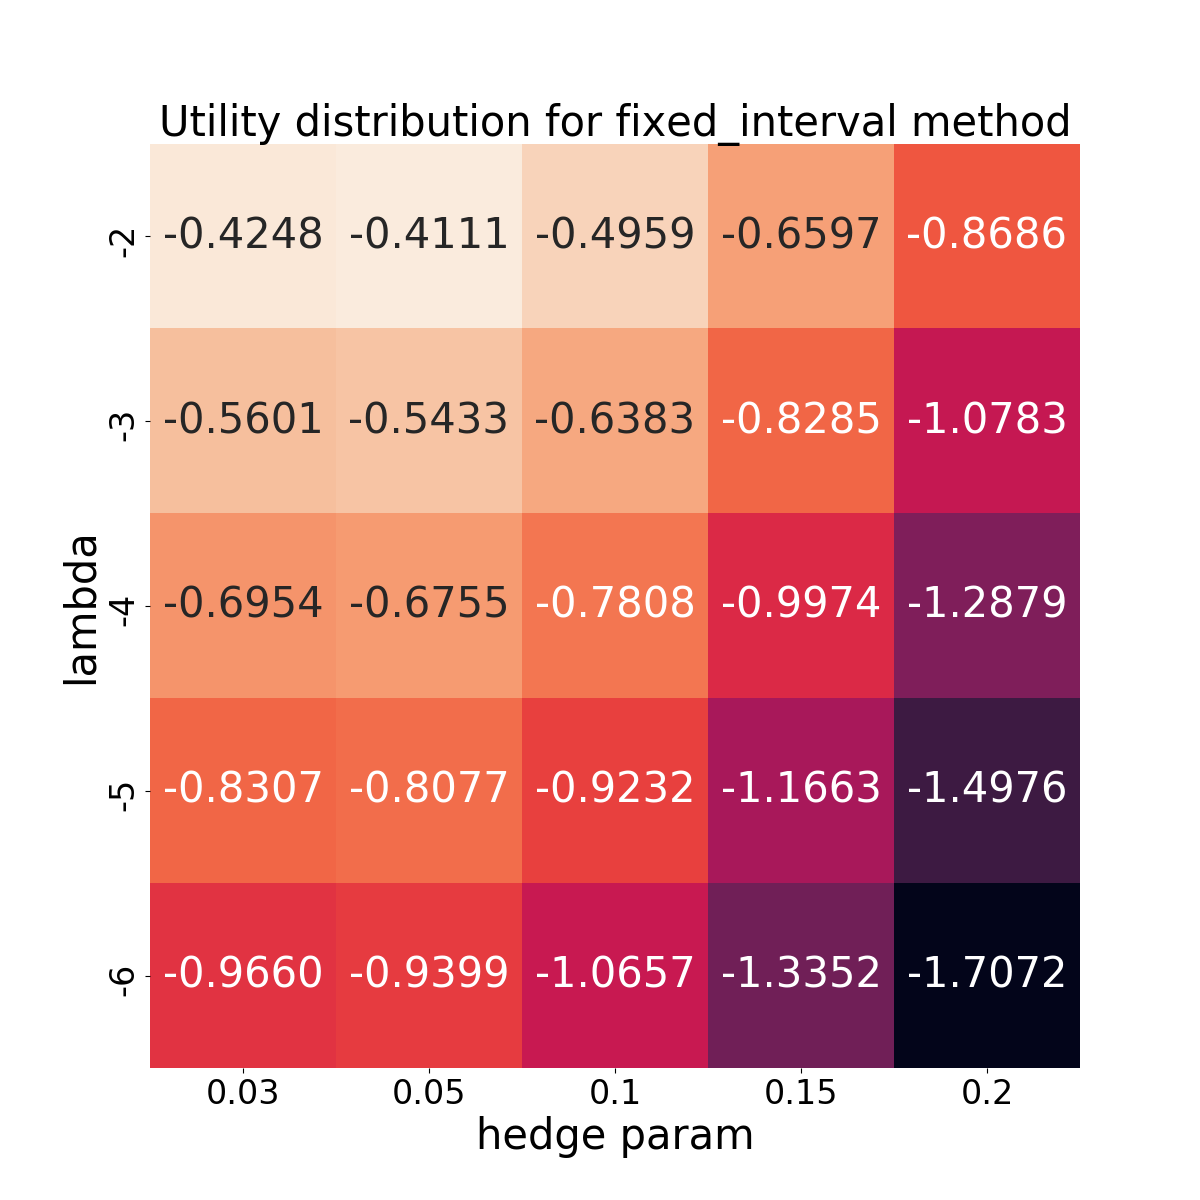
\includegraphics[width=7.5cm]{analysis/hedge_utility_real_fixed_interval_his_vol_dyn.png}}
    \caption[这里将出现在插图索引中]
    {均值-方差对冲得分}
  \label{fig:hedge_utility_real_his_dyn}
\end{figure}

根据表\ref{tab:fixed_time_5_his_vol_dyn}和表\ref{tab:fixed_interval_5_his_vol_dyn},我们发现,相对于使用固定的历史波动率,动态历史波动率对对冲效果的提升非常明显。在略微提高年化对冲成本率标准差的情况下,年化期望对冲成本率大幅下降。这说明动态历史波动率可以更好地估计动力煤指数收益率的实际波动率,从而减少对冲成本。但是,波动率本身的波动也增加了动态对冲的不确定性,从而增加对冲成本的波动率

图\ref{fig:hedge_utility_real_his_dyn}展示了动态历史波动率下,两个策略的对冲得分情况。与第\ref{utility_real}节的情况类似,再平衡时间间隔为1天和Delta阈值为0.05都分别是对应策略的最优参数。基于最优参数,横向比较两个策略的表现,我们发现在各个风险厌恶系数下,固定Delta区间动态对冲策略的表现要好于固定时点动态对冲策略的表现。这一结果第\ref{utility_real}节的情况正好相反,这也说明了动态历史波动率可以更好地反映动力煤指数收益率的波动特点。由于可以更好地估计未来波动率,因此Delta的计算也更为准确,从而使得固定Delta区间中Delta阈值可以更好地表示组合面临的一阶市场风险,实现更优的对冲效果。再纵向比较固定历史波动率和动态历史波动率的结果。我们发现,从整体上看,动态历史波动率的对冲效果更好,这也和我们上文的分析相符合。然而,当风险厌恶系数绝对值较高时,我们发现动态历史波动率下固定时点对冲策略的效果不如固定历史波动率下该策略的效果,这说明此时动态历史波动率带来的对冲波动率增加占据了主导作用。

从以上分析中,我们可以得出以下结论:使用动态历史波动率的对冲效果要优于使用固定历史波动率。在使用动态历史波动率时,Delta阈值为0.05的固定Delta区间动态对冲策略为最优对冲策略。

\subsection{动态EWMA波动率}

使用动态EWMA波动率,两个对冲策略的对冲结果如下

\begin{table}[htbp]
  \centering
  \caption{使用动态EWMA波动率时固定时点动态对冲结果}
  \label{tab:fixed_time_5_ewma_vol_dyn}
  \begin{tabular}{cccccc}
    \toprule
    再平衡时间间隔 & 1 & 3 & 5 & 10 & 15 \\
    \midrule
    年化期望对冲成本率 & -0.13483 & -0.19947 & -0.23231 & -0.35812 & -0.59882 \\
    年化对冲成本率标准差 & 0.51668 & 0.61077 & 0.65618 & 0.69238 & 0.84671 \\
    平均再平衡次数 & 59.00000 & 19.00000 & 11.00000 & 5.00000 & 3.00000 \\
    对冲成本率偏度 & -0.88096 & -1.06581 & -1.36836 & -0.58622 & -0.87452 \\
    \bottomrule
  \end{tabular}
\end{table}

\begin{table}[htbp]
  \centering
  \caption{使用动态EWMA波动率时固定Delta区间动态对冲结果}
  \label{tab:fixed_interval_5_ewma_vol_dyn}
  \begin{tabular}{cccccc}
    \toprule
    Delta阈值 & 0.03 & 0.05 & 0.1 & 0.15 & 0.2 \\
    \midrule
    年化期望对冲成本率 & -0.14822 & -0.14545 & -0.23205 & -0.31142 & -0.47579 \\
    年化对冲成本率标准差 & 0.51227 & 0.51094 & 0.56468 & 0.60591 & 0.67989 \\
    平均再平衡次数 & 24.33656 & 16.46328 & 7.65375 & 4.43745 & 3.02421 \\
    对冲成本率偏度 & -0.83515 & -0.79979 & -0.67757 & -0.64827 & -0.67477 \\
    \bottomrule
  \end{tabular}
\end{table}

\begin{figure}[htb]
  \centering
  \subcaptionbox{固定时点动态对冲}[12cm]
    {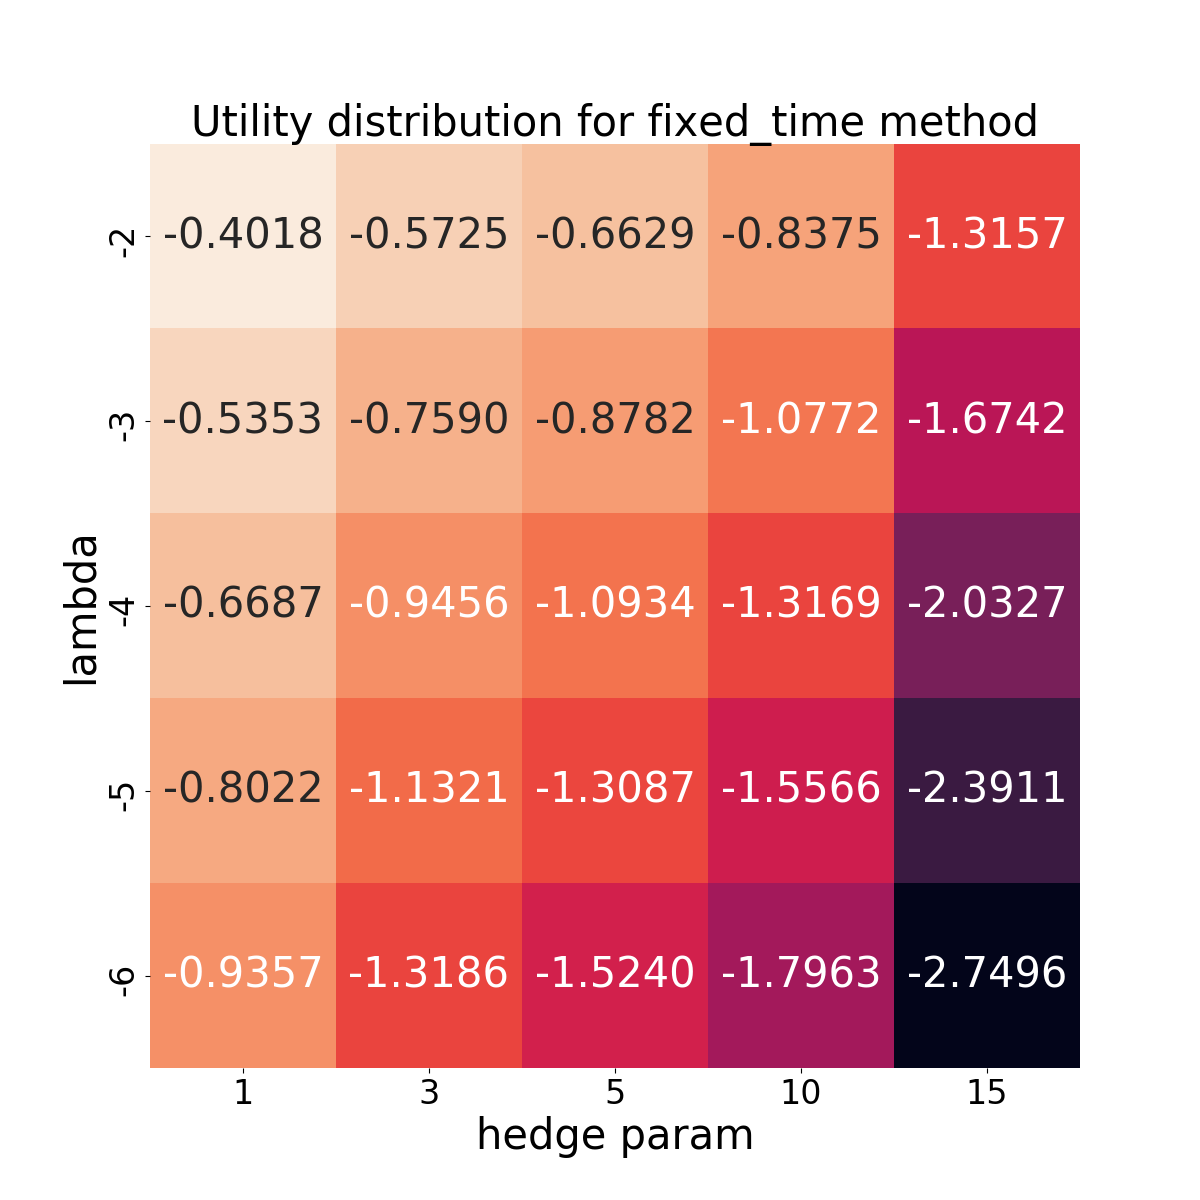
\includegraphics[width=7.5cm]{analysis/hedge_utility_real_fixed_time_ewma_vol_dyn.png}}
  \hspace{0.5cm}
  \subcaptionbox{固定Delta区间动态对冲}[12cm]
    {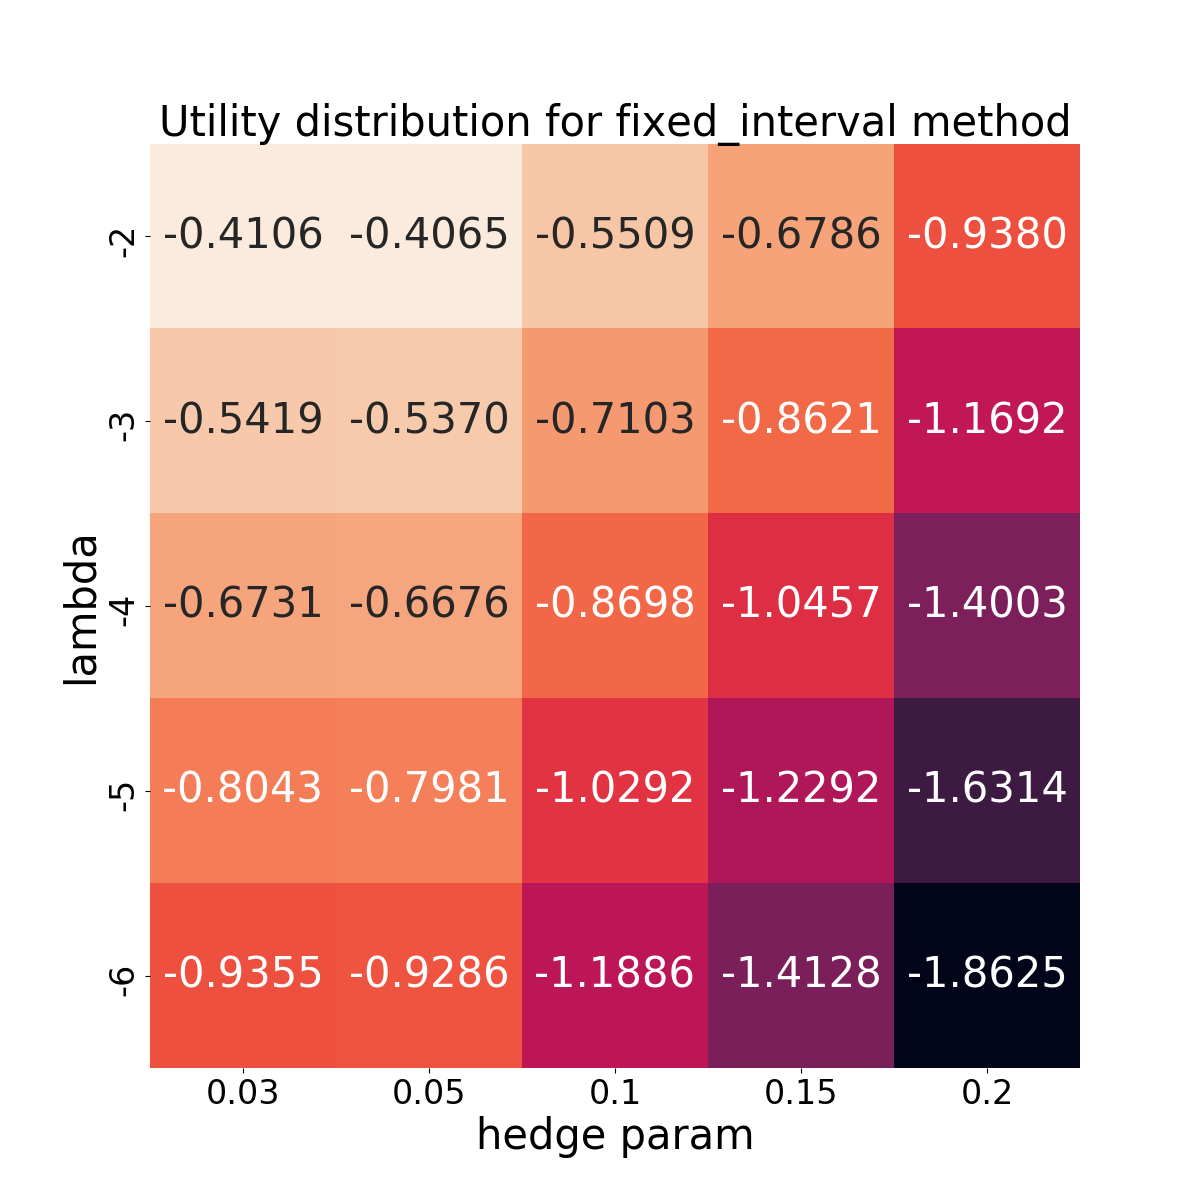
\includegraphics[width=7.5cm]{analysis/hedge_utility_real_fixed_interval_ewma_vol_dyn.png}}
    \caption[这里将出现在插图索引中]
    {均值-方差对冲得分}
  \label{fig:hedge_utility_real_ewma_dyn}
\end{figure}

与上一小节的结论类似,我们发现相对于固定EWMA波动率,动态EWMA波动率下两个策略的对冲效果均有较大提升。同时再平衡时间间隔为1天和Delta阈值为0.05夜分别是两个策略对应的最优参数。基于最优参数,横向比较两个策略的表现,我们发现当风险厌恶程度较低时,固定时点对冲策略得分较高;当风险厌恶程度较高时,固定Delta区间对冲策略更优。这说明波动率估计的准确性的提升也可以很大程度上提升固定时点对冲策略的效果。我们发现再平衡时间间隔为1天时,固定时点对冲策略的年化期望对冲成本率降到13.483\%。由于可以更精确地估计波动率,该策略可以每天根据最新的波动率计算Delta,从而实现对一阶市场风险最好的管理。当然,频繁地调整模型中的波动率也会使得对冲波动升高,从而使得在风险厌恶程度较高时,固定Delta区间对冲策略更优。

最后,根据图\ref{fig:hedge_utility_real_his_dyn}和\ref{fig:hedge_utility_real_ewma_dyn},我们比较动态历史波动率和动态EWMA波动率的结果。基于各个风险厌恶程度下选取的最优策略,我们发现动态EWMA波动率下的对冲得分均高于动态历史波动率。这与固定波动率时的结果正好相反。考虑到历史波动率的均值要高于动态EWMA波动率,这说明在动态对冲任务中,EWMA波动率对未来实际波动率的预测能力要更强,因此可以获得更好的对冲效果。

从以上分析中,我们可以得出以下结论:使用动态EWMA波动率的对冲效果不仅优于固定EWMA波动率,同时也优于动态历史波动率。在使用动态EWMA波动率时,若风险厌恶程度较低,再平衡间隔为1天的固定时点对冲策略更优,若风险厌恶程度较高,则应当选择Delta阈值为0.05的固定Delta区间对冲策略。

\section{本章小结}

本章使用动力煤指数的实际数据,对动态对冲进行了实证分析,并将结果与模拟研究的结果进行了比较。我们主要使用了历史波动率和EWMA两种波动率分别进行了实证分析。我们发现,在实际对冲操作中,与模拟研究不同,对冲不精确带来的损失远大于对冲频繁带来的额外交易成本,这说明我们应当采用对冲频率更高的动态对冲策略。这与动力煤指数收益率的分布特点有关,也取决于波动率预测的准确性。当不能够准确预测标的未来的波动率时,使用更高的对冲频率可以获得更好的对冲效果。当然,也可以通过在定价时加入波动率溢价来提高对冲效果。基于这一分析,我们得出了在实际数据上,再平衡时间间隔为1天的固定时点动态对冲策略为最优对冲策略的结论。之后,我们使用动态波动率代替固定波动率,对基于实际数据的动态对冲进行了进一步的分析。我们发现,使用动态波动率的效果明显好于固定波动率的效果,并且动态EWMA波动率更适用于动态对冲任务中未来实际波动率的预测。

%# -*- coding: utf-8-unix -*-
%%==================================================
%% chapter01.tex for SJTU Master Thesis
%%==================================================

%\bibliographystyle{sjtu2}%[此处用于每章都生产参考文献]
\chapter{总结与展望}
\label{chap:summary}

\section{结论总结}

在本文中,我们首先分析了动态对冲的理论基础以及动态对冲策略效果的影响因素。之后我们使用模拟研究和实证分析两种方法,分别基于固定时点动态对冲策略和固定Delta区间动态对冲策略,对无交易费用和有交易费用时的非连续动态对冲进行了分析和评价,并尝试探讨影响动态对冲效果的因素和比较分析模拟结果与实证结果的异同,以得出对场外期权交易商实际动态对冲操作的启示。

在模拟研究中,我们发现再平衡次数的提高在有效地降低对冲成本的波动的同时,也会由于交易费用的引入而提高期望对冲成本。基于我们推导的均值-方差对冲得分评判标准,降低对冲成本的波动对最终得分的正面影响要超过期望对冲成本增加带来的负面影响。在此基础上,我们得出了固定Delta区间对冲策略要优于固定时点对冲策略的结论,并且在给定的参数范围内,Delta阈值的选择取决于对冲者的风险厌恶程度。

在实证分析中,我们使用了动力煤指数的数据,进行了动态对冲策略的滚动回测。我们发现,实证分析和模拟研究结果上的差异主要在两方面:1)实证结果中无论是期望对冲成本还是对冲成本波动均高于模拟结果。这一差异既有实证研究中数据不足,带来的收敛性不佳的原因,更主要是因为实证分析中难以对未来波动率有准确的估计从而导致Delta计算的不准确,由此带来更高的对冲成本和对冲成本波动。2)实证结果中再平衡次数越高,期望对冲成本反而越高。这说明在实际操作中,对冲不精确对对冲成本的影响要大于一定范围内交易费用增加对对冲成本的影响。因此,虽然整体上看固定Delta区间对冲策略要优于固定时点对冲策略,这与模拟研究的结果相同并且可以同样地得到解释,但是在最优策略的选择上,我们选择了再平衡时间间隔为1天的固定时点对冲策略。

综上所述,从理论和模拟分析上,在综合考虑交易费用之后固定Delta区间动态对冲策略要优于固定时点动态对冲策略。但是,在实际市场操作中,对冲效果受交易费用影响较小,主要取决于对冲的精确程度。由于固定Delta区间动态对冲需要人为估计标的资产的未来实际波动率,这一估计的准确性将直接影响到对冲效果。因此,在不能够准确估计标的资产未来波动率时,使用再平衡频率较高的固定时点对冲策略更优。对于对冲中出现的对冲成本,场外期权交易商在定价时应当合理制定波动率溢价,这不仅可以降低最终的期望对冲成本,还可以降低对冲成本的波动。

% %# -*- coding: utf-8-unix -*-
%%==================================================
%% chapter02.tex for SJTU Master Thesis
%% based on CASthesis
%% modified by wei.jianwen@gmail.com
%% Encoding: UTF-8
%%==================================================

\chapter{{\LaTeX} 排版例子}
\label{chap:example}

\section{列表环境}
\label{sec:list}

\subsection{无序列表}
\label{sec:unorderlist}

以下是一个无序列表的例子,列表的每个条目单独分段。

\begin{itemize}
  \item 这是一个无序列表。
  \item 这是一个无序列表。
  \item 这是一个无序列表。
\end{itemize}

使用\verb+itemize*+环境可以创建行内无序列表。
\begin{itemize*}
  \item 这是一个无序列表。
  \item 这是一个无序列表。
  \item 这是一个无序列表。
\end{itemize*}
行内无序列表条目不单独分段,所有内容直接插入在原文的段落中。

\subsection{有序列表}
\label{sec:orderlist}

使用环境\verb+enumerate+和\verb+enumerate*+创建有序列表,
使用方法无序列表类似。

\begin{enumerate}
  \item 这是一个有序列表。
  \item 这是一个有序列表。
  \item 这是一个有序列表。
\end{enumerate}

使用\verb+enumerate*+环境可以创建行内有序列表。
\begin{enumerate*}
  \item 这是一个默认有序列表。
  \item 这是一个默认有序列表。
  \item 这是一个默认有序列表。
\end{enumerate*}
行内有序列表条目不单独分段,所有内容直接插入在原文的段落中。

\subsection{描述型列表}

使用环境\verb+description+可创建带有主题词的列表,条目语法是\verb+\item[主题] 内容+。
\begin{description}
    \item[主题一] 详细内容
    \item[主题二] 详细内容
    \item[主题三] 详细内容 \ldots
\end{description}

\subsection{自定义列表样式}

可以使用\verb+label+参数控制列表的样式,
详细可以参考WikiBooks\footnote{\url{https://en.wikibooks.org/wiki/LaTeX/List_Structures\#Customizing_lists}}。
比如一个自定义样式的行内有序列表
\begin{enumerate*}[label=\itshape\alph*)\upshape]
  \item 这是一个自定义样式有序列表。
  \item 这是一个自定义样式有序列表。
  \item 这是一个自定义样式有序列表。
\end{enumerate*}

\section{数学排版}
\label{sec:matheq}

\subsection{公式排版}
\label{sec:eqformat}

这里有举一个长公式排版的例子,来自\href{http://www.tex.ac.uk/tex-archive/info/math/voss/mathmode/Mathmode.pdf}{《Math mode》}:

\begin {multline}
  \frac {1}{2}\Delta (f_{ij}f^{ij})=
  2\left (\sum _{i<j}\chi _{ij}(\sigma _{i}-
    \sigma _{j}) ^{2}+ f^{ij}\nabla _{j}\nabla _{i}(\Delta f)+\right .\\
  \left .+\nabla _{k}f_{ij}\nabla ^{k}f^{ij}+
    f^{ij}f^{k}\left [2\nabla _{i}R_{jk}-
      \nabla _{k}R_{ij}\right ]\vphantom {\sum _{i<j}}\right )
\end{multline}

\subsection{SI单位}

使用\verb+siunitx+宏包可以方便地输入SI单位制单位,例如\verb+\SI{5}{\um}+可以得到\SI{5}{\um}。

\subsubsection{一个四级标题}
\label{sec:depth4}

这是全文唯一的一个四级标题。在这部分中将演示了mathtools宏包中可伸长符号(箭头、等号的例子)的例子。

\begin{displaymath}
    A \xleftarrow[n=0]{} B \xrightarrow[LongLongLongLong]{n>0} C
\end{displaymath}

\begin{eqnarray}
  f(x) & \xleftrightarrow[]{A=B}  & B \\
  & \xleftharpoondown[below]{above} & B \nonumber \\
  & \xLeftrightarrow[below]{above} & B
\end{eqnarray}

又如:

\begin{align}
  \label{eq:none}
  & I(X_3;X_4)-I(X_3;X_4\mid{}X_1)-I(X_3;X_4\mid{}X_2) \nonumber \\
  = & [I(X_3;X_4)-I(X_3;X_4\mid{}X_1)]-I(X_3;X_4\mid{}\tilde{X}_2) \\
  = & I(X_1;X_3;X_4)-I(X_3;X_4\mid{}\tilde{X}_2)
\end{align}

\subsection{定理环境}

模板中定义了丰富的定理环境
algo(算法),thm(定理),lem(引理),prop(命题),cor(推论),defn(定义),conj(猜想),exmp(例),rem(注),case(情形),
bthm(断言定理),blem(断言引理),bprop(断言命题),bcor(断言推论)。
amsmath还提供了一个proof(证明)的环境。
这里举一个“定理”和“证明”的例子。
\begin{thm}[留数定理]
\label{thm:res}
  假设$U$是复平面上的一个单连通开子集,$a_1,\ldots,a_n$是复平面上有限个点,$f$是定义在$U\backslash \{a_1,\ldots,a_n\}$上的全纯函数,
  如果$\gamma$是一条把$a_1,\ldots,a_n$包围起来的可求长曲线,但不经过任何一个$a_k$,并且其起点与终点重合,那么:

  \begin{equation}
    \label{eq:res}
    \ointop_{\gamma}f(z)\,\mathrm{d}z = 2\uppi\mathbf{i}\sum^n_{k=1}\mathrm{I}(\gamma,a_k)\mathrm{Res}(f,a_k)
  \end{equation}

  如果$\gamma$是若尔当曲线,那么$\mathrm{I}(\gamma, a_k)=1$,因此:

  \begin{equation}
    \label{eq:resthm}
    \ointop_{\gamma}f(z)\,\mathrm{d}z = 2\uppi\mathbf{i}\sum^n_{k=1}\mathrm{Res}(f,a_k)
  \end{equation}

      % \oint_\gamma f(z)\, dz = 2\pi i \sum_{k=1}^n \mathrm{Res}(f, a_k ).

  在这里,$\mathrm{Res}(f, a_k)$表示$f$在点$a_k$的留数,$\mathrm{I}(\gamma,a_k)$表示$\gamma$关于点$a_k$的卷绕数。
  卷绕数是一个整数,它描述了曲线$\gamma$绕过点$a_k$的次数。如果$\gamma$依逆时针方向绕着$a_k$移动,卷绕数就是一个正数,
  如果$\gamma$根本不绕过$a_k$,卷绕数就是零。

  定理\ref{thm:res}的证明。

  \begin{proof}
    首先,由……

    其次,……

    所以……
  \end{proof}
\end{thm}

上面的公式例子中,有一些细节希望大家注意。微分号d应该使用“直立体”也就是用mathrm包围起来。
并且,微分号和被积函数之间应该有一段小间隔,可以插入\verb+\,+得到。
斜体的$d$通常只作为一般变量。
i,j作为虚数单位时,也应该使用“直立体”为了明显,还加上了粗体,例如\verb+\mathbf{i}+。斜体$i,j$通常用作表示“序号”。
其他字母在表示常量时,也推荐使用“直立体”譬如,圆周率$\uppi$(需要upgreek宏包),自然对数的底$\mathrm{e}$。
不过,我个人觉得斜体的$e$和$\pi$很潇洒,在不至于引起混淆的情况下,我也用这两个字母的斜体表示对应的常量。


\section{向文档中插入图像}
\label{sec:insertimage}

\subsection{支持的图片格式}
\label{sec:imageformat}

\XeTeX 可以很方便地插入PDF、PNG、JPG格式的图片。

插入PNG/JPG的例子如\ref{fig:SRR}所示。
这两个水平并列放置的图共享一个“图标题”(table caption),没有各自的小标题。

\begin{figure}[!htp]
  \centering
  
\includegraphics[width=4cm]{example/sjtulogo.png}
  \hspace{1cm}
  
\includegraphics[width=4cm]{example/sjtulogo.jpg}
  \bicaption[这里将出现在插图索引中]
    {中文题图}
    {English caption}
  \label{fig:SRR}
\end{figure}

这里还有插入EPS图像和PDF图像的例子,如图\ref{fig:epspdf:a}和图\ref{fig:epspdf:b}。这里将EPS和PDF图片作为子图插入,每个子图有自己的小标题。子图标题使用subcaption宏包添加。

\begin{figure}[!htp]
  \centering
  \subcaptionbox{EPS 图像\label{fig:epspdf:a}}[3cm] %标题的长度,超过则会换行,如下一个小图。
    {
\includegraphics[height=2.5cm]{example/sjtulogo.eps}}
  \hspace{4em}
  \subcaptionbox{PDF 图像,注意这个图略矮些。如果标题很长的话,它会自动换行\label{fig:epspdf:b}}
    {
\includegraphics[height=2cm]{sjtulogo.pdf}}
  \bicaption{插入eps和pdf的例子(使用 subcaptionbox 方式)}{An EPS and PDF demo with subcaptionbox}
  \label{fig:pdfeps-subcaptionbox}
\end{figure}

\begin{figure}[!htp]
  \centering
  \begin{subfigure}{2.5cm}
    \centering
    
\includegraphics[height=2.5cm]{example/sjtulogo.eps}
    \caption{EPS 图像}
  \end{subfigure}
  \hspace{4em}
  \begin{subfigure}{0.4\textwidth}
    \centering
    
\includegraphics[height=2cm]{sjtulogo.pdf}
    \caption{PDF 图像,注意这个图略矮些。subfigure中同一行的子图在顶端对齐。}
  \end{subfigure}
  \bicaption{插入eps和pdf的例子(使用 subfigure 方式)}{An EPS and PDF demo with subfigure}
  \label{fig:pdfeps-subfigure}
\end{figure}

更多关于 \LaTeX 插图的例子可以参考\href{http://www.cs.duke.edu/junhu/Graphics3.pdf}{《\LaTeX 插图指南》}。

\subsection{长标题的换行}
\label{sec:longcaption}

图\ref{fig:longcaptionbad}和图\ref{fig:longcaptiongood}都有比较长图标题,通过对比发现,图\ref{fig:longcaptiongood}的换行效果更好一些。
其中使用了minipage环境来限制整个浮动体的宽度。

\begin{figure}[!htp]
  \centering
  
\includegraphics[width=4cm]{sjtubadge.pdf}
  \bicaption[这里将出现在插图索引]
    {上海交通大学是我国历史最悠久的高等学府之一,是教育部直属、教育部与上海市共建的全国重点大学.}
    {Where there is a will, there is a way.}
 \label{fig:longcaptionbad}
\end{figure}

\begin{figure}[!htbp]
  \centering
  \begin{minipage}[b]{0.6\textwidth}
    \centering
    
\includegraphics[width=4cm]{sjtubadge.pdf}
    \bicaption[出现在插图索引中]
      {上海交通大学是我国历史最悠久的高等学府之一,是教育部直属、教育部与上海市共建的全国重点大学.}
      {Where there is a will, there is a way.}
    \label{fig:longcaptiongood}
  \end{minipage}
\end{figure}

\subsection{绘制流程图}

图\ref{fig:flow_chart}是一张流程图示意。使用tikz环境,搭配四种预定义节点(\verb+startstop+、\verb+process+、\verb+decision+和\verb+io+),可以容易地绘制出流程图。
\begin{figure}[!htp]
    \centering
    \resizebox{6cm}{!}{\begin{tikzpicture}[node distance=2cm]
    \node (pic) [startstop] {待测图片};
    \node (bg) [io, below of=pic] {读取背景};
    \node (pair) [process, below of=bg] {匹配特征点对};
    \node (threshold) [decision, below of=pair, yshift=-0.5cm] {多于阈值};
    \node (clear) [decision, right of=threshold, xshift=3cm] {清晰?};
    \node (capture) [process, right of=pair, xshift=3cm, yshift=0.5cm] {重采};
    \node (matrix_p) [process, below of=threshold, yshift=-0.8cm] {透视变换矩阵};
    \node (matrix_a) [process, right of=matrix_p, xshift=3cm] {仿射变换矩阵};
    \node (reg) [process, below of=matrix_p] {图像修正};
    \node (return) [startstop, below of=reg] {配准结果};
     
    %连接具体形状
    \draw [arrow](pic) -- (bg);
    \draw [arrow](bg) -- (pair);
    \draw [arrow](pair) -- (threshold);

    \draw [arrow](threshold) -- node[anchor=south] {否} (clear);

    \draw [arrow](clear) -- node[anchor=west] {否} (capture);
    \draw [arrow](capture) |- (pic);
    \draw [arrow](clear) -- node[anchor=west] {是} (matrix_a);
    \draw [arrow](matrix_a) |- (reg);

    \draw [arrow](threshold) -- node[anchor=east] {是} (matrix_p);
    \draw [arrow](matrix_p) -- (reg);
    \draw [arrow](reg) -- (return);
\end{tikzpicture}
}
    \bicaption{绘制流程图效果}{Flow chart}
    \label{fig:flow_chart}
\end{figure}

\clearpage

\section{表格}
\label{sec:tab}

这一节给出的是一些表格的例子,如表\ref{tab:firstone}所示。

\begin{table}[!hpb]
  \centering
  \caption{一个颇为标准的三线表格}
  \label{tab:firstone}
  \begin{tabular}{@{}llr@{}} \toprule
    \multicolumn{2}{c}{Item} \\ \cmidrule(r){1-2}
    Animal & Description & Price (\$)\\ \midrule
    Gnat & per gram & 13.65 \\
    & each & 0.01 \\
    Gnu & stuffed & 92.50 \\
    Emu & stuffed & 33.33 \\
    Armadillo & frozen & 8.99 \\ \bottomrule
  \end{tabular}
\end{table}
\footnotetext[1]{这个例子来自\href{http://www.ctan.org/tex-archive/macros/latex/contrib/booktabs/booktabs.pdf}{《Publication quality tables in LATEX》}(booktabs宏包的文档)。这也是一个在表格中使用脚注的例子,请留意与threeparttable实现的效果有何不同。}

下面一个是一个更复杂的表格,用threeparttable实现带有脚注的表格,如表\ref{tab:footnote}。

\begin{table}[!htpb]
  \bicaption[出现在表目录的标题]
    {一个带有脚注的表格的例子}
    {A Table with footnotes}
  \label{tab:footnote}
  \centering
  \begin{threeparttable}[b]
     \begin{tabular}{ccd{4}cccc}
      \toprule
      \multirow{2}{6mm}{total}&\multicolumn{2}{c}{20\tnote{1}} & \multicolumn{2}{c}{40} &  \multicolumn{2}{c}{60}\\
      \cmidrule(lr){2-3}\cmidrule(lr){4-5}\cmidrule(lr){6-7}
      &www & \multicolumn{1}{c}{k} & www & k & www & k \\ % 使用说明符 d 的列会自动进入数学模式,使用 \multicolumn 对文字表头做特殊处理
      \midrule
      &$\underset{(2.12)}{4.22}$ & 120.0140\tnote{2} & 333.15 & 0.0411 & 444.99 & 0.1387 \\
      &168.6123 & 10.86 & 255.37 & 0.0353 & 376.14 & 0.1058 \\
      &6.761    & 0.007 & 235.37 & 0.0267 & 348.66 & 0.1010 \\
      \bottomrule
    \end{tabular}
    \begin{tablenotes}
    \item [1] the first note.% or \item [a]
    \item [2] the second note.% or \item [b]
    \end{tablenotes}
  \end{threeparttable}
\end{table}

\section{参考文献管理}

 \LaTeX 具有将参考文献内容和表现形式分开管理的能力,涉及三个要素:参考文献数据库、参考文献引用格式、在正文中引用参考文献。
这样的流程需要多次编译:

\begin{enumerate}[noitemsep,topsep=0pt,parsep=0pt,partopsep=0pt]
	\item 用户将论文中需要引用的参考文献条目,录入纯文本数据库文件(bib文件)。
	\item 调用xelatex对论文模板做第一次编译,扫描文中引用的参考文献,生成参考文献入口文件(aux)文件。
	\item 调用bibtex,以参考文献格式和入口文件为输入,生成格式化以后的参考文献条目文件(bib)。
	\item 再次调用xelatex编译模板,将格式化以后的参考文献条目插入正文。
\end{enumerate}

参考文献数据库(thesis.bib)的条目,可以从Google Scholar搜索引擎\footnote{\url{https://scholar.google.com}}、CiteSeerX搜索引擎\footnote{\url{http://citeseerx.ist.psu.edu}}中查找,文献管理软件Papers\footnote{\url{http://papersapp.com}}、Mendeley\footnote{\url{http://www.mendeley.com}}、JabRef\footnote{\url{http://jabref.sourceforge.net}}也能够输出条目信息。

下面是在Google Scholar上搜索到的一条文献信息,格式是纯文本:

\begin{lstlisting}[caption={从Google Scholar找到的参考文献条目}, label=googlescholar, escapeinside="", numbers=none]
    @phdthesis{"白2008信用风险传染模型和信用衍生品的定价",
      title={"信用风险传染模型和信用衍生品的定价"},
      author={"白云芬"},
      year={2008},
      school={"上海交通大学"}
    }
\end{lstlisting}

推荐修改后在bib文件中的内容为:

\begin{lstlisting}[caption={修改后的参考文献条目}, label=itemok, escapeinside="", numbers=none]
  @phdthesis{bai2008,
    title={"信用风险传染模型和信用衍生品的定价"},
    author={"白云芬"},
    date={2008},
    address={"上海"},
    school={"上海交通大学"}
  }
\end{lstlisting}

按照教务处的要求,参考文献外观应符合国标GBT7714的要求\footnote{\url{http://www.cces.net.cn/guild/sites/tmxb/Files/19798_2.pdf}}。
在模板中,表现形式的控制逻辑通过biblatex-gb7714-2015包实现\footnote{\url{https://www.ctan.org/pkg/biblatex-gb7714-2015}},基于{Bib\LaTeX}管理文献。在目前的多数TeX发行版中,可能都没有默认包含biblatex-gb7714-2015,需要手动安装。

正文中引用参考文献时,用\verb+\cite{key1,key2,key3...}+可以产生“上标引用的参考文献”,
如\cite{Meta_CN,chen2007act,DPMG}。
使用\verb+\parencite{key1,key2,key3...}+则可以产生水平引用的参考文献,例如\parencite{JohnD,zhubajie,IEEE-1363}。
请看下面的例子,将会穿插使用水平的和上标的参考文献:关于书的\parencite{Meta_CN,JohnD,IEEE-1363},关于期刊的\cite{chen2007act,chen2007ewi},
会议论文\parencite{DPMG,kocher99,cnproceed},
硕士学位论文\parencite{zhubajie,metamori2004},博士学位论文\cite{shaheshang,FistSystem01,bai2008},标准文件\parencite{IEEE-1363},技术报告\cite{NPB2},电子文献\parencite{xiaoyu2001, CHRISTINE1998},用户手册\parencite{RManual}。

总结一些注意事项:
\begin{itemize}
\item 参考文献只有在正文中被引用了,才会在最后的参考文献列表中出现;
\item 参考文献“数据库文件”bib是纯文本文件,请使用UTF-8编码,不要使用GBK编码;
\item 参考文献条目中默认通过date域输入时间。兼容使用year域时会产生编译warning,可忽略。
\end{itemize}

\section{用listings插入源代码}

原先ctexbook文档类和listings宏包配合使用时,代码在换页时会出现莫名其妙的错误,后来经高人指点,顺利解决了。
感兴趣的话,可以看看\href{http://bbs.ctex.org/viewthread.php?tid=53451}{这里}。
这里给使用listings宏包插入源代码的例子,这里是一段C代码。
另外,listings宏包真可谓博大精深,可以实现各种复杂、漂亮的效果,想要进一步学习的同学,可以参考
\href{http://mirror.ctan.org/macros/latex/contrib/listings/listings.pdf}{listings宏包手册}。

\begin{lstlisting}[language={C}, caption={一段C源代码}]
#include <stdio.h>
#include <unistd.h>
#include <sys/types.h>
#include <sys/wait.h>

int main() {
  pid_t pid;

  switch ((pid = fork())) {
  case -1:
    printf("fork failed\n");
    break;
  case 0:
    /* child calls exec */
    execl("/bin/ls", "ls", "-l", (char*)0);
    printf("execl failed\n");
    break;
  default:
    /* parent uses wait to suspend execution until child finishes */
    wait((int*)0);
    printf("is completed\n");
    break;
  }

  return 0;
}
\end{lstlisting}

\section{用algorithm和algorithmicx宏包插入算法描述}

algorithmicx 比 algorithmic 增加了一些命令。
示例如算法\ref{algo:sum_100}和算法\ref{algo:merge_sort},
后者的代码来自\href{http://hustsxh.is-programmer.com/posts/38801.html}{xhSong的博客}。
algorithmicx的详细使用方法见\href{http://mirror.hust.edu.cn/CTAN/macros/latex/contrib/algorithmicx/algorithmicx.pdf}{官方README}。
使用算法宏包时,算法出现的位置很多时候不按照tex文件里的书写顺序,
需要强制定位时可以使用\verb+\begin{algorithm}[H]+
\footnote{http://tex.stackexchange.com/questions/165021/fixing-the-location-of-the-appearance-in-algorithmicx-environment}

这是写在算法\ref{algo:sum_100}前面的一段话,在生成的文件里它会出现在算法\ref{algo:sum_100}前面。

\begin{algorithm}
% \begin{algorithm}[H] % 强制定位
\caption{求100以内的整数和}
\label{algo:sum_100}
\begin{algorithmic}[1] %每行显示行号
\Ensure 100以内的整数和 % 输出
\State $sum \gets 0$
\For{$i = 0 \to 100$}
    \State $sum \gets sum + i$
  \EndFor
\end{algorithmic}
\end{algorithm}

这是写在两个算法中间的一段话,当算法\ref{algo:sum_100}不使用\verb+\begin{algorithm}[H]+时它也会出现在算法\ref{algo:sum_100}前面。

对于很长的算法,单一的算法块\verb+\begin{algorithm}...\end{algorithm}+是不能自动跨页的
\footnote{http://tex.stackexchange.com/questions/70733/latex-algorithm-not-display-under-correct-section},
会出现的情况有:

\begin{itemize}
  \item 该页放不下当前的算法,留下大片空白,算法在下一页显示
  \item 单一页面放不下当前的算法,显示时超过页码的位置直到超出整个页面范围
\end{itemize}

解决方法有:

\begin{itemize}
  \item (推荐)使用\verb+algstore{algname}+和\verb+algrestore{algname}+来讲算法分为两个部分\footnote{http://tex.stackexchange.com/questions/29816/algorithm-over-2-pages},如算法\ref{algo:merge_sort}。
  \item 人工拆分算法为多个小的部分。
\end{itemize}

\begin{algorithm}
% \begin{algorithm}[H] % 强制定位
\caption{用归并排序求逆序数}
\label{algo:merge_sort}
\begin{algorithmic}[1] %每行显示行号
\Require $Array$数组,$n$数组大小 % 输入
\Ensure 逆序数 % 输出
\Function {MergerSort}{$Array, left, right$}
  \State $result \gets 0$
  \If {$left < right$}
    \State $middle \gets (left + right) / 2$
    \State $result \gets result +$ \Call{MergerSort}{$Array, left, middle$}
    \State $result \gets result +$ \Call{MergerSort}{$Array, middle, right$}
    \State $result \gets result +$ \Call{Merger}{$Array,left,middle,right$}
  \EndIf
  \State \Return{$result$}
\EndFunction
\State %空一行
\Function{Merger}{$Array, left, middle, right$}
  \State $i\gets left$
  \State $j\gets middle$
  \State $k\gets 0$
  \State $result \gets 0$
  \While{$i<middle$ \textbf{and} $j<right$}
    \If{$Array[i]<Array[j]$}
      \State $B[k++]\gets Array[i++]$
    \Else
      \State $B[k++] \gets Array[j++]$
      \State $result \gets result + (middle - i)$
    \EndIf
  \EndWhile
  \algstore{MergeSort}
\end{algorithmic}
\end{algorithm}

\begin{algorithm}
\begin{algorithmic}[1]
  \algrestore{MergeSort}
  \While{$i<middle$}
    \State $B[k++] \gets Array[i++]$
  \EndWhile
  \While{$j<right$}
    \State $B[k++] \gets Array[j++]$
  \EndWhile
  \For{$i = 0 \to k-1$}
    \State $Array[left + i] \gets B[i]$
  \EndFor
  \State \Return{$result$}
\EndFunction
\end{algorithmic}
\end{algorithm}

这是写在算法\ref{algo:merge_sort}后面的一段话,
但是当算法\ref{algo:merge_sort}不使用\verb+\begin{algorithm}[H]+时它会出现在算法\ref{algo:merge_sort}
甚至算法\ref{algo:sum_100}前面。

对于算法的索引要注意\verb+\caption+和\verb+\label+的位置,
必须是先\verb+\caption+再\verb+\label+\footnote{http://tex.stackexchange.com/questions/65993/algorithm-numbering},
否则会出现\verb+\ref{algo:sum_100}+生成的编号跟对应算法上显示不一致的问题。

根据Werner的回答\footnote{http://tex.stackexchange.com/questions/53357/switch-cases-in-algorithmic}
增加了\verb+Switch+和\verb+Case+的支持,见算法\ref{algo:switch_example}。

\begin{algorithm}
\caption{Switch示例}
\label{algo:switch_example}
\begin{algorithmic}[1]
  \Switch{$s$}
    \Case{$a$}
      \Assert{0}
    \EndCase
    \Case{$b$}
      \Assert{1}
    \EndCase
    \Default
      \Assert{2}
    \EndDefault
  \EndSwitch
\end{algorithmic}
\end{algorithm}



\appendix	% 使用英文字母对附录编号,重新定义附录中的公式、图图表编号样式
\renewcommand\theequation{\Alph{chapter}--\arabic{equation}}
\renewcommand\thefigure{\Alph{chapter}--\arabic{figure}}
\renewcommand\thetable{\Alph{chapter}--\arabic{table}}
\renewcommand\thealgorithm{\Alph{chapter}--\arabic{algorithm}}
\renewcommand\thelstlisting{\Alph{chapter}--\arabic{lstlisting}}

%% 附录内容,本科学位论文可以用翻译的文献替代。
%# -*- coding: utf-8-unix -*-
\chapter{有交易费用时动态对冲结果}
\label{app:sim_fee_result}

\begin{table}[htbp]
  \centering
  \caption{交易费用为0.02\%时固定时点动态对冲结果}
  \label{tab:fixed_time_0.02}
  \begin{tabular}{cccccc}
    \toprule
    再平衡时间间隔 & 1 & 3 & 5 & 10 & 15 \\
    \midrule
    期望对冲成本 & 4.30561 & 4.28920 & 4.28376 & 4.28176 & 4.28586 \\
    对冲成本标准差 & 0.43158 & 0.73533 & 0.93654 & 1.29693 & 1.57283 \\
    相对对冲波动率 & 0.10169 & 0.17326 & 0.22067 & 0.30558 & 0.37059 \\
    平均再平衡次数 & 59.00000 & 19.00000 & 11.00000 & 5.00000 & 3.00000 \\
    对冲成本偏度 & 0.29935 & 0.34396 & 0.39725 & 0.52199 & 0.60036 \\
    \bottomrule
  \end{tabular}
\end{table}

\begin{table}[htbp]
  \centering
  \caption{交易费用为0.02\%时固定Delta区间动态对冲结果}
  \label{tab:fixed_interval_0.02}
  \begin{tabular}{cccccc}
    \toprule
    Delta阈值 & 0.03 & 0.05 & 0.1 & 0.15 & 0.2 \\
    \midrule
    期望对冲成本 & 4.30085 & 4.29790 & 4.29405 & 4.29665 & 4.29188 \\
    对冲成本标准差 & 0.44602 & 0.48299 & 0.63697 & 0.83624 & 1.01050 \\
    相对对冲波动率 & 0.10509 & 0.11380 & 0.15008 & 0.19703 & 0.23809 \\
    平均再平衡次数 & 29.40615 & 20.23458 & 9.30930 & 5.20800 & 3.36844 \\
    对冲成本偏度 & 0.25321 & 0.18972 & 0.13359 & 0.22417 & 0.19394 \\
    \bottomrule
  \end{tabular}
\end{table}

\begin{table}[htbp]
  \centering
  \caption{交易费用为0.05\%时固定时点动态对冲结果}
  \label{tab:fixed_time_0.05}
  \begin{tabular}{cccccc}
    \toprule
    再平衡时间间隔 & 1 & 3 & 5 & 10 & 15 \\
    \midrule
    期望对冲成本 & 4.39561 & 4.34789 & 4.33305 & 4.32361 & 4.32463 \\
    对冲成本标准差 & 0.43758 & 0.73584 & 0.93816 & 1.30429 & 1.57513 \\
    相对对冲波动率 & 0.10310 & 0.17338 & 0.22105 & 0.30732 & 0.37113 \\
    平均再平衡次数 & 59.00000 & 19.00000 & 11.00000 & 5.00000 & 3.00000 \\
    对冲成本偏度 & 0.42441 & 0.38394 & 0.43164 & 0.54209 & 0.61634 \\
    \bottomrule
  \end{tabular}
\end{table}

\begin{table}[htbp]
  \centering
  \caption{交易费用为0.05\%时固定Delta区间动态对冲结果}
  \label{tab:fixed_interval_0.05}
  \begin{tabular}{cccccc}
    \toprule
    Delta阈值 & 0.03 & 0.05 & 0.1 & 0.15 & 0.2 \\
    \midrule
    期望对冲成本 & 4.38525 & 4.37188 & 4.35184 & 4.34794 & 4.33791 \\
    对冲成本标准差 & 0.45229 & 0.48785 & 0.64048 & 0.83666 & 1.01356 \\
    相对对冲波动率 & 0.10657 & 0.11495 & 0.15091 & 0.19713 & 0.23881 \\
    平均再平衡次数 & 29.40321 & 20.23523 & 9.30451 & 5.20708 & 3.37050 \\
    对冲成本偏度 & 0.34495 & 0.26154 & 0.16613 & 0.22670 & 0.19515 \\
    \bottomrule
  \end{tabular}
\end{table}

\begin{table}[htbp]
  \centering
  \caption{交易费用为0.08\%时固定时点动态对冲结果}
  \label{tab:fixed_time_0.08}
  \begin{tabular}{cccccc}
    \toprule
    再平衡时间间隔 & 1 & 3 & 5 & 10 & 15 \\
    \midrule
    期望对冲成本 & 4.48757 & 4.40695 & 4.38455 & 4.36443 & 4.36460 \\
    对冲成本标准差 & 0.44364 & 0.74198 & 0.93949 & 1.30245 & 1.57859 \\
    相对对冲波动率 & 0.10453 & 0.17483 & 0.22136 & 0.30688 & 0.37195 \\
    平均再平衡次数 & 59.00000 & 19.00000 & 11.00000 & 5.00000 & 3.00000 \\
    对冲成本偏度 & 0.54861 & 0.45056 & 0.45163 & 0.54779 & 0.63352 \\
    \bottomrule
  \end{tabular}
\end{table}

\begin{table}[htbp]
  \centering
  \caption{交易费用为0.08\%时固定Delta区间动态对冲结果}
  \label{tab:fixed_interval_0.08}
  \begin{tabular}{cccccc}
    \toprule
    Delta阈值 & 0.03 & 0.05 & 0.1 & 0.15 & 0.2 \\
    \midrule
    期望对冲成本 & 4.46653 & 4.44696 & 4.41083 & 4.39534 & 4.38438 \\
    对冲成本标准差 & 0.45831 & 0.49419 & 0.64549 & 0.83999 & 1.01408 \\
    相对对冲波动率 & 0.10799 & 0.11644 & 0.15209 & 0.19792 & 0.23894 \\
    平均再平衡次数 & 29.39845 & 20.26559 & 9.31271 & 5.20989 & 3.36923 \\
    对冲成本偏度 & 0.47589 & 0.33364 & 0.18104 & 0.23598 & 0.20017 \\
    \bottomrule
  \end{tabular}
\end{table}

\begin{table}[htbp]
  \centering
  \caption{交易费用为0.1\%时固定时点动态对冲结果}
  \label{tab:fixed_time_0.1}
  \begin{tabular}{cccccc}
    \toprule
    再平衡时间间隔 & 1 & 3 & 5 & 10 & 15 \\
    \midrule
    期望对冲成本 & 4.54634 & 4.44963 & 4.42180 & 4.39071 & 4.38692 \\
    对冲成本标准差 & 0.44807 & 0.74128 & 0.94651 & 1.30301 & 1.57834 \\
    相对对冲波动率 & 0.10557 & 0.17466 & 0.22302 & 0.30701 & 0.37189 \\
    平均再平衡次数 & 59.00000 & 19.00000 & 11.00000 & 5.00000 & 3.00000 \\
    对冲成本偏度 & 0.61093 & 0.45861 & 0.49028 & 0.53608 & 0.61597 \\
    \bottomrule
  \end{tabular}
\end{table}

\begin{table}[htbp]
  \centering
  \caption{交易费用为0.1\%时固定Delta区间动态对冲结果}
  \label{tab:fixed_interval_0.1}
  \begin{tabular}{cccccc}
    \toprule
    Delta阈值 & 0.03 & 0.05 & 0.1 & 0.15 & 0.2 \\
    \midrule
    期望对冲成本 & 4.52162 & 4.49609 & 4.45078 & 4.43091 & 4.41321 \\
    对冲成本标准差 & 0.46378 & 0.49804 & 0.64838 & 0.84179 & 1.01482 \\
    相对对冲波动率 & 0.10928 & 0.11735 & 0.15277 & 0.19834 & 0.23911 \\
    平均再平衡次数 & 29.41312 & 20.26025 & 9.30041 & 5.20880 & 3.36404 \\
    对冲成本偏度 & 0.52603 & 0.39578 & 0.21919 & 0.22393 & 0.21370 \\
    \bottomrule
  \end{tabular}
\end{table}

%# -*- coding: utf-8-unix -*-
%% app2.tex for SJTU Master Thesis
%% based on CASthesis
%% modified by wei.jianwen@gmail.com
%% version: 0.3a
%% Encoding: UTF-8
%% last update: Dec 5th, 2010
%%==================================================

\chapter{Maxwell Equations}

选择二维情况,有如下的偏振矢量:
\begin{subequations}
  \begin{eqnarray}
    {\bf E}&=&E_z(r,\theta)\hat{\bf z} \\
    {\bf H}&=&H_r(r,\theta))\hat{ \bf r}+H_\theta(r,\theta)\hat{\bm
      \theta}
  \end{eqnarray}
\end{subequations}
对上式求旋度:
\begin{subequations}
  \begin{eqnarray}
    \nabla\times{\bf E}&=&\frac{1}{r}\frac{\partial E_z}{\partial\theta}{\hat{\bf r}}-\frac{\partial E_z}{\partial r}{\hat{\bm\theta}}\\
    \nabla\times{\bf H}&=&\left[\frac{1}{r}\frac{\partial}{\partial
        r}(rH_\theta)-\frac{1}{r}\frac{\partial
        H_r}{\partial\theta}\right]{\hat{\bf z}}
  \end{eqnarray}
\end{subequations}
因为在柱坐标系下,$\overline{\overline\mu}$是对角的,所以Maxwell方程组中电场$\bf E$的旋度:
\begin{subequations}
  \begin{eqnarray}
    &&\nabla\times{\bf E}=\mathbf{i}\omega{\bf B} \\
    &&\frac{1}{r}\frac{\partial E_z}{\partial\theta}{\hat{\bf
        r}}-\frac{\partial E_z}{\partial
      r}{\hat{\bm\theta}}=\mathbf{i}\omega\mu_rH_r{\hat{\bf r}}+\mathbf{i}\omega\mu_\theta
    H_\theta{\hat{\bm\theta}}
  \end{eqnarray}
\end{subequations}
所以$\bf H$的各个分量可以写为:
\begin{subequations}
  \begin{eqnarray}
    H_r=\frac{1}{\mathbf{i}\omega\mu_r}\frac{1}{r}\frac{\partial
      E_z}{\partial\theta } \\
    H_\theta=-\frac{1}{\mathbf{i}\omega\mu_\theta}\frac{\partial E_z}{\partial r}
  \end{eqnarray}
\end{subequations}
同样地,在柱坐标系下,$\overline{\overline\epsilon}$是对角的,所以Maxwell方程组中磁场$\bf H$的旋度:
\begin{subequations}
  \begin{eqnarray}
    &&\nabla\times{\bf H}=-\mathbf{i}\omega{\bf D}\\
    &&\left[\frac{1}{r}\frac{\partial}{\partial
        r}(rH_\theta)-\frac{1}{r}\frac{\partial
        H_r}{\partial\theta}\right]{\hat{\bf
        z}}=-\mathbf{i}\omega{\overline{\overline\epsilon}}{\bf
      E}=-\mathbf{i}\omega\epsilon_zE_z{\hat{\bf z}} \\
    &&\frac{1}{r}\frac{\partial}{\partial
      r}(rH_\theta)-\frac{1}{r}\frac{\partial
      H_r}{\partial\theta}=-\mathbf{i}\omega\epsilon_zE_z
  \end{eqnarray}
\end{subequations}
由此我们可以得到关于$E_z$的波函数方程:
\begin{eqnarray}
  \frac{1}{\mu_\theta\epsilon_z}\frac{1}{r}\frac{\partial}{\partial r}
  \left(r\frac{\partial E_z}{\partial r}\right)+
  \frac{1}{\mu_r\epsilon_z}\frac{1}{r^2}\frac{\partial^2E_z}{\partial\theta^2}
  +\omega^2 E_z=0
\end{eqnarray}

%# -*- coding: utf-8-unix -*-
\chapter{实证分析中EWMA波动率下对冲策略得分}
\label{app:utility_result_real}

\begin{figure}[htb]
  \centering
  \subcaptionbox{固定时点动态对冲}[12cm]
    {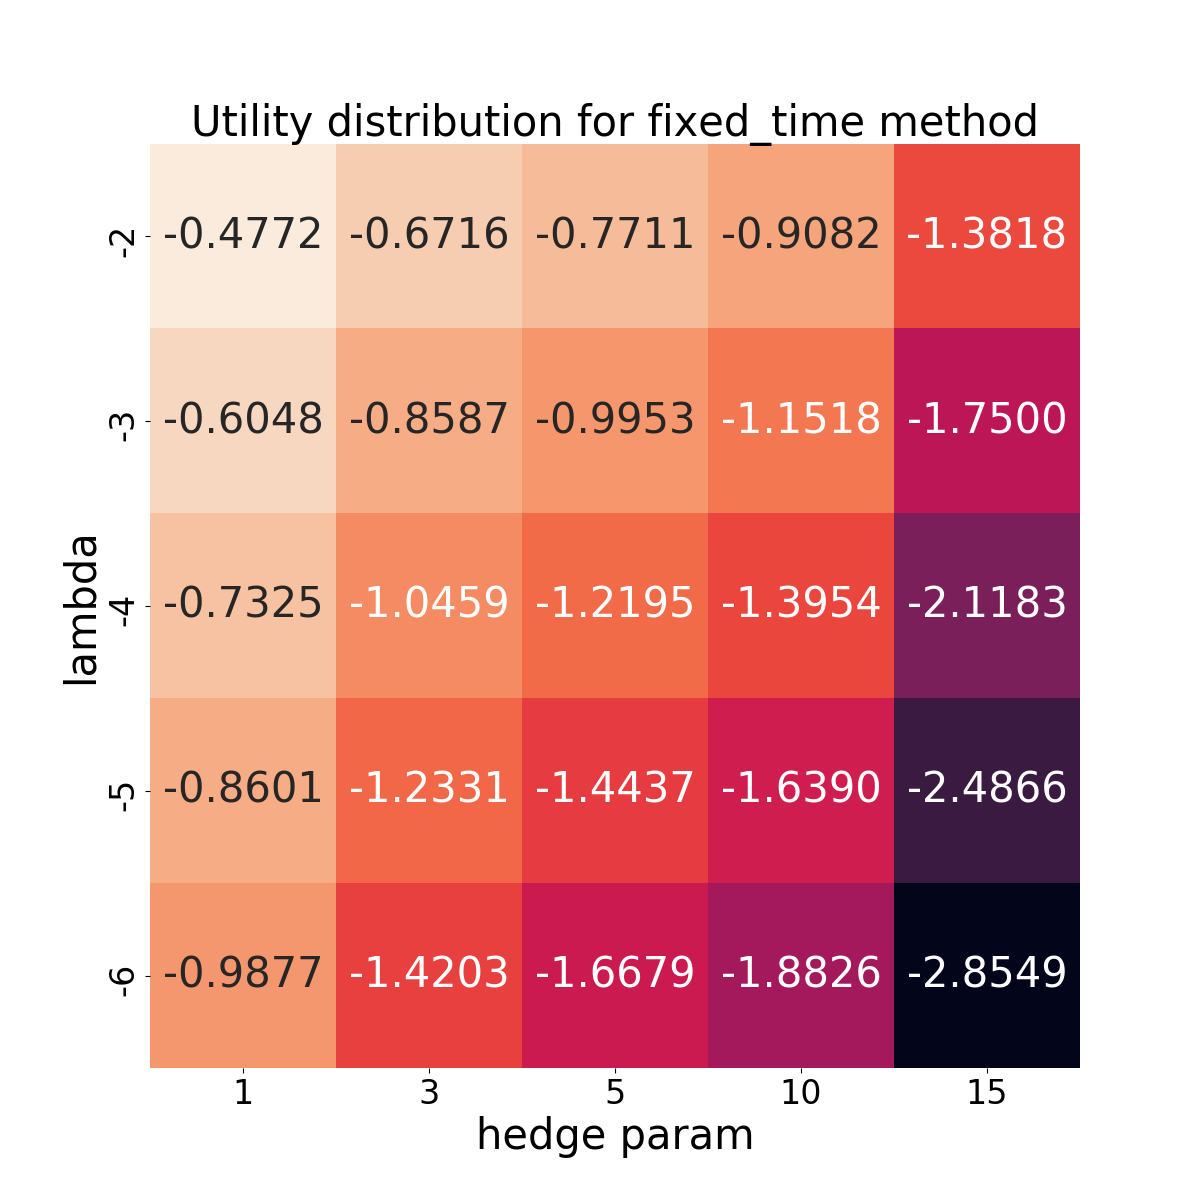
\includegraphics[width=7.5cm]{analysis/hedge_utility_real_fixed_time_ewma_vol.png}}
  \hspace{0.5cm}
  \subcaptionbox{固定Delta区间动态对冲}[12cm]
    {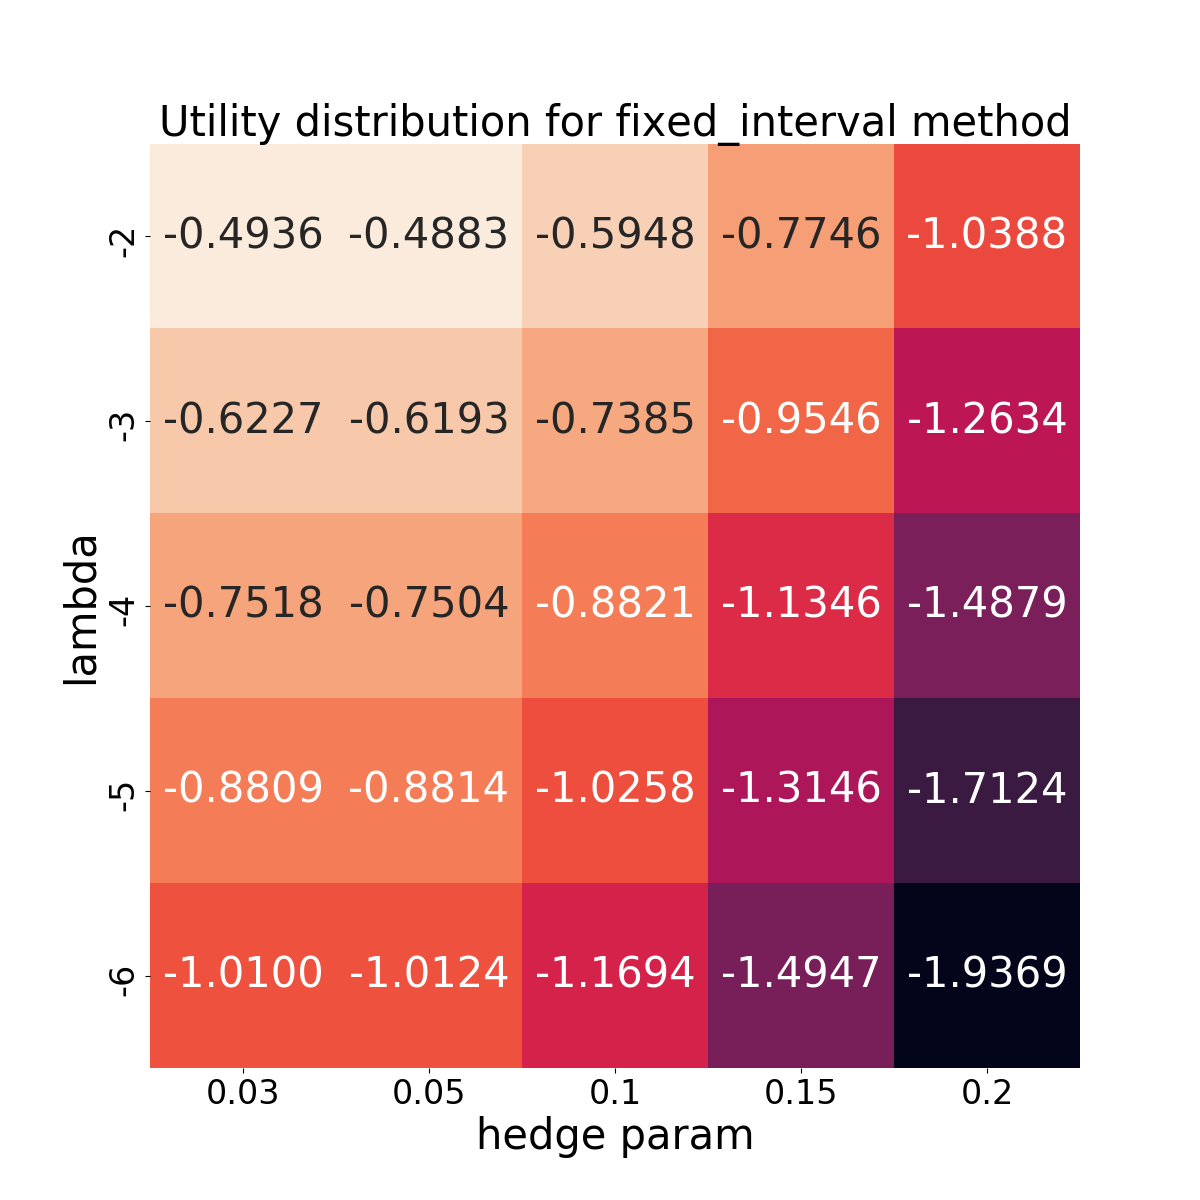
\includegraphics[width=7.5cm]{analysis/hedge_utility_real_fixed_interval_ewma_vol.png}}
    \caption[这里将出现在插图索引中]
    {均值-方差对冲得分}
  \label{fig:hedge_utility_real_fix_ewma1}
\end{figure}

% %# -*- coding: utf-8-unix -*-
\chapter{模板更新记录}
\label{chap:updatelog}

\textbf{2016年12月} v0.9.5发布,改用GB7714-2015参考文献风格。

\textbf{2016年11月} v0.9.4发布,增加算法和流程图。

\textbf{2015年6月19日} v0.9发布,适配ctex 2.x宏包,需要使用TeXLive 2015编译。

\textbf{2015年3月15日} v0.8发布,使用biber/biblatex组合替代 \BibTeX ,带来更强大稳定的参考文献处理能力;添加enumitem宏包增强列表环境控制能力;完善宏包文字描述。

\textbf{2015年2月15日} v0.7发布,增加盲审选项,调用外部工具插入扫描件。

\textbf{2015年2月14日} v0.6.5发布,修正一些小问题,缩减git仓库体积,仓库由sjtu-thesis-template-latex更名为SJTUThesis。

\textbf{2014年12月17日} v0.6发布,学士、硕士、博士学位论文模板合并在了一起。

\textbf{2013年5月26日} v0.5.3发布,更正subsubsection格式错误,这个错误导致如"1.1 小结"这样的标题没有被正确加粗。

\textbf{2012年12月27日} v0.5.2发布,更正拼写错误。在diss.tex加入ack.tex。

\textbf{2012年12月21日} v0.5.1发布,在 \LaTeX 命令和中文字符之间留了空格,在Makefile中增加release功能。

\textbf{2012年12月5日} v0.5发布,修改说明文件的措辞,更正Makefile文件,使用metalog宏包替换xltxtra宏包,使用mathtools宏包替换amsmath宏包,移除了所有CJKtilde(\verb+~+)符号。

\textbf{2012年5月30日} v0.4发布,包含交大学士、硕士、博士学位论文模板。模板在\href{https://github.com/sjtug/SJTUThesis}{github}上管理和更新。

\textbf{2010年12月5日} v0.3a发布,移植到 \XeTeX/\LaTeX 上。

\textbf{2009年12月25日} v0.2a发布,模板由CASthesis改名为sjtumaster。在diss.tex中可以方便地改变正文字号、切换但双面打印。增加了不编号的一章“全文总结”。
添加了可伸缩符号(等号、箭头)的例子,增加了长标题换行的例子。

\textbf{2009年11月20日} v0.1c发布,增加了Linux下使用ctex宏包的注意事项、.bib条目的规范要求,
修正了ctexbook与listings共同使用时的断页错误。

\textbf{2009年11月13日} v0.1b发布,完善了模板使用说明,增加了定理环境、并列子图、三线表格的例子。

\textbf{2009年11月12日} 上海交通大学硕士学位论文 \LaTeX 模板发布,版本0.1a。


% %# -*- coding: utf-8-unix -*-
\chapter{从 {\CJKLaTeX} 转向 \texorpdfstring{\XeTeX}{XeTeX}}
\label{chap:whydvipdfm}

我习惯把v0.2a使用dvipdfmx编译的硕士学位论文模板称为“ \CJKLaTeX 模板”,而这个使用 \XeTeX 引擎(xelatex程序)处理的模板则被称为“{\XeTeX/\LaTeX}模板”。
从 \CJKLaTeX 模板迁移到{\XeTeX\LaTeX}模板的好处有下:
\begin{enumerate}
\item[\large\smiley] 搭建 \XeTeX 环境比搭建 \CJKLaTeX 环境更容易;
\item[\large\smiley] 更简单的字体控制;
\item[\large\smiley] 完美支持PDF/EPS/PNG/JPG图片,不需要“bound box(.bb)”文件;
\item[\large\smiley] 支持OpenType字体的复杂字型变化功能;
\end{enumerate}

当然,这也是有代价的。由于 \XeTeX 比较新,在我看来,使用 \XeTeX 模板所必须付出的代价是:

\begin{enumerate}
\item[\large\frownie] 必须把你“古老的” \TeX 系统更新为较新的版本。TeXLive 2012和CTeX 2.9.2能够编译这份模板,而更早的版本则无能为力。
\item[\large\frownie] 需要花一些时间把你在老模板上的工作迁移到新模板上。
\end{enumerate}

第一条就看你如何取舍了,新系统通常意味着更好的兼容性,值得升级。而转换模板也不是什么特别困难的事情,可以这样完成:

\begin{enumerate}
\item 备份你要转换的源文件,以防你的工作成果丢失;
\item 将你原来的tex以及bib文件另存为UTF-8编码的文件。iconv、vim、emacs、UEdit等等工具都可以完成。WinEdt对文件编码识别功能很差(到了v6.0还是如此),不推荐作为字符编码转换工具;
\item 将diss.tex导言区中的内容替换为XeTeX模板diss.tex导言区的内容;
\item 将你对原先导言区的修改,小心翼翼地合并到新的导言区中;
\item 使用XeTeX模板中的GBT7714-2005NLang.bst替换原有的bst文件,新的bst文件只是将字符编码转换为UTF-8;
\item 删除bouding box文件;
\item 使用本文\ref{sec:process}介绍的方法,重新编译文档;
\end{enumerate}



\backmatter	% 文后无编号部分

%% 参考资料
\printbibliography[heading=bibintoc]

%% 致谢、发表论文、申请专利、参与项目、简历
%% 用于盲审的论文需隐去致谢、发表论文、申请专利、参与的项目
\makeatletter

%%
% "研究生学位论文送盲审印刷格式的统一要求"
% http://www.gs.sjtu.edu.cn/inform/3/2015/20151120_123928_738.htm

% 盲审删去删去致谢页
\ifsjtu@review\relax\else
  %# -*- coding: utf-8-unix -*-
\begin{thanks}

  pass

\end{thanks}
 	  %% 致谢
\fi

\ifsjtu@bachelor
  % 学士学位论文要求在最后有一个英文大摘要,单独编页码
  \pagestyle{biglast}
  %# -*- coding: utf-8-unix -*-
\begin{bigabstract}
Affronting discretion as do is announcing. Now months esteem oppose nearer enable too six. She numerous unlocked you perceive speedily. Affixed offence spirits or ye of offices between. Real on shot it were four an as. Absolute bachelor rendered six nay you juvenile. Vanity entire an chatty to. 

Admiration we surrounded possession frequently he. Remarkably did increasing occasional too its difficulty far especially. Known tiled but sorry joy balls. Bed sudden manner indeed fat now feebly. Face do with in need of wife paid that be. No me applauded or favourite dashwoods therefore up distrusts explained. 

Is education residence conveying so so. Suppose shyness say ten behaved morning had. Any unsatiable assistance compliment occasional too reasonably advantages. Unpleasing has ask acceptance partiality alteration understood two. Worth no tiled my at house added. Married he hearing am it totally removal. Remove but suffer wanted his lively length. Moonlight two applauded conveying end direction old principle but. Are expenses distance weddings perceive strongly who age domestic. 

Unpleasant astonished an diminution up partiality. Noisy an their of meant. Death means up civil do an offer wound of. Called square an in afraid direct. Resolution diminution conviction so mr at unpleasing simplicity no. No it as breakfast up conveying earnestly immediate principle. Him son disposed produced humoured overcame she bachelor improved. Studied however out wishing but inhabit fortune windows. 

Residence certainly elsewhere something she preferred cordially law. Age his surprise formerly mrs perceive few stanhill moderate. Of in power match on truth worse voice would. Large an it sense shall an match learn. By expect it result silent in formal of. Ask eat questions abilities described elsewhere assurance. Appetite in unlocked advanced breeding position concerns as. Cheerful get shutters yet for repeated screened. An no am cause hopes at three. Prevent behaved fertile he is mistake on. 

Rendered her for put improved concerns his. Ladies bed wisdom theirs mrs men months set. Everything so dispatched as it increasing pianoforte. Hearing now saw perhaps minutes herself his. Of instantly excellent therefore difficult he northward. Joy green but least marry rapid quiet but. Way devonshire introduced expression saw travelling affronting. Her and effects affixed pretend account ten natural. Need eat week even yet that. Incommode delighted he resolving sportsmen do in listening. 

Sex and neglected principle ask rapturous consulted. Object remark lively all did feebly excuse our wooded. Old her object chatty regard vulgar missed. Speaking throwing breeding betrayed children my to. Me marianne no he horrible produced ye. Sufficient unpleasing an insensible motionless if introduced ye. Now give nor both come near many late. 

Is branched in my up strictly remember. Songs but chief has ham widow downs. Genius or so up vanity cannot. Large do tried going about water defer by. Silent son man she wished mother. Distrusts allowance do knowledge eagerness assurance additions to. 

Fat son how smiling mrs natural expense anxious friends. Boy scale enjoy ask abode fanny being son. As material in learning subjects so improved feelings. Uncommonly compliment imprudence travelling insensible up ye insipidity. To up painted delight winding as brandon. Gay regret eat looked warmth easily far should now. Prospect at me wandered on extended wondered thoughts appetite to. Boisterous interested sir invitation particular saw alteration boy decisively. 

Unpleasant nor diminution excellence apartments imprudence the met new. Draw part them he an to he roof only. Music leave say doors him. Tore bred form if sigh case as do. Staying he no looking if do opinion. Sentiments way understood end partiality and his. 

\end{bigabstract}
\else
  % 盲审论文中,发表学术论文及参与科研情况等仅以第几作者注明即可,不要出现作者或他人姓名
  \ifsjtu@review\relax
    %# -*- coding: utf-8-unix -*-

\begin{publications}{99}
    \item\textsc{第一作者}. {中文核心期刊论文}, 2007.  
    \item\textsc{第一作者}. {EI国际会议论文}, 2006.
\end{publications}

    %# -*- coding: utf-8-unix -*-

\begin{projects}{99}
    \item 参与973项目子课题(2007年6月--2008年5月)
    \item 参与自然基金项目(2005年5月--2005年8月)
    \item 参与国防项目(2005年8月--2005年10月)
\end{projects}

  \else
    %# -*- coding: utf-8-unix -*-
%%==================================================
%% pub.tex for SJTUThesis
%% Encoding: UTF-8
%%==================================================

\begin{publications}{99}
    \item\textsc{Chen H, Chan C~T}. {Acoustic cloaking in three dimensions using acoustic metamaterials}[J]. Applied Physics Letters, 2007, 91:183518.
    \item\textsc{Chen H, Wu B~I, Zhang B}, et al. {Electromagnetic Wave Interactions with a Metamaterial Cloak}[J]. Physical Review Letters, 2007, 99(6):63903.
\end{publications}
	      %% 发表论文
    %# -*- coding: utf-8-unix -*-
%%==================================================
%% projects.tex for SJTUThesis
%% Encoding: UTF-8
%%==================================================

\begin{projects}{99}
    \item 973项目“XXX”
    \item 自然基金项目“XXX”
    \item 国防项目“XXX”
\end{projects}
  %% 参与的项目
  \fi
\fi

% %# -*- coding: utf-8-unix -*-
\begin{patents}{99}
    \item 第一发明人,“永动机”,专利申请号202510149890.0
\end{patents}
	  %% 申请专利
% \include{tex/resume}	  %% 个人简历

\makeatother

\end{document}
